
%\documentclass[DIV19]{scrartcl}
%\usepackage[paper size={90mm, 120mm},left=2mm,right=2mm,top=2mm,bottom=2mm,nohead]{geometry}
% FIXME try prettyref
\documentclass[oneside,a4paper,12pt,BCOR20mm,DIV14]{scrbook} % should be DIV14
%\documentclass{book}
% this gives a bit more than 2cm margin right and 4cm left
% koma-script.pdf: A4 is 210mmx297mm, BCOR is substraced before the page
% width is divided into DIV parts (HLU), a one sided leaves 1.5 HLU
% HLU*DIV=210-BCOR -> DIV=(210-BCOR)/HLU
% I want BCOR= 20mm 1.5 HLU = 20 mm 
% -> DIV=truncate(190*1.5/20) = truncate(14.25)=14
% I could use headinclude so that the header isn't printed into the margin

% Initially two softbound theses should be submitted to the
% Examinations Office for the examiners. Softbound theses should have
% the pages glued in.
% They don't need gold lettering on the spine.

%\includeonly{spatio-angular}

%\usepackage{enumitem}
%\setitemize{noitemsep,topsep=0pt,parsep=0pt,partopsep=0pt}

%\usepackage{etoolbox}

\pdfminorversion=5
% 9 is best zlib compression i use 0 while writing in the hope that
% git can track changes more easily
\pdfcompresslevel=0
% 3 is maximum for now
\pdfobjcompresslevel=0


\usepackage[utf8]{inputenc}
\usepackage[T1]{fontenc}
\usepackage[usenames,dvipsnames]{color}
\usepackage[onehalfspacing]{setspace} 
%\usepackage[draft]{graphicx}
\usepackage{graphicx}
\usepackage{longtable}
\usepackage{float}
\usepackage{wrapfig}
\usepackage{soul}
\usepackage{amssymb}
\usepackage{amsmath}

%\usepackage{pdfcomment}  % breaks hyperref metadata

% choose font here: http://www.tug.dk/FontCatalogue/mathfonts.html
\usepackage[T1]{fontenc}
%\usepackage[math]{iwona}
\usepackage[math]{kurier}
%\usepackage{cmbright}
\usepackage[scaled]{beramono}

\usepackage{footnote}

\usepackage{microtype}
\newcommand\Small{\fontsize{9}{9.2}\selectfont}
\newcommand*\LSTfont{\Small\ttfamily\SetTracking{encoding=*}{-60}\lsstyle}
\newcommand*\cmafont{\fontsize{8}{8.2}\selectfont\ttfamily\SetTracking{encoding=*}{-60}\lsstyle}






%\newcont\pdfcompresslevel


%\usepackage[hypertex,breaklinks]{hyperref} 
% breaklinks only seems to work with dvipdfm,
% otherwise urls have no
% line breaks

\usepackage[showrefs,showcites,ignoreunlbld]{refcheck} % for draft, uncomment for final

\usepackage[disable]{todonotes} % for draft, disable for final

\usepackage{lineno}
\usepackage[refpage]{nomencl}
%\special{background Black}\special{color Green}
%\usepackage[utf8x]{inputenc} 
%\usepackage[T2A]{fontenc} % for the russian reference
\usepackage{wasysym} %diameter
% http://www.andy-roberts.net/misc/latex/latextutorial3.html

%\usepackage{url} % natbib.pdf p.11 break urls up, seems to be done
                 % with hyperref, though

\usepackage{natbib}
%\usepackage{citeref}
\usepackage[pdftex,a4paper=true,plainpages,bookmarksnumbered,pagebackref,% put after natbib
pdftitle={Spatio-Angular Microscopy},%
pdfauthor={Martin Kielhorn},%
pdfkeywords={microscopy, photobleaching,%
  phototoxicity, spatial light modulator}, %
pdfsubject={PhD thesis}]{hyperref}


\usepackage{siunitx} %sudo apt-get install texlive-science
\usepackage{units}


% for app_hilo
\usepackage{listings}
\usepackage{color}
\usepackage{textcomp}
\usepackage{subfigure}


% \listfiles % show which files are loaded by tex

\bibpunct{(}{)}{;}{a}{}{,}
\makenomenclature
\newcommand{\vect}[1]{\mathbf{#1}}
\renewcommand{\r}{\vect r}
\renewcommand{\a}{\vect a}
\newcommand{\s}{\vect s}
\newcommand{\vnu}{\mbox{\boldmath{$\nu$}}}
\newcommand{\vmu}{\mbox{\boldmath{$\mu$}}}
\newcommand{\vtau}{\mbox{\boldmath{$\tau$}}}
\newcommand{\vrho}{\mbox{\boldmath{$\rho$}}}
\newcommand{\vvarrho}{\mbox{\boldmath{$\varrho$}}}
\newcommand{\supp}{\mathop{\mathrm{supp}}}
\newcommand{\pois}{\mathop{\mathrm{pois}}}
\newcommand{\step}{\mathop{\mathrm{step}}}
\newcommand{\diag}{\mathop{\mathrm{diag}}}
\def\k{\vect k}
\def\d{\vect d}
\def\e{\vect e}
\def\f{\vect f}
\def\c{\vect c}
\def\x{\vect x}
\def\y{\vect y}
\def\z{\vect z}
\def\q{\vect q}
\def\p{\vect p}
\def\l{\vect l}

\newcommand{\nvect}[1]{\vect{\hat{#1}}}
%\renewcommand{\i}{\nvect i}
\newcommand{\vi}{\nvect \i}
\def\hc{\nvect c}
\def\hs{\nvect s}
\def\hd{\nvect d}
\def\hx{\nvect x}
\def\hy{\nvect y}

\def\hz{\nvect z}
\def\n{\nvect n}
\def\t{\nvect t}
\def\m{\nvect m}
\def\vrho{\boldsymbol\rho}
\def\abs#1{\mathopen| #1 \mathclose|}


\renewcommand{\O}{\textsf{O}} % oxygen

% conclusions of paragraphs in the margin
%\usepackage[marginparwidth=2.5cm]{geometry}
\setlength{\marginparwidth}{2.2\marginparwidth}
\reversemarginpar
\newcommand{\cma}[1]{\marginpar{\cmafont{#1}}}
% include eps or pdf file, that was generated by inkscape, depending
% on if pdflatex or latex processes this file. latex allows a faster
% development cycle but pdflatex generates a smaller and better final
% pdf output
\def\svgending{\ifx\pdfoutput\undefined% 
  .eps_tex% 
  \else%
  .pdf_tex%
  \fi}

% use \svginput{1}{bla} to include bla.svg, make sure you keep this in
% one line, so that make can automatically find the dependencies with
% sed
\newcommand{\svginput}[2]{{\def\svgscale{#1}\input{#2\svgending}}}

\def\pdfending{\ifx\pdfoutput\undefined% 
  _vector.eps% 
  \else%
  _vector%
  \fi}
\newcommand{\pdfinput}[2]{\includegraphics[width=#1]{#2\pdfending}}

% example call \imagw{8cm}{bla.jpg}{bla}{caption abl}
\newcommand{\imagw}[4]{
  \begin{figure}[!hbt]
    \centering
    \includegraphics[width=#1]{#2}
    \caption{#4}
    \label{fig:#3}
  \end{figure}
}

\def\jpgending{\ifx\pdfoutput\undefined% 
  .eps% 
  \else%
  %
  \fi}
% use like this \jpginput{8cm}{imagefile}{caption ...  make sure all
% characters until the opening brace for the caption are on one line
\newcommand{\jpginput}[3]{\imagw{#1}{#2\jpgending}{#2}{#3}}

% this is for plots that are generated by gnuplot
\newcommand{\gnuplotinput}[2]{\begin{figure}[!hbt]%
    \centering%
    \includegraphics{#1_gnuplot}%
    \caption{#2}%
    \label{fig:#1}%
  \end{figure}}

\newcommand{\celegans}{\emph{C.~elegans}}
\DeclareMathOperator{\sign}{sign}
\DeclareMathOperator*{\sinc}{sinc}
\DeclareMathOperator*{\rect}{rect}

% reference to picture
\newcommand{\figref}[1]{\figurename~\ref{#1}}
\title{Spatio-angular microscope} % i don't call make title
\author{Martin Kielhorn}
% short summary at the beginning of a section
\newenvironment{summary}{\begin{quote}\small}{\end{quote}}

\begin{document}
\listoftodos
%\linenumbers
\begin{titlepage}
  
  \hspace{-4cm}
  \svginput{1}{objective-trace}



  \vspace{-5cm}
  
  \hspace{4cm}\textsf{\Huge Spatio--Angular Microscopy}
  
  \vspace{2cm}
  \hspace{6cm}\textsf{\huge PhD Thesis}


  \vspace{3cm}
  \hspace{4cm}\textsf{\Large Martin Kielhorn}
  
  \vspace{1cm}
  \hspace{4cm}\textsf{\Large April 2013}
\end{titlepage}
\newpage
%\include{abstract}
\section*{Abstract}
\begin{summary}
  Photobleaching and phototoxicity pose a problem in live cell
  imaging. Fluorescence imaging induces reactive oxygen species in
  observed organisms which can alter the behaviour of the
  sample. Hence, minimising the light exposure is an important goal.

  We augment a wide field epifluorescence microscope with two spatial
  light modulators. By controlling the spatial excitation pattern and
  the angle of illumination, we can adapt the illumination to the
  specimen. In many cases, this technique will create exposures with
  reduced excitation of the out-of-focus fluorophores, resulting in
  better image quality and less phototoxicity.

  Our custom software is used to obtain an initial image stack of the
  specimen. Subsequent image sections are exposed with excitation
  patterns that account for the previous image stack. Depending
  upon the distribution of fluorophores, this adaptive exposure can
  considerably reduce photobleaching and phototoxicity.
\end{summary}

\urlstyle{sf}
%\setcounter{tocdepth}{3}

\chapter*{Preface}
%\section*{Preface}

The work described in this thesis was carried out between June 2008
and April 2013.

In chapter \ref{sec:intro}, we introduce photophysics of fluorescence
and emphasize the importance of oxygen for phototoxicity. Furthermore,
we also explain conventional microscopes and CCD cameras.

In chapter \ref{sec:approaches}, we compare some state-of-the-art
techniques for illumination control in microscopes.  Particularly in
section \ref{sec:light-field-microscopy}, we discuss the micro-lens
based light field microscope by Levoy's computational photography
group, which imaged the toy soldier in 2003.

In chapter \ref{sec:setup}, we describe our microscope and in chapter
\ref{sec:experiments}, we show some images, taken with illumination
control in our prototype.

- ccd measurment

- mapping lcos camera

In the appendix, we also describe a completely different approach for
spatio--angular illumination based on holography (Appendix
\ref{sec:app_holo}) and we document an interferometric attempt to
convert our precise programmable phase mask into a spatial intensity
modulator (Appendix \ref{sec:app_dic}).

Note that the Appendix \ref{sec:dvi} describes a modification of our
prototype with a spatial light modulator that receives data from a
graphics card. A higher bandwidth makes this approach more useful than
the prototype described in the main text and we tried to implement
this first. However eventually, it proved too difficult to trigger the
components in this configuration and we switched to the more
predictable USB-controlled display as described in the main body of
the text.
 
The appendix also contains some theoretical explainations of
raytracing (Appendix \ref{sec:raytrace}), computational optical
sectioning (Appendix \ref{sec:app_hilo}) and the wave-optics based
simulation of our microscope (Appendix \ref{sec:sim-angle}).

\subsection*{Source Code Availability}

Source code that has been developed during this project is available
on \url{https://github.com/plops/mma}.  It contains implementations
for:
\begin{itemize}
\item illumination planning based on raytraces (see Appendix
  \ref{sec:raytrace})
\item moving the $z-$stage of a Zeiss Axiovert 200M microscope body
\item controlling an Andor Clara camera using the Andor SDK version
  2. For the other cameras following below, control software was written:
  \begin{itemize}
  \item Photometrics Cascade~II (interface to unsupported
    closed-source driver, only works on very old 32-bit Linux kernels)
  \item mvBlueFox 102G using the SDK
  \item Logitech Pro 9000 using a generic Video4Linux interface
  \item Andor sCMOS using Andor SDK version 3
  \end{itemize}
\item displaying patterns using a graphics card that supports OpenGL
  on a ForthDD SXGA ferroelectric LCoS display
\item controlling a stand-alone ForthDD WXGA 3DM display controller
  using USB
\item estimating the parameters of a rigid transformation between
  camera and LCoS display (see Appendix \ref{sec:rigid}),
\item controlling the micro-mirror array by Fraunhofer IPMS using
  their SDK
\item some specific image processing tools:
  \begin{itemize}
  \item three-dimensional convolution and Fourier transforms
  \item drawing of lines and ellipsoids in volumes
  \item rasterization of triangles (for creating shadow maps in the
    BFP, see section \ref{sec:trace-detect})
  \item calculation of optical transfer function for high NA
    objectives
  \item localization of spherical nuclei in volumetric data (parts of
    the algorithm as described in \citet{Santella2010})
  \end{itemize}
\end{itemize}
The main development was done using GNU~Linux. However, portability
was kept in mind and most of the code was made to work with Microsoft
Windows as well.

FIXME TRANSLATE:

Die Zeichnung auf der Titelseite zeigt den Strahlenverlauf durch ein
$100\times$ objective mit numerical aperture 1.45. Leider sind
Designparameter der von mir verwendeten Objektive kaum beizukommen
deshalb habe ich hier Daten aus einem Patent verwendet
\citep{Matthae2003}.


\subsection*{Acknowledgements}
It is my pleasure to thank all those who have made this thesis
possible. First and foremost, I owe my deepest gratitude to my
supervisor Rainer Heintzmann for giving me the opportunity to become
part of his research group at King's College London and later in the
Institute of Photonic Technology in Jena.

I owe my sincere thanks to Kai Wicker, Jakub Nedbal, Susan Cox, Daniel
Appelt, Ond\v rej Mandula, Ronny F\"orster, Ivana \v Sumanovac,
Eckhard Birkner, Kathrin Klehs and all the other members of our group
for valuable discussions, support and review of the manuscript.

My sincere thanks to the European Union Framework Programme 7 (project
number 2115597) for the studentship on this project.  I also thank
Erhard Ipp, G\"unter Z\"ochling, Vincent Galy, QueeLim Ch'ng, J\"org
Heber, Mark Eckert, Dirk Berndt, Joel Seligson, Jean-Yves Tinevez and
Florian R\"uckerl for helpful collaboration.

Furthermore I highly appreciate the input of Herbert Gross, Miroslav
Grajcar, Edward Rosten, Christophe Rhodes, Paul Khuong, Nikodemus
Siivola, Gabor Melis and Lu\' is Oliveira. Occasionally, the expertise
and insight of them steered me into right direction or greatly
simplified problems I faced.

Finally, I wish to thank the authors and contributors to the following
software projects: Linux, GCC, Emacs, SBCL \citep{Rhodes2008}, Maxima
\citep{Maxima.sourceforge.net2013}, Micromanager
\citep{Edelstein2010}, DIPimage \citep{dipimage}, Wireshark
\citep{wireshark}, Latex, Inkscape \citep{inkscape}, Gimp
\citep{gimp}, ImageJ/Fiji \citep{Abramoff,Schindelin2012} and Blender
\cite{blender}.  These free software projects and their communities
are invaluable to my work and greatly enhance my efficiency.

The work presented in this thesis is my own, unless I cite a
reference.

\begin{flushright}
  M.~K.
\end{flushright}

\noindent
Jena, Germany

\noindent
April 2013



\newpage
\tableofcontents
\printnomenclature



\chapter{Introduction}
\label{sec:intro}
\begin{summary}
  In this work I discuss a modification of a fluorescence microscope    \cma{my device}
  that minimizes the toxic effects of the excitation light.

  In the following introductory chapter I describe what phototoxicity   \cma{phototoxicity}
  is and how it comes about. Then I give an example of how it
  influences biological observations in a developing \celegans\ 
  embryo and describe how this particular biological system can be
  used to evaluate and compare the phototoxicity of different microscopes.

  Later in this chapter I give an overview of image formation   \cma{cameras}
  in the wide-field microscope and I describe its principle limitations
  regarding resolution and depth discrimination. Furthermore, I
  discuss the two most important current image detector technologies
  --- electron multiplying charge-coupled devices (EMCCD) and
  scientifc complementary metal–oxide–semiconductor (sCMOS).
\end{summary}
\nomenclature{EM-CCD}{Electron multiplying charge-coupled devices}
Regardless of whether it is the picture of earth captured by an
orbiting satellite, the x-ray motion picture of a running dog or the
time-lapse recording of a blooming flower. Images capture our
imagination and they are a good starting point to develop new models
and theories.

This is particularly true for microscopy.  Only after people became
aware of microorganisms by direct observation, medieval quack could
finally be overcome and modern medicine based on the scientific
method flourished instead.

Even today --- with electron microscopes, magnetic resonance
tomography and sequencing machines --- optical microscopy still is an
indispensable tool for research of living organisms.

Fluorescence microscopy is of particular importance: It enables the     \cma{labelling, switching}
scientist to selectively label a particular type of molecule in living cells
and observe how they perform their biological function.

Besides localizing molecules it is possible to measure physical
quantities inside of the sample. There are, for example, fluorescent
labels that report membrane potentials or viscosity inside of cells.

Finally, it is even possible to exert a controlling function with the
excitation light: There are compounds that locally release chemicals
when illuminated and there are  genetically encoded ion channels that can be
switched by light \citep{Boyden2005}.

However, the excitation light introduces unnatural and potentially
deleterious energy into the specimen. If the exogenous light harms the
observed organism in any way, this effect is called phototoxicity.

% dennoch: from photophysical prospective of single- and multi-photon
% microcopy, probably the most disheartening reality is the occurrence
% of photobleaching and photodamage
% \citep{diaspro2009nanoscopy}

There are a number of techniques that can reduce phototoxicity: Two
photon excitation, controlled light exposure, selective plane
illumination, highly inclined and laminated optical sheet, and oblique
plane microscopy. I introduce them in
chapter \ref{sec:approaches}. These techniques have different
pros and cons and not all are equally suited for a specific problem,
e.g.\ selective plane illumination is very effective, but it needs two
perpendicular lenses and can not be used for multiwell plates or to
observe the liver of a living, adult mouse.

In this work I present an approach that makes use of modern display
and camera technology. We only modify the microscope's illumination
path, the space around objective lens and specimen remains as
accessible as in any conventional wide-field microscope.



\section{Phototoxicity in life sciences and the model organism
  \celegans}
\label{sec:intro-phototoxicity}
The partner in our project who is responsible for decisions related to
life sciences and biology is Institut Pasteur (Paris, FR). They work
on infectious diseases. 

In order to motivate the importance of phototoxicity, I would like to
portray an elegant drug screening experiment which I have seen on one
of my visits in Paris: An automatic microscope continuously images a
cell culture in multiwell plates. These cells carry a pathogen. The
pathogen, the nuclei of the cultured cells and the membranes of the
cells are each stained with a different fluorophore. The cells in each
well of the plates are exposed to a different chemical.

A chemical is considered a hit and will be investigated during further
trials, when the time lapse images show that the culture cells stay
healthy and the number of pathogens decrease. As neither people nor
animals come to harm, this screening experiment is an impeccable
method to systematically understand and hopefully heal certain
diseases. However, this experiment does not work very well, if the
excitation light --- and not the drug --- kills the pathogens. The
effect of phototoxicity should therefore be minimized.


Now one would hardly develop a microscope and directly test it with
dangerous pathogens. As part of our collaboration, the Institut
Pasteur therefore developed a safe biological test system that is
relatively easy to maintain \citep{Stiernagle2006} and allows to test
the phototoxicity of various microscopes \citep{Tinevez2012}.




The basis of the system is the embryo of the organism \celegans. These
are small invertebrates. The adult form is approximately \unit[1]{mm}
long.  Their anatomy and development are comparatively simple and have
been well characterized \citep{Sulston1977,Durbin1987}.

\begin{figure}[hbtp]
  \centering
  \svginput{1}{celegans-devel-sb}
  \caption{Phototoxic effects while imaging the embryonal development
    of three \celegans\ embryos (strain AZ212, histone-2B tagged with
    eGFP) with different excitation intensities. The embryo with
    lowest excitation dosage (left) develops fastest. The embryo with
    the highest dosage (right) ceases development and nearly all
    fluorophores are bleached after the experiment. Images by
    J.-Y. Tinevez using a Zeiss LSM700 confocal microscope (Institut
    Pasteur, Paris, FR).}
  \label{fig:celegans-devel}
\end{figure}


% \jpginput{12cm}{celegans-devel}{Phototoxic effects while imaging the
%   embryonal development of three \celegans\ embryos (strain AZ212,
%   histone-2B tagged with eGFP) with different excitation
%   intensities. The embryo with lowest excitation dosage (left)
%   develops fastest. The embryo with the highest dosage (right) ceases
%   development and nearly all fluorophores are bleached after the
%   experiment. Images by J.-Y. Tinevez using a Zeiss LSM700 confocal
%   microscope (Institut Pasteur, Paris, FR).}
  

We use embryos of a genetically modified strain\footnote{Our strain
  has WormBase ID AZ212 \citep{Praitis2001}.} that expresses eGFP
tagged histones (enhanced green fluorescent protein, excitation
maximum \unit[488]{nm}, emission maximum \unit[509]{nm}). Histones are
incorporated into the chromatin during cell divisions, i.e.\ the
nuclei of our worms fluoresce green.  The mother worm passes a
sufficient amount of these proteins into the cytoplasm of the
embryo. In the beginning of its development the embryo entirely relies
on this reserve of histones. Only in a much later stage --- certainly
not during the first few hours, that we observe --- it will form its
own histones.

\figref{fig:celegans-devel} compares time-lapse experiments on three \cma{embryo example} 
different \celegans\ embryos with varying
excitation intensities.

The lineage tree of two developing \celegans\ embryos is the \cma{reproducible development}
same.  With all other factors being equal, particularly if the
temperature is constant at $\unit[21\pm
1]{\degreeCelsius}$, two different embryos will develop at the
same speed from egg to fertile adult in three and a half days.


At the beginning of the experiment, embryos are removed from their
mothers at an identical stage, before any cellular divisions have
occured. Then a $z-$stack of the egg with 41 slices and one micron
$z-$sampling is obtained every two minutes.

The columns in \figref{fig:celegans-devel} depict three different embryos
whose development was imaged according to this protocol for two hours
and 38 minutes with different excitation powers.

The figure displays the maximum intensity projections of the
$z-$stacks.  In order to make the cell nuclei visible in all images, I
normalized the data to the same range. As can be guessed from the
photon shot noise, the upper left image contains the least number of
fluorescence photons, and the upper right the most.

An analysis of the time-lapse data show that one hour into the
experiment the embryo with the highest excitation dose (right) has
stopped developing and its fluorophores are strongly bleached.  Some
cells even turned apoptotic and went into programmed cell death.

After two hours and 38 minutes the experiment was stopped and the
embryo which was exposed to the lowest dose (left) has developed the
largest number of cells. The middle embryo ceased developing while the
right embryo died even earlier and nearly all its fluorophores are
bleached at the end of the experiment.

In \figref{fig:worm-integration-time} I reproduce quantitative data
from \cite{Tinevez2012}. Each data point in this graph corresponds to
a two hour time-lapse imaging experiment of a \celegans\ embryo in a
wide-field microscope. From a very low excitation up to a certain
threshold dose the development is not affected by the light and
approximately 50 cells develop during the two hours.

For a dose above the threshold the development is slowed due to
phototoxicity and the number of cells at the end of the experiment
decreases.

\gnuplotinput{worm-integration-time}{Longer exposure times are less
  phototoxic. Each data point corresponds to one embryo that developed
  under a particular excitation dose for two hours. The solid lines
  are sigmoidal fits to the data. Also indicated are the two
  phototoxicity thresholds given by the inflection point of the
  sigmoid and their $95\%$ confidence intervals. This data was
  provided by J.-Y. Tinevez (Institut Pasteur, Paris, FR) and is also
  published in \cite{Tinevez2012}.}  

The orange data points in the diagram correspond to a per slice
integration time $\tau$ of \unit[100]{ms} and for the green data
the integration time is five times higher.

\nomenclature{$\Omega$}{Excitation dose in $\joule/(\centi\meter^2\textrm{stack})$} 
\nomenclature{$\Phi_e$}{Radiant flux of excitation light in watts} 
The dose $\Omega$ on the $x-$axis is calculated as
\begin{align}
\Omega = \frac{\Phi_e n \tau}{A},
\end{align}
with integration time $\tau$, area $A$ of the illuminated field, the
number of slices $n=41$ and radiant flux $\Phi_e$ of the excitation
light, as measured in the pupil.

Naively one would assume that it should not make any difference if the
excitation light dose is administered with \unit[100]{ms} or
\unit[500]{ms} exposures but these data show that a longer exposure
time and low intensity are less phototoxic.

These results agree with an earlier study in tobacco plants
\citep{Dixit2003}. They investigate cell death a few days after
illumination and find that there is a threshold dose below which no
phototoxicity can be detected, and that this threshold decreases with
light intensity. Dixit and Cyr show that the damage is caused by
reactive oxygen species and they explain the shift of the
phototoxicity threshold by the limited capacity of the cells'
scavenging system for those radicals. They also predict the existence
of redox-sensitive checkpoints in the mitotic division cycle.

%\citep{Sancar2004}

In summary this section describes how to measure phototoxicity with
biological specimen.  The next section gives an overview of the
underlying photophysics and the rest of this work describes our
attempt to build a microscope with reduced phototoxic footprint.



\section{Photophysical principles of phototoxicity}
\label{sec:photophysics}
\begin{summary}
  Here I give a short overview of fluorescence of molecules in order
  to introduce the terms photobleaching and phototoxicity.
\end{summary}
A fluorophore is a molecule that can absorb and subsequently emit
light. During the absorption of a photon the molecular orbital
transitions from the electronic ground state $S_0$ to an excited state
$S_1$. The lifetime of the excited state $S_1$ is in the order of a
few nanoseconds.
\begin{figure}[!hbt]
  \centering
  \svginput{.8}{flu-level}
  \caption{The Jablonski energy level diagram of an illustrative
    fluorescent molecule. The boxes depict orbitals, up and down
    arrows symbolize the spin of the outer electrons. Fat horizontal
    lines represent electronic states. Thinner lines indicate
    vibro-rotational states. Various processes are shown with their
    typical time scales. VR = vibro-rotational relaxation, ISC =
    intersystem crossing, IC = internal conversion \cite[inspired
    from][]{Haken2006}.}
  \label{fig:flu-level}
\end{figure}
A Jablonski diagram, as depicted in \figref{fig:flu-level}, summarizes
information \cma{energy levels} about the energy levels of a molecule
and possible transition processes.

%  If the photon has an even higher
% energy, the electron will go into the second excited singlet state
% $S_2$.

The majority of known stable and bright fluorophores absorb and emit
in the wavelength range between \unit[300]{nm} and \unit[700]{nm}.
Photons at the high energy end of this range can excite molecules into
higher energy levels $S_n, (n>1)$ than the first excited state; these
states are unstable and hardly return to the ground state $S_0$. On
the other side of the spectrum: a molecule that absorbs in the
near-infrared ($\unit[>700]{nm}$) has a low-lying excited singlet
state $S_1$ and therefore potentially increased reactivity and a high
probability for a non-radiative transfer back into the ground state
$S_0$ \citep{Sauer2011}.


The term \emph{Stokes' shift} describes the frequency shift between
the absorbed and emitted photon; the energy difference is lost as heat
to the fluorophore molecule and surrounding solvent.  For the
practical implementation of fluorescence microscopes this is
significant, as it enables to separate excitation and emission light
with a dichromatic beam splitter.


The excitation probability of a fluorescence molecule depends on the
orientation of its dipole axis relative to the plane of vibration of
the excitation field. Especially if the molecule is not rigidly bound
to a bigger structure or embedded in a viscous solvent it will
reorient its dipole during the fluorescence lifetime and emit the
fluorescence photon in a random direction. We use this in the next
section to describe image formation in the fluorescence microscope.


The triplet states $T_n$ play an important role in photobleaching.
Pure electronic absorption of one photon has no effect on the spin of
an electron and therefore the transition from singlet states $S_n$
into the triplet state $T_n$ should not occur. However, interaction
with the nuclei can mediate this spin transition. Therefore, in
fluorophores this transition has a small probability, resulting in
long lifetimes of the triplet state $T_1$.

\cite{Deschenes2002} show that excitation of higher triplet states
$T_n$ is the predominant reactive process for photobleaching in
vacuum. In particular they measured that one rhodamine~6G molecule
\emph{in vacuum} can emit more than \num{1e9} photons before it
bleaches, if the excitation intensity is low enough
$(\sim\unit[1]{\si{\watt/\cm^2}})$ to prevent decay over triplet
states.

In normal atmosphere the prolonged lifetime of the triplet state $T_1$
makes it highly likely for the fluorophore to react with molecular
oxygen $\O_2$. Oxygen is abundant and has a triplet ground state
${}^3\Sigma$ with two unpaired electrons of parallel spin in its
$\pi^*-$orbitals (see \figref{fig:oxygen}).

  \citep{Bernas2004}

\begin{figure}[!hbt]
  \centering
  \svginput{1}{oxygen}
  \caption{{\bf left:} Schematic that depicts how the orbitals of the
    oxygen molecule are formed from the atomic orbitals. {\bf right:}
    Molecular oxygen has the lowest energy in its triplet state
    ${}^3\Sigma$ where the spins of the two outer $\pi^*-$electrons
    are parallel. Inspired from \citet{Linde2011a}.}
  \label{fig:oxygen}
\end{figure}

If a ground-state oxygen molecule comes into physical contact with a
$T_1$ fluorophore, the energy of the latter can be transferred by an
electron exchange energy transfer mechanism in which the orbitals
directly interact with each other \citetext{\citealp[p.~438]{Haken2006} and
  \citealp{Linde2011a}}.

During this reaction, which is also known as triplet--triplet
annihilation, two forms of singlet oxygen form in competition: The
lower energy state ${}^1\Delta$ and the short-lived, higher energy
state ${}^1\Sigma$ that immediately ($T_{1/2}\sim\unit[10^{-9}]{s}$)
sends out a \unit[1268]{nm} photon and decays into ${}^1\Delta$.

The resulting singlet oxygen ${}^1\Delta$ is very reactive. In a
typical specimen it diffuses only a few tens of nanometres until it
reacts with another molecule.

%(FIXME 2000 greenbaum measures oxygen production, bernas 2004 anoxia gfp)

Nowadays many methods are known to reduce photobleaching: Substitute
oxygen with noble gases or remove it enzymatically
\citep[p.~89]{Sauer2011}, depopulate the triplet state by adding
reducing as well as oxidizing agents to the solvent
\citep{Vogelsang2008} or couple a triplet quencher directly to the
fluorophore \citep[p.~19]{Sauer2011}. For fixed samples it helps to
change the solvent or polymer.
 
In living specimen these techniques may reduce photobleaching, but
they can also have a detrimental effect on the biological system
itself. Removing oxygen will quite certainly have a negative
effect. In order to reduce phototoxicity it makes sense to think about
the light management in the microscope.


\section{Conventional microscopes}
\begin{summary}
  The wide-field fluorescence microscope does not excite fluorophores
  of the specimen in an optimal way. In this section I outline how
  these microscopes work and explain how out-of-focus blur severely
  limits their performance. I introduce the terms point spread
  function, optical transfer function and etendue.
\end{summary}

\subsection{Ray-optical description of a large-aperture lens}

A microscope, is a device that collects light coming from one plane  \cma{lateral image}
and forms a magnified image on a
camera. \figref{fig:widefield-microscope}~b) shows a schematic
representation of the detection path of a wide-field microscope.

The main components are an objective lens with focal length $f$ and a
\cma{telecentricity} tube lens TL1 with focal length
$f_\textrm{TL}>f$. Sample, lenses and camera are arranged in
double-telecentric configuration, i.e.\ the sample is located in the
front focal plane of the objective, the tube lens is at distance
$f_\textrm{TL}$ behind the pupil (i.e.\ the back focal plane of the
objective) and the camera is in the focal plane behind the tube lens.
\nomenclature{TL}{Tube lens}

%FIXME our microscope is only telecentric with respect to the object side

\nomenclature{$\beta$}{Transversal magnification of an objective
  $\beta=f_\mathrm{TL}/f$, for Zeiss lenses the magnification $\beta$
  is written on the objective and the focal length of the tube lens is
  defined as $f_\textrm{TL}=\unit[164.5]{mm}$}


Light from the sample is collimated by the objective lens and
\cma{lateral magnification} re-imaged by the tube lens. The lateral
magnification $\beta$ is given by the ratio of the focal lengths of
the two lenses:
\begin{align}
  \beta=\frac{\overline{O'P'}}{\overline{OP}}=\frac{f_\mathrm{TL}}{f}. \label{eq:beta}
\end{align}
Note that in \figref{fig:widefield-microscope}~b) I represent the
objective lens as a single element.  This is a simplification.

In the paraxial limit ray-tracing calculations for a thick lens or
even several consecutive lens elements can be simplified by bending
the ray only at one place --- at the principal plane.

\nomenclature{marginal ray}{Axial ray through the periphery of the
  entrance aperture}

\nomenclature{chief ray}{Ray from the periphery of the field through
  the center of the entrance aperture}

\nomenclature{entrance aperture}{Projection of the limiting aperture
  of the optical system into object space}


Microscope objectives must collect light from a large aperture in
\cma{perfect imaging and high-aperture} order to produce a high
resolution image. This is a fact I will support shortly using the
wave-optical model. Unfortunately, the large ray angles in the
objective prevent its simplified description using principal planes,
but an analysis using the eikonal theory \citep{Haferkorn1984} shows % page 125 2.3.2 mikroobjektive65g ggggg g gg g v g      v  v--*


that an optical system that fulfills the Abbe sine condition allows
perfect imaging even for widespread ray bundles.
\begin{align}
  \label{eq:sine-condition}
  \beta = \frac{n \sin\alpha}{n' \sin\alpha'} \qquad \textrm{(Abbe sine condition)}
\end{align}
This condition ensures that the focal length, a quantity which is
usually defined only for paraxial rays, is equal for all angles.  This
in turn means that such a lens carries out a Fourier transform from
the front to the back focal plane with linear scaling. Note that a
lens with a non-linear distortion in the back focal plane, such as given by the concept of a thin lense used at large angles, will fail to
produce an image that is similar to the object.

It turns out that ray bending\label{aplanatic} in a high-aperture lens
system that \cma{aplanatic sphere} fulfills the Abbe sine condition
can be simplified to a one bend at a single surface, quite similar to
the utilization of principal planes in paraxial optics. For a
high-aperture system this surface is no longer a plane.  Instead it is
a sphere with radius $n f$ and called \emph{aplanatic sphere}.  The
refractive index $n$ accounts for an immersion medium on the object
side.  I depict the aplanatic surface as two circle segments with a
bold red curve on each of the lenses in
\figref{fig:widefield-microscope}~b).

In addition to the Abbe sine condition, microscope lenses are also
corrected for spherical aberration and linear coma \citep{Gross2005}.
Then the coma rays are symmetric around the chief ray, the wavefront
and point spread function are approximately invariant for small field
sizes (in first order).  This ensures that the imaging conditions are
invariant for small regions of the field plane and allows to express
image formation with linear systems theory.

\figref{fig:widefield-microscope}~c) shows the illumination of a
widefield fluorescence microscope with a laser. A dichromatic beam
splitter (BS) separates illumination and returning fluorescence light.

\subsection{Wave-optical theory for image formation in a fluorescence microscope}
In the following sectoin I will describe how the image on the camera
\cma{wave optics} is formed. For this one has to use wave theory
because close to the image rays intersect, invalidating ray-optical
predictions. As both wave-optical and ray-optical theory, are very
much related, one can give a useful interpretation of the aplanatic
surface for wave optics.

The underlying Maxwell equations and the wave equation are linear and   \cma{plane waves}
we can represent propagating solutions (evanescent solutions are
neglected) of the wave equation as a superposition of the elementary
solution --- the monochromatic, plane waves described by wave vector
$\k$:
\begin{align}
  u(\r,t)=u\,\exp(i(\k\r-\omega t)),\quad \r=(r_x,r_y,r_z),\
  \k=(k_x,k_y,k_z),\ |\k|=2\pi \underbrace{n/\lambda_0}_{1/\lambda},
\end{align}
with vacuum wavelength $\lambda_0$, refractive index $n$ and
wavelength $\lambda$ in the immersion medium.

The accurate treatment of high-aperture optics would in fact require a
vectorial calculation of the image for a fluorophore with a particular
dipole orientation.  Subsequently these images should be averaged to
account for random fluorophore orientations, but as I do not need
quantitative expressions, I limit myself to the simpler scalar problem
which provides qualitatively similar results.
% \begin{figure}[!hbt]
%   \centering
%   \svginput{1}{sine-condition}
%   \caption{dasfklj}
%   \label{fig:sine-condition}
% \end{figure}

\begin{figure}[!hbt]
  \centering
  \svginput{1}{widefield-microscope}
  \caption{{\bf a)} Segment of the three-dimensional frequency
    spectrum of the light from the sample that is collected by the
    objective lens is highlighted in red on the Ewald sphere. {\bf b)}
    Schematic of the detection path of a modern microscope. The sample
    is in the front focal plane of the objective. The detection tube
    lens TL1 forms a magnified image on the camera. The image points
    are denoted by $O'$ and $P'$. The aplanatic spheres for objective
    and tube lens are indicated in \textcolor{red}{red}. {\bf c)}
    Parallel laser epifluorescence excitation. The excitation tube
    lens TL2 focuses a laser into the pupil of the objective. The beam
    is reflected by a dichromatic beam splitter (BS) towards the
    objective. An extended area in the specimen is
    illuminated. Fluorescence light returns through the objective, is
    transmitted through BS and forms an image on the camera. }
  \label{fig:widefield-microscope}
\end{figure}
Assuming that the excited fluorophores in the sample give rise to a
\cma{Ewald sphere} monochromatic electromagnetic field --- I simplify
the problem by omitting the complication that fluorophores emit
photons in a wavelength range --- then using the spatial frequency
vector $\vnu=\k/(2\pi)$ we can expand the three-dimensional,
stationary field amplitude distribution $u(\r)$ into its spatial
frequency spectrum $\widetilde u(\vnu)$:

\nomenclature{$u(\r)$}{Scalar field as a function of spatial
  coordinates} 

\nomenclature{$\widetilde u(\vnu)$}{Fourier transform
  of scalar field as a function of spatial frequencies}

\nomenclature{$\r=(r_x,r_y,r_z)^T$}{Three-dimensional spatial
  coordinate} 

\nomenclature{$\r_t=(r_x,r_y)^T$}{Transversal two-dimensional spatial
  coordinate}

\nomenclature{$\vnu=(\nu_x,\nu_y,\nu_z)^T$}{Three-dimensional spatial
  frequency}

\nomenclature{$\vnu_t=(\nu_x,\nu_y)^T$}{Transversal two-dimensional
  spatial frequency}


\begin{table}[!hbt]
  \centering
  \begin{tabular}{ l l | l }
    $u(\r):$&$ \mathbb{R}^3\to\mathbb{C}$ & field distribution in sample space \\
    $u'(\r'):$&$\mathbb{R}^3\to\mathbb{C}$ & field distribution in image space \\
    $S(\r):$ & $\mathbb{R}^3\to\mathbb{R}$ & distribution of fluorophores in sample space \\
    $I'(\r'):$&$\mathbb{R}^3\to\mathbb{R}$ & intensity distribution in image space\\
    $\widetilde u(\vnu):$&$\mathbb{R}^3\to\mathbb{C}$ & spatial frequency spectrum of field in sample space \\
    $a(\r):$&$\mathbb{R}^3\to\mathbb{C}$ & amplitude point spread function \\
    $\widetilde a(\vnu):$&$\mathbb{R}^3\to\mathbb{C}$ & amplitude transfer function, generalized aperture \\
    $h(\r)=|a(\r)|^2:$&$\mathbb{R}^3\to\mathbb{R}$ & intensity point spread function \\
    $\widetilde h(\vnu):$&$\mathbb{R}^3\to\mathbb{C}$ & optical transfer function \\
  \end{tabular}
  \caption{Overview of the functions that are used in this section.}
  \label{tab:widefield-functions}
\end{table}



\begin{align}
  u(\r)=\mathcal{F}(\widetilde u(\vnu)):=\int_{-\infty}^{\infty}\int_{-\infty}^{\infty}\int_{-\infty}^{\infty}
  \widetilde u(\vnu) \exp(2\pi i \r\vnu)\ \textrm{d}^3 \vnu
\end{align}
Where $\mathcal{F}$ denotes the Fourier transform operation. I will
use several functions in this section. See
Table~\ref{tab:widefield-functions} for a listing of their names.

Since we have assumed a monochromatic field and the length $|\vnu|$ of
the spatial frequency vector is the inverse of the wavelength
($n/\lambda_0$), in the material of refractive index $n$, the support
(denoted '$\supp$') of this spectrum $\widetilde u(\vnu)$ is limited
to the surface of a sphere of radius $n/\lambda_0$:
\begin{align}
  \supp \widetilde u(\vnu) &= \{\vnu \in \mathbb{R}^3: |\vnu|=n/\lambda_0\}.
\end{align}
This sphere is the transfer function of free space, and is also called
Ewald sphere (see \figref{fig:widefield-microscope}~a)).  \nomenclature{Ewald sphere}{Transfer function of free
  space} Scaling the Ewald sphere with $f\lambda_0$ gives the
aplanatic surface of the lens. Note that the $x-$component of the
marginal ray (in the $xz-$plane) corresponds to the spatial frequency
component $\nu_x = n\sin\alpha$ in object space and
$\nu_x'=n'\sin\alpha'$ with $n'=1$ in image space. The transversal
spatial frequency components are related due to the Abbe sine
condition (\ref{eq:sine-condition}):
\begin{align}
  \beta &= \nu_x/\nu_x',\quad  \beta = \nu_y/\nu_y'.
\end{align}
The transfer function $\widetilde a(\vnu)$ of the lens is defined by
complex values on the Ewald sphere \citep{McCutchen1964}:
\begin{align}
  \widetilde a(\vnu)&=\exp\left(2\pi i \frac{ n}{\lambda_0} 
    W(\vnu_t)\right)
  \delta\left(\frac{n}{\lambda_0}-|\vnu|\right)  \step\left(|\vnu|cos(\alpha)-\nu_z\right), \label{eq:mccutchen} \\
  \step(x)&=
  \begin{cases} 
    1 & x\ge 0 \\
    0 & x<0 
  \end{cases}, \qquad \textrm{(Heaviside step function)} \label{eq:unit-step}
\end{align}
with the Dirac delta function $\delta$, transversal spatial frequency
vector $\vnu_t=(\nu_x,\nu_y)^T$ and the wavefront error
$W(\vnu_t)$. McCutchen calls the three-dimensional function
$\widetilde a(\vnu)$ the generalized aperture.

For this discussion I set $W(\vnu_t)=0$, i.e.\ there is no wavefront
aberration and the lens is diffraction limited. Furthermore, The
Heaviside step function limits the size of the calotte (or cap) of the
Ewald sphere that is defined by the acceptance angle $\alpha$ of the
objective.

Just as the objective lens, the tube lens can be described by its
generalized aperture but I assume that the tube lens maintains a
diffraction limited wavefront of the full angular range. For this
discussion, the full microscope is readily described by the
generalized aperture of just its objective lens.

Multiplication of the emission angular frequency spectrum $\widetilde u(\vnu)$
with the generalized aperture $\widetilde a(\vnu)$ gives the angular
frequency spectrum of the amplitude in the image plane:
\begin{align}
  \widetilde u'(\vnu') = \widetilde u'(\vnu/\beta) = \widetilde u(\vnu/\beta)\cdot \widetilde a(\vnu/\beta).
\end{align}
Note that I use the transversal magnification $\beta$ to scale the
arguments of the functions, so that the result is given in image space
spatial frequencies\footnote{Unfortunately, my notation is slightly
  problematic here. I assume that $z-$sampling occurs by stepping the
  sample through the object space while the camera is fixed in the
  focal plane of the tube lens. Therefore, $r'_z$ has to be
  interpreted as a $r_z$ position in sample space which does not
  correspond to a physical position outside the image plane.}.

According to the convolution theorem this multiplication in frequency
space corresponds to a convolution in the domain of spatial
coordinates $\r$ of the field distribution $u(\r)$ and an amplitude
point spread function $a(\r)=\mathcal{F}(\widetilde a(\vnu))$ that
describes the imaging of the objective lens:
\begin{align}
  u'(\r')=u'(\beta \r) = (u \otimes a)(\r) =
  \int_{-\infty}^{\infty}\int_{-\infty}^{\infty}\int_{-\infty}^{\infty}
  u(\vvarrho)\ a(\r-\vvarrho)\ \textrm{d}^3\vvarrho
\end{align}
where $\vvarrho$ is a spatial coordinate and the lateral magnification
$\beta=\r'/\r$ transforms between image space $\r'$ and object space
$\r$. This result shows that the three-dimensional amplitude
distribution of the image is linearly related to the amplitude
distribution in the sample. A stack of images is obtained by
translating the sample in $z$.

A focal plane detector can only measure the intensity $I'$ which
depends non-linearly on the amplitude of the field $u'$.  However, the
fluorophores act as independent sources and their phases vary randomly
with respect to each other. Each fluorophore gives rise to its
coherent image $h(\r')$  \citep{goodman1968}:
\begin{align}
  h(\r')=|a(\r')|^2.
\end{align}
The three-dimensional intensity distribution $I'(\r')$ in image space
can then be obtained by incoherently adding the individual images of
the fluorophores:
\begin{align}
  I'(\r') &= \int_{-\infty}^{\infty}\int_{-\infty}^{\infty}\int_{-\infty}^{\infty}
  S(\vvarrho)\ h(\r'-\vvarrho)\ \textrm{d}^3\vvarrho = (S \otimes h) (\r')
\end{align}
where $S(\vvarrho)$ represents the three-dimensional fluorophore
distribution and $\vvarrho$ is the spatial coordinate in image space.

It is useful to discuss the Fourier transform of the intensity point  \cma{optical transfer function}
spread function $h$. This is the three-dimensional optical transfer
function of the microscope and describes how well different object
frequencies are transmitted:
\begin{align}
  \widetilde h(\vnu') = \mathcal{F}(a(\r')\ a^*(\r')) =
  \widetilde a(\vnu') \otimes \widetilde a^*(-\vnu'). \label{eq:otf}
\end{align}
The product of the amplitude point spread function $a(\r')$ and its
complex conjugate corresponds to an auto-correlation of the amplitude
transfer function in spatial frequency space. Note that the complex
conjugation of the second factor $a^*(\r')$ results in an inversion of
the argument of $\widetilde a^*(-\vnu')$.

This expression allows a geometric interpretation of the support of
the optical transfer function $\widetilde h(\vnu')$
\citep{Gustafsson1995}. Equation (\ref{eq:otf}) describes a
convolution of two spherical caps whose open sides are facing each
other. The entire covered volume somewhat resembles a torus with
vanishing internal diameter. \figref{fig:missing-cone} depicts a
$\nu_x\nu_z-$cross-section for two different aperture angles $\alpha$.
\begin{figure}[!hbt]
  \centering
  \svginput{1}{missing-cone}
  \caption{Schematic depicting $\nu_x\nu_z-$cross sections of the
    support of optical transfer function $\widetilde{h}$ for
    microscope objectives with different collection angles. {\bf
      left:} Objectives, that only collect light that is directed into
    one half space, have the missing cone problem. {\bf right:}
    Optical transfer function for fictional objective with larger
    collection angle and no missing cone.}
  \label{fig:missing-cone}
\end{figure}
The lateral $\Delta\nu_x$ and axial $\Delta\nu_z$ extent of the  
optical transfer function can be expressed in terms of wavelength
$\lambda_0$, immersion index $n$ and aperture angle $\alpha$:
\begin{align}
  \Delta\nu_x =
  \begin{cases}
4 n \sin(\alpha)/\lambda_0 & 0\le \alpha\le \pi/2\\
4 n/\lambda_0 & \pi/2<\alpha<\pi
  \end{cases}
, \quad
  \Delta\nu_z = 2\frac{n}{\lambda_0}(1-\cos\alpha),
\end{align}
allow to give lower bounds for \cma{resolution of an objective} the
smallest periodic structure that can still be resolved using a well
corrected objective:
\begin{align} 
\label{eq:resolution}
  \Delta d_x = \frac{2}{\Delta\nu_x} = \frac{\lambda_0}{2 n \sin\alpha}, \quad
  \Delta d_z = \frac{2}{\Delta\nu_z} = \frac{\lambda_0}{n(1-\cos\alpha)}.
\end{align}
In order to sample the bandwidth limited signal in the image plane
correctly, the pixel pitch $p_x$ of the camera must be smaller than
half of the resolution: $p_x<\beta\Delta d_x/2$ (Nyquist criterium). A
similar relation holds true for the $z-$sampling: $p_z<\Delta
d_z/2$. Too large a sampling period will result in aliasing artifacts.

Note that the axial resolution $\Delta d_z$ is substantially worse
than the lateral resolution $\Delta d_x$ in normal microscope with a
collection aperture $\alpha<\pi/2$ that is restricted to only one
half-space.

Additionally the optical transfer function of such a microscope is
empty in a cone shaped region around the axis above and below the
origin.  This means that in a conventional wide-field microscope it is
impossible to bring into focus a (defect-free) fluorescent plane
because low spatial frequencies do not attenuate with defocus
\citep{Neil1997}. This effect is also called ``missing cone problem''
\citep{Streibl1984}.

It is instructive to look at a microscope, that is not hampered by the
missing cone problem: In image interference microscopy (I${}^2$M) two
opposing microscope objectives collect light from the sample and the
two detection beam paths are brought to interference using a beam
splitter on a focal plane detector. This configuration substantially
increases the collection angle, improves the $z-$resolution and fills
the missing cone but puts stringent requirements on the optical path
difference between the two interferometer arms, i.e.\ this device is
very sensitive to sample-induced aberrations and in practice, with
fluorophores that emit in a broad wavelength range, this method only
works for samples which are only a few microns thick
\citep{Gustafsson1999}.

\nomenclature{I${}^2$M}{Image interference microscopy, a technique
  that collects light with two opposing objectives and thereby
  improves resolution.}


Light from the focal plane interferes constructively on the detector,
light emitted at $\lambda/4$ distance away from the focal plane
interferes destructively, light that is emitted at several wavelengths
distance from the focal plane contributes as an incoherent sum to the
detected signal. Therefore a $z-$stack of a fluorescent plane captured
with two opposing lenses compared to just one lens will give a signal
that is four times as bright in focus, shows damped oscillations
(because of the finite spectral band emitted by the fluorophores) when
moving away from focus and has twice the brightness out-of-focus. This
means the axial location of the fluorescent plane can be measured in
I${}^2$M but there is still background signal \citep{Gustafsson1995}.

The reason for this background signal is conservation of energy from
plane to plane. A light ray that started in a certain object point
does not stop in the corresponding image point. Therefore most
out-of-focus light is added incoherently as a background to the
detected signal.

Structured \cma{optical sectioning with confocal microscope}
illumination can be used to remove this out-of-focus light.  There are
two major incarnations of this technique in current use.  On the one
hand there is the confocal microscope\label{sec:confocal} in which
mechanically scans a single point spread function over the focal
plane. This approach allows to block out-of-focus light optically. The
concept was invented by Minsky in the late fifties \citep{Minsky1961},
the first confocal microscope with a laser was built in the early
seventies \citep{davidovits1971scanning} and was commercialized after
breakthroughs regarding the scanning mechanics in the late eighties
\cite{Amos1987}. Due to the excellent quality of its images and the
ease of use the confocal microscope became a standard tool for biology
and life sciences.

On \cma{optical sectioning using structured illumination} the other
hand there is an approach where a pattern with a significantly larger
proportion of illuminated area is projected into the focal
plane. Images are then captured with a camera. Several such exposures
(at least two) can then be computationally processed to separate in-
and out-of-focus light \citep{Neil1997}.  Advantages of this method
are that it requires no mechanical scanning and therefore can be much
faster. Furthermore, camera sensors have a higher quantum efficiency
than the photomultiplier tubes that were typically found in confocal
systems, although this difference disappears when avalanche
photodiodes are used. A significant disadvantage, however, is that the
out-of-focus light is always measured with the detector. Its
accompanying photon shot noise reduces the quality of the signal (see
section \ref{sec:photon-noise}). Therefore this method is particularly
problematic in thick fluorescent samples with much more out-of-focus
than in-focus light. The confocal microscope is in this sense the
better tool because its picture quality is independent on the
fluorophore distribution in the specimen. 



\subsection{Illumination in a wide-field epifluorescence microscope}
As mentioned in section \ref{sec:photophysics}, fluorescence photons
are essentially emitted in all directions (nearly) independent of the
original illumination direction. Therefore it is possible and
convenient to use the objective for excitation as well as
detection. This mode of microscopy is called epifluorescence (Greek:
$\varepsilon\pi\iota$; on, above).  In this configuration usually only
a small percentage of the excitation light returns due to scattering
or reflection. This simplifies the separation of fluorescence light
from excitation light.

The blue beam in \figref{fig:widefield-microscope}~c) depicts a
collimated laser that is focused into the pupil of the objective by tube
lens TL2. The beam is reflected at a dichromatic beam splitter (BS). This
is a glass plate that has been coated with dielectric layers. The
refractive index, thickness and sequence of the layers are designed so
that the excitation light is reflected towards the
objective. Excitation light, that is scattered or reflected in the
sample and returns through the objective is reflected towards the
light source. However, lower energy fluorescence light returning from
the objective is transmitted towards the camera. Behind the objective
the beam is collimated and illuminates the specimen. The field of view
is the demagnified diameter of the laser beam before TL2.

\subsubsection*{Non-uniformity due to coherent interference}
Note that tiny dirt particles in the excitation beam path can cause
coherent interference and produce unwanted non-uniformities in the
illumination. As a remedy the spatial coherence of the laser is
sometimes reduced.  Incoherent light emitting diodes, mercury or xenon
arc lamps are often used instead of lasers. In the latter case a band
pass filter selects the useful part of the spectrum of the excitation
lamp upstream of the dichromatic beam splitter.

\subsubsection*{The space-bandwidth product of a microscopic lens}
\label{sec:etendue}
A useful quantity in optics is the etendue $\mathcal{E}$. For a \cma{etendue}
microscope objective its value is related to the number of point spread
functions that can be resolved in the field.  Therefore this quantity
is also called information capacity, light gathering capacity or
space-bandwidth product. For a high-aperture lens, the etendue is
given by \nomenclature{$\mathcal{E}$}{Etendue, information capacity,
  light gathering capacity or space-bandwidth product; its value is
  related to the number of point spread functions that can be resolved
  in the field.}
\begin{align}
\label{eq:high-aperture-etendue}
  \mathcal{E}=\frac{\pi}{4}\left(D_\textrm{field}\,\textrm{NA}\right)^2,
\end{align}
with the numerical aperture $\textrm{NA}$ and the field diameter
$D_\textrm{field}$. The typical image diameter for Zeiss microscopes
is \unit[25]{mm}.  For a $63\times$ oil-immersion objective with
$\textrm{NA}=1.4$ this corresponds to a field diameter of
$D_\textrm{field}=\unit[0.4]{mm}$ and an etendue of
$\mathcal{E}=\unit[0.27]{mm^2/sr}$, where '\unit[]{sr}' denotes
steradian, the SI unit of solid angle.

\nomenclature{NA}{Numerical aperture}

\subsection{Phototoxicity in conventional microscopes}
When imaging living specimen we should distinguish between useful and
unnecessary excitation. Taking into account the detection capabilities
of objective lenses we should maximize the ratio of in-focus to
out-of-focus fluorescence. The epifluorescent wide-field and confocal
microscope surely do not represent an optimum in this regard.

In the next chapter on page \pageref{sec:approaches} I will introduce
other microscopy techniques that are more considerate of where to
deposit excitation power within the specimen.

\subsection{Conclusion}
\label{sec:widefield-conclusion}
In this section I introduced a theoretical model that describes image
formation in a wide-field microscope. For well-corrected,
diffraction-limited lenses this process is linear in intensity and
three-dimensionally shift-invariant. In order to predict the image of
a three-dimensional sample it is sufficient to know the image of a
single point source.

By investigating this point spread function and its Fourier transform
it is possible to give the simple relationships in equations
(\ref{eq:resolution}) for the best possible resolution. Furthermore, I
describe the missing cone problem, a limitation inherent in all lenses
that only collect light from one half-space.



\section{Image detectors in wide-field microscopy}
\label{sec:ccd-intro}
\begin{summary}
  I describe the operation of CCD, EM-CCD and sCMOS focal plane
  detectors. Then I utilize a simple noise model to compare different
  camera models and describe a simple method to calibrate cameras so
  that their data is represented in the standardized unit of effective
  photoelectrons.
\end{summary}

\subsection{Introduction}
Nowadays, all wide-field microscopes use silicon-based cameras to
measure \cma{detection} and digitize the intensity distribution in the
intermediate image plane. The semiconductor surface is patterned with
a two-dimensional array of PIN photodiodes that generate and collect
an intensity-dependent amount of free charge carriers when their
depletion region is exposed to photons in the visible range.

Modern detectors can have a very high probability of a photon being
\cma{quantum efficiency and back-thinning} absorbed and contributing to final signal
(quantum efficiency $Q_E$). For the most light sensitive devices even
the backside of the silicon substrate is removed until the diodes can
be exposed from the backside. In this way, the diodes can cover the
entire surface and the fill factor is not reduced due to opaque wires
running over the surface. Such detectors are called 'back-thinned' and
can achieve a quantum efficiency of up to $95\%$ for green light.

There are basically two different technologies to measure and digitize
the charge that was collected in the photodiodes:

In the passive-pixel sensor columns of diodes form a linear row of
\cma{Charge-coupled devices (CCD)} capacitors. By applying a sequence
of different voltages of up to \unit[6]{V} to each of three adjacent
capacitors the charge can be transported line by line out of the
sensor --- therefore, this technology is known as charge-coupled
device (CCD). An additional row of similar capacitors (denoted
horizontal shift register) on one side of the array pushes the
carriers into a charge amplifier. \cma{charge amplifier} This consists
of a capacitor (the read node) and a field-effect transistor that
amplifies the voltage across the read node. This voltage $U$ linearly
depends on the charge $Q$ with $U=Q/C$. Camera sensor are designed to
minimize the capacitance $C$ of the read node to maximize sensitivity
\citep{Pawley2006}. 

In the active-pixel sensor (e.g.\ sCMOS) each individual photodiode is surrounded by
its own \cma{active-pixel sensor} transistors for readout and
reset. The two-dimensional array is addressed with an access
enable wire which is shared by pixels of a line and an output wire,
which is shared by pixels of a column. In the simplest case (with
three in-pixel transistors) start of integration and readout occurs
one line at a time (rolling shutter).

When I started this work in 2008, passive CCD sensors were state of
the art detectors for fluorescence microscope with regards to
sensitivity and speed. Now, however, faster and cheaper active-pixel
sensors that provide comparable or better noise performance, become
commercially available.

In the next section I will deal with various noise sources that affect
the signal of focal plane detectors. This is relevant when comparing
the performance of cameras from different manufacturers or to
determine the optimal parameter settings for one particular
experiment. Furthermore, it is possible to use the photon shot noise
to calibrate cameras (or any other intensity detector) and convert
their measurements to effective photoelectrons.  This allows to compare
images of different microscope systems (confocal, spinning disk or
wide-field) or and facilitates the use off sophisticated noise
reduction algorithms.

\subsection{Photon shot noise and read noise}
\label{sec:photon-noise}
Fluorescence photons arrive at the \cma{Photon shot noise} detector
independently of each other. This random process leads to fluctuations
in the number of the detected photons and can be described by the
Poissonian probability mass function (denoted as '$\pois$'): 
\begin{align}
  \pois(k;\lambda) = \frac{\lambda^k \exp(-\lambda)}{k!},\quad \lambda\in\mathbb{R},\quad k=0,1,2,\ldots
\end{align}
Note that in this particular equation the quantities have a different
meaning than in other parts of this work. The variable $k$ describes
the number of measured photons and the real number $\lambda$ is the
average number of photons that reach the detector during the
integration time. \figref{fig:pois} displays the discrete detection
probabilities for three different values of $\lambda$.  For large
$\lambda>\unit[10]{photons}$, the shape of the Poisson distribution
is excellently approximated by to the normal distribution with mean
and variance $\lambda$.
%FIXME quote wikipedia?


\gnuplotinput{pois}{Poissonian probability mass function
  $\pois(k;\lambda)$ for three photon fluxes with different average
  photon numbers $\lambda$.}


We can calibrate every detector in order to specify the measurement in
the unit of ``effective'' photoelectrons. For this, we utilize the
property of the Poisson distribution that the variance $(\Delta I)^2$
of an intensity measurement (in the unit of photoelectrons, denoted as
$e^-$) is equal to the average intensity $\langle I\rangle$:
% nice proof: http://www.proofwiki.org/wiki/Variance_of_Poisson_Distribution
\begin{align}
\label{eq:variance}
  (\Delta I)^2 = \langle(I - \langle I \rangle) ^2\rangle = \langle I\rangle.
\end{align}
\newcommand{\comment}[2]{#2}
\begin{figure}
  \centering
  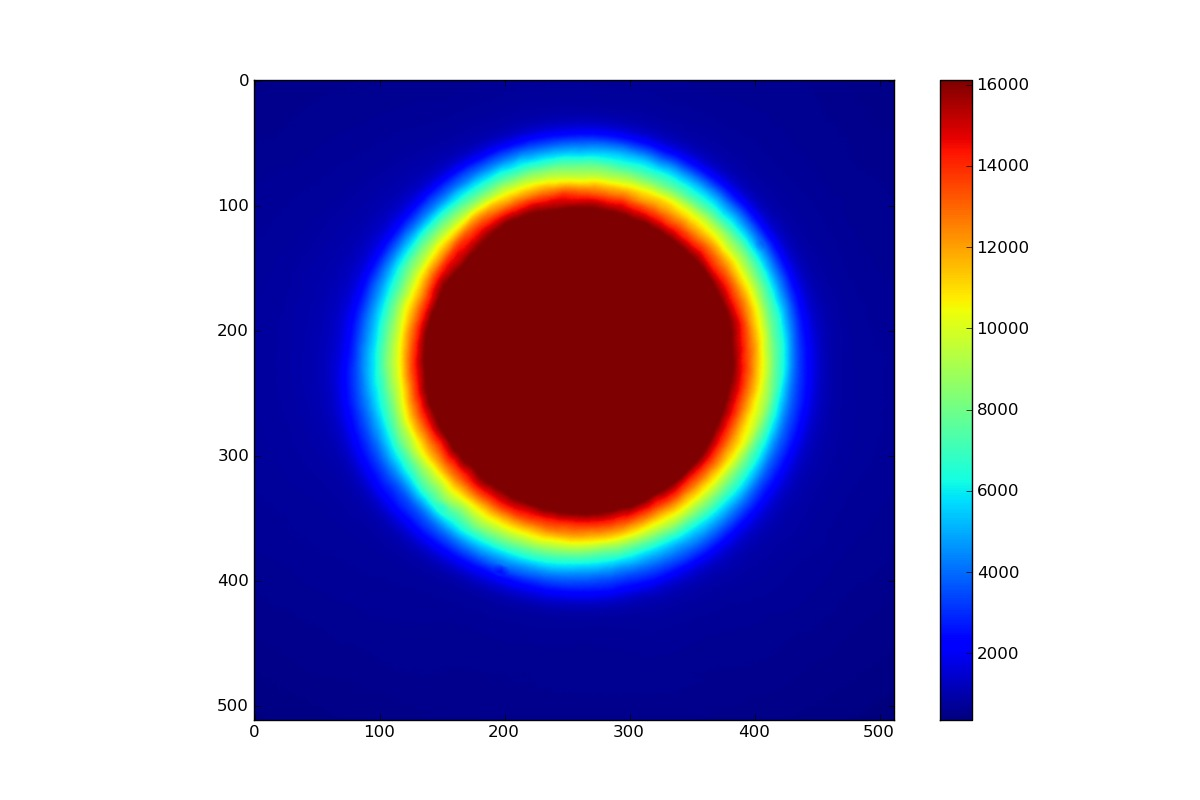
\includegraphics[height=5.9cm, trim=130 10 120 20, clip]{calib-pic}
  \pdfinput{7.4cm, trim=0 0 30 20, clip}{andor_normal_preamp5_exp30}
  \caption{{\bf left:} Image of a defocused area on a fluorescent
    plane sample. This is used for calibrating the detector. {\bf
      right:} Result of a detector calibration. The slope of the curve
    allows to convert the arbitrary analog-to-digital units into
    effective photoelectrons, the point of interception at the $y-$axis
    gives the detector read noise.}
  \label{fig:shot-noise}
\end{figure}
For the calibration of a detector, twenty images of a \cma{detector
  gain calibration} defocused fluorescent object (see left image in
\figref{fig:shot-noise}) are acquired. From the twenty images the
variance of the intensity is determined for each pixel. Then all
occurring intensities are collected into 100 bins. The average
intensity variance of each bin is then plotted against the intensity
(see right image in \figref{fig:shot-noise}). The data lie on a
straight line. From its slope we calculate the gain to convert the
arbitrary analog-to-digital units into the number of effective
photoelectrons. If the data is plotted in this unit, the slope of the
line is one, according to equation \eqref{eq:variance}. The smooth
light distribution in the input images ensures a good coverage for
each data point in the variance-intensity plot and a bit of protection
against drift.

\comment{ % this is just for copying the jpeg file
\jpginput{10cm}{calib-pic}{Image of a defocused area on a fluorescent
  plane sample.}}

To determine the quality of a detector we \cma{measuring read noise}
ensure that no light falls on the detector and create twenty dark
images.  For an ideal, noise-free detector these images would contain
zero everywhere. In a real CCD sensor the variance of the values in
the dark images reflect the readout noise $N_r$ and the mean estimates the offset. Using the calibration
gain, the readout noise can be specified as photoelectrons$/$pixel
($\unit[]{e^-/px}$).

The analysis for the right diagram in \figref{fig:shot-noise} gave a
readout noise of $\unit[5.6]{e^-/px}$. For the evaluation I used the
function \verb!cal_readnoise! of the DIPimage toolbox for Matlab
\citep{Lidke2005a}. In Appendix \ref{sec:python-readnoise-eval} I list
an alternative Python implementation of this algorithm.

The major source for readout noise is the charge amplifier. Its noise is
added uniformly to every image pixel. For readout frequencies above
\unit[1]{MHz} the readout noise increases with the square root of the
read speed \citep{Pawley2006}. Until a decade ago this limited the
readout speed of scientific CCD cameras. Then a new type of sensor was
developed --- the electron-multiplying CCD (EM-CCD) \citep{Mackay}.

This device contains an additional sequence of capacitors (denoted        \cma{electron-multiplying CCD}
multiplication registers), which are operated with a high voltage (up
to \unit[46]{V}). The field accelerates electrons and they can
generate more charge carriers by a process called impact
ionization. This is a statistical process and for every electron going
through a multiplication register, there is an average probability $p$
that it creates another electron. This probability is quite low
($p<1.3\%$) but after a sequence of 536 registers the gain
$M=(1+p)^{536}\approx 1015$ is so high, that even readout noise at \unit[17]{MHz}
readout speed can be neglected.

This amplification process consumes a lot of energy and requires an
elaborate cooling scheme of the detector chip as the gain is
temperature dependent.

Unfortunately, the statistical nature of impact ionization leads to an
uncertainty in gain and therefore introduces a \cma{excess noise
  reduces quantum efficiency} new noise source. As a gain this noise
acts multiplicatively on the signal. \cite{Robbins2003} analyzed the
amplification process and shows that the multiplicative noise, which
is also called excess noise, has the effect of halving the apparent
quantum efficiency of the detector.

Note that for very low light conditions with a minute probability to
detect more than one photon per pixel, the EM-CCD can be run with
maximum gain as a binary detector in photon counting mode. In this
mode the excess noise has no effect whatsoever; but other noise
sources become important.

\newcommand{\SNRid}{\textrm{SNR}_{id}}
\newcommand{\SNRadd}{\textrm{SNR}_{add}}
\newcommand{\SNR}{\textrm{SNR}}
\subsection{Comparison chart for detector selection}
Now I will introduce a comparison chart that I first saw in
\cite{Cameras2012}. It is based on a single equation for the
signal-to-noise ratio $\SNR$ and, if the detector parameters, such as
readout noise and quantum efficiency, are known, a quantitative
estimate of the expected quality of the data can be made.

Shot noise defines the fundamental limit for the signal-to-noise ratio
in photo detectors \citep{Sheppard2006a}. As already mentioned above,
the expected noise for a signal of $S$ photons is $\sqrt{S}$. Assuming
the contributions to a detector pixel are $S$ signal photons, perturbed
by an additional number of $I_b$ photons background light. The
signal-to-noise $\SNRid$ ratio for an ideal, noise-free detector is:
\begin{align}
  \SNRid = \frac{S}{\sqrt{S+I_b}}.
\end{align}
%FIXME wie interpretiert man das bei kleinen S, wenn gauss und poisson
%verteilung nicht gleich aus sehen?

A conventional detector with reduced quantum efficiency $Q_E\in[0,1]$
and additive, Gaussian readout noise with standard deviation $N_r$ (in
$\unit[]{e^-/px}$) can only produce a worse signal-to-noise ratio:
\begin{align}
  \SNRadd = \frac{Q_E\cdot S}{\sqrt{Q_E(S+I_b)+N_r^2}}.
\end{align}
This equation can be adapted for the electron-multiplying CCD. There,
the readout noise is reduced because of the gain $M$ but the influence
of the shot noise is doubled due to the excess noise factor
$F_n=\sqrt{2}$. \nomenclature{$F_n$}{Excess noise factor}
\begin{align}
  \SNR = \frac{Q_E\cdot S}{\sqrt{F_n^2\cdot Q_E \cdot (S+I_b) + (N_r/M)^2}} \label{eq:snr}
\end{align}
This equation permits to compare all the cameras that I can
use for my experiments. Table \ref{tab:cam-param} lists parameters
from their datasheets and the three diagrams in
\figref{fig:camera-snr} shows curves of the relative signal-to-noise
ratio $\SNR/\SNRid$ for three different amounts of background light
$I_b$.

When choosing the parameters I attached particular importance to the
noise performance, even if that comes with a loss in readout speed.

\begin{savenotes}
  \begin{table}[!htbp]
    \centering
    \begin{tabular}{l r r r r r l}
      \toprule
      camera type & $f_\textrm{read}$  & $QE$ & $N_r$ & $F_n$ & $M$ & model \\
       & [MHz] & &  [$e^-/$px] & &  &  \\
      \midrule
      back-thinned CCD & 1 & 0.95 & 5.3 & 1 & 1 &  E2V CCD97\\
      EM-CCD & 1 & 0.95 & 15.0 & $\sqrt{2}$ & 80 & E2V CCD97 \\
      EM-CCD single photon & 17 & 0.95 & 89.0 & 1 & 1000 & E2V CCD97 \\
      sCMOS global shutter& 200 &0.52 & $2.3$ & 1 & 1 & Fairchild CIS2521F\\
      sCMOS rolling shutter& 140 &0.72 & $1.3$ & 1 & 1 & Hamamatsu FL-400\\
      back-thinned sCMOS & --- &0.95 & $0.7$ & 1 & 1 & --- \footnote{Back-thinned sCMOS are not available at the time of writing.} \\
      interline CCD & 20 & 0.62 & 6.5 & 1 & 1 & Sony ICX285\\
      interline CCD & 1 & 0.62 & 2.4 & 1 & 1 & Sony ICX285\\
      \bottomrule
    \end{tabular}
    \caption{Camera parameters for the curves in \figref{fig:camera-snr}.}
    \label{tab:cam-param}
  \end{table}
\end{savenotes}

For a very large number of photons the detector with the highest
quantum efficiency $Q_E$ wins (back-thinned CCD, green line):
\begin{align}
  \lim_{S\rightarrow\infty} \frac{\SNR}{\SNRid} &=
  \frac{\sqrt{Q_E}}{F_n}. \qquad \textrm{(high light limit)}
\end{align}
For detectors with readout noise, there is a number $S_n$ of signal
photons below which the readout noise dominates:
\begin{align}
  S_n&= \frac{N_r^2}{M^2F_n^2 Q_E}-I_b.  \qquad\textrm{(photon shot noise limit)}
\end{align}
I indicate both limits in \figref{fig:camera-snr} using different line
types. The line is dotted in the region where the readout noise
dominates, followed by a thick solid line where both photon shot noise
and readout noise contribute. A thin line indicates the region where
the relative SNR is within 95\% of the high light limit and the
sensor's quantum efficiency becomes the parameter that defines the
performance.

% \gnuplotinput{camera-snr}{Comparison of signal-to-noise ratio for
%   different cameras. Dotted line for lowest light level, where $N_r$
%   is the dominant noise; thin line indicates high light region where
%   quantum efficiency and excess noise factor $F_n$ matter. }

\begin{figure}[!hbt]
  \centering
%  \svginput{1}{camera-snr-svg}
  \pdfinput{14cm}{camera-snr-svg}
  \caption{Comparison of signal-to-noise ratio for
  different cameras. Dotted line for lowest light level, where $N_r$
  is the dominant noise; thin line indicates high light region where
  quantum efficiency and excess noise factor $F_n$ matter.}
  \label{fig:camera-snr}
\end{figure}


The first thing I want to look at is the EM-CCD. For a high gain of
\cma{interpretation of EM-CCD in \figref{fig:camera-snr}} $M=20$ the
curve is horizontal and the sensor differs from the ideal detector
only in terms of a reduced apparent quantum efficiency. In a low
background environment $I_b=0.3$ the electron multiplying mode is only
advantageous for signals with less than 30 photons per pixel. For a
higher background $I_b=30$ electron multiplication does not improve
noise performance --- but note that in this mode the sensor could be
read out at a 10 times higher speed.

In a low background environment and low signal level the EM-CCD comes
very close to the ideal detector, when it is run in photon counting
mode as indicated by the blue-green line in the top left.  In this
case, however, an effect which was neglected in equation
(\ref{eq:snr}) becomes important. The impact ionization which is used
to advantage in the multiplication registers occurs with low
probability during vertical shifts of the signal and thereby adds
approximately $\unit[200]{e^-/frame}$ of spurious charge. This effect
is called clock-induced charge.

Next, I discuss the curves of the active-pixel
sensors. \cma{sCMOS in \figref{fig:camera-snr}}
The device designated as global shutter sCMOS is a sensor with five
transistors per pixel \citep{Vu2011}. Similar to a passive-pixel CCD
sensor this permits to start exposure in all pixels simultaneously,
but it has two major drawbacks. The additional two transistors cover
space that would otherwise be available as light sensitive area and
for quantitative data, a reference frame must be taken for each image,
which increases the readout noise \citep{Gamal2005,Cameras2012}.

% In his Blog Mehta reports something an Andor engineer told him:
% http://blog.mshalin.com/2012/08/global-exposure-with-scientific-cmos.html

The rolling shutter sCMOS sensor has only the minimum three
transistors per pixel and therefore a correspondingly higher quantum
efficiency. For a signal between 6 and 80 electrons per pixel this
sensor provides the best quality at 8 times higher readout speed than
the EM-CCD. Rolling shutter means that the pixel lines are read in
succession but for our prototype it is crucial that all pixels
integrate while the displays show patterns. Fortunately there is a
mode called global exposure synchronization which initiates
integration in the pixels line by line and generates a trigger output
once all pixels have started capturing light. This allows to use the
camera as a master without further effort but the camera can also be
run as a slave. In that case the only requirement is that the trigger
comes early enough ($\unit[10]{ms}$, \cite{Hamamatsu2012}) to initiate exposure in all
lines before the illumination is activated.

% 10-4 Configuring exposure time

The entry back-thinned sCMOS is only a hypothetical sensor which I
added to compare the performance of a low noise active-pixel sensor
with near perfect quantum efficiency.
\subsection{Calibration of the EM-CCD gain}
The method I presented for CCD calibration can be applied to measure
the gain $M$ and the excess noise factor $F_n$ of an EM-CCD. This
requires dark images and image sequences of the smooth intensity
distribution (from the exactly the same sample and illumination) with and without
electron multiplication gain, so that data for both cases can be
converted into detected photoelectrons.

The apparent quantum efficiency with gain is $Q_E/F_n$. Therefore the
excess noise factor can be calculated with
\begin{align}
  F_n =  N_{(1)}/N_{(M)}  
\end{align}
where $N_{(1)}$ and $N_{(M)}$ are the sums of photoelectrons in the
image without and with electron multiplication gain, respectively.

The variance for data without gain is $(\Delta I)^2_{(1)} = Q_E
\langle I \rangle$ and smaller than for data with gain, where the
variance is $(\Delta I)^2_{(M)} = Q_E F_n^2 \langle I \rangle$.

The $x-$axis in the intensity-variance plot is equal to the intensity
for gain-free data and scaled with $M$ for the amplified data.  The
gain $M$ can be calculated from both slopes $m_{(1)}=Q_E$ and $
m_{(M)}=Q_E F_n^2/M$ of the intensity-variance curves:
\begin{align}
  M = F_n^2 \frac{m_{(1)}}{m_{(M)}}.
\end{align}

In Appendix \ref{sec:basic-acquisition} I present code to
automatically measure data for this calibration. In order to cover a
large span of gains, I capture a short exposure image before each
measurement and use the longest exposure time that is possible without
overexposing the sensor.


% - effects to look out for

% - signal pickup fft of dark image to see periodic offset fluctuations

% - gain fluctuations have multiplicative influence more of a problem for scmos

% - not clear how frequent recalibration will be required


% - heating during read can lead to offset drift

% - make sure all the charge is transported out

% - light source brightness fluctuation

% - room light


% - Higher gains are possible but limit the dynamic range.

% - maximum charge handling capacity with linear response: 400000 \citep{2004e2v}


% - cic is a problem

% - thermal effects lead to generation of charge in a ccd

% - for long integration times dark current must be prevented by deep cooling (needs vacuum)


% - clock-induced charge for very fast frame rates


% % cascade II /mnt/backup/safe-with-time/torben/safed/y2009/0414
% % andor ultra ~/1114  python code for calibration and andor basic for acquisition


% - stable light source

% The top left diagram of \figref{fig:ixon} contains such a 2D
% histogram. It was obtained by conventional readout at \unit[3]{MHz} of
% our Andor IXon3 camera (head: DU-897D-CS0-\#BV). The variances are
% collected in 64 intensity bins and their averages are plotted as red
% crosses. The blue line is the result of a linear fit to the first
% $60\%$ of the red crosses. Its slope gives the real gain of the camera
% that can be used to convert ADU into photoelectrons (here
% \unit[1.32]{$e/$ADU}).

% The following figures show corresponding measurements using the EM
% readout mode with varying EM-gain. It is followed by one last
% measurement with conventional readout to verify, that the fluorophores
% did not bleach too much during the experiment.

% The camera was cooled to \unit[$-75$]{$\,^{\circ}{\rm C}$}. In order
% to prevent overexposure of the sensor a preliminary image with a short
% integration time of \unit[10]{ms} was acquired. Then, using this
% image, the integration time was for the experiment was set such that a
% maximum of \unit[10000]{ADU} would occur (in the function
% \textsf{$\sim$GetSaturationExposure}). An internal shutter in the camera
% was closed (\textsf{SetShutter}) to obtain the dark images. The process
% was automated using an Andor Solis Basic program which is listed
% below.


Table~\ref{tab:ixon-table} summarizes the calibration results. The
average of the dark images (in ADU) is given in the column
\textsf{offset}. The read noise in conventional mode is approximately
8 electrons per pixel rms. The column \textsf{mean'} (primed variable)
contains the average number of photoelectrons per pixel in the
illuminated image normalized by the integration time. The rows
\textsf{conv1} and \textsf{conv2} with conventional readout (without
EM-gain) contain approximately the same number. This proves that no
significant bleaching occurred during the experiment.

\subsection{Conclusion}

In this section I discussed how various camera sensors work. I have
explained photon shot noise, which follows from the quantum mechanical
nature of light and so far constitutes a fundamental limit of light
detection. Based on this, I explained a calibration method that helps
to evaluate camera performance and, maybe more relevant for this work,
allows to compare images that were created with different microscopes.

Since low-noise active-pixel cameras became available only late during
my project, and the first models still had some issues --- unstable
software or in the case of the Hamamatsu Orca Flash~2.8 too few
outputs for trigger signals, I designed my system for EM-CCD.  For
most experiments, however, I used an interline CCD.



% The EM-gain process introduces multiplicative noise in the signal. Its
% effect on the photoelectron statistics is the same as lowering the
% quantum efficiency of the sensor. Dividing values of the column
% \textsf{ mean'} from EM readouts by the same value from the
% conventional readout gives the \emph{excess noise factor}\todo{get
%   this right: should be $\sqrt{2}$}. Its value is smaller than one and
% describes the apparent reduction of the quantum efficiency.


% Due to a bug in the capturing process the images in the second row
% (for EM-gain 40) was overexposed and the data should not be used.  Also
% the last experiment \textsf{conv2} with conventional readout reports
% a larger gain of \unit[1.6]{e/ADU} than the first experiment
% \textsf{conv1} with gain \unit[1.3]{e/ADU}. Later we learned that one
% should allow several seconds of settling time, when changing the
% EM-gain voltage. This might explain the difference in gains, even
% though one would think that the conventional readout should be
% decoupled.






% \begin{figure}
%   \centering
%   \pdfinput{7.4cm}{andor_normal_preamp5_exp30}
%   \pdfinput{7.4cm}{andor_emgain100_preamp5_exp30}
%   \pdfinput{7.4cm}{cascade_exp400ms_normal}
%   \pdfinput{7.4cm}{cascade_exp400ms_gain3000}
%   % \includegraphics[width=7cm]{../app_cam/cascade_normal_preamp3_exp30}
%   \caption{{\bf top:} Andor IXon2 {\bf left:} Normal readout with
%     preamp 5 and \unit[1]{MHz} readout rate.  {\bf top right:} EM-gain
%     100 preamp 5. {\bf bottom:} Cascade II {\bf left:} Normal readout
%     at \unit[5]{MHz} $\textsf{mean}=\unit[254.82]{e/pixel}$. {\bf
%       right:} EM-gain 3000 at \unit[10]{MHz},
%     $\textsf{mean}=\unit[122.08]{e/pixel}$, therefore the excess noise
%     factor is 0.48.}
%   \label{fig:old-cams}
% \end{figure}

% sushi 20090414 maybe check for readout speed of cascade II and the
% excess noise factor of the andor

% check in lab book for exact specs of andor ixon2


% \subsection{sCMOS}
% pixel in
% ccd ist passiv
% cmos ist aktiv

% column parallel readout sony exmor

% exmor r additionally back illuminated (only works for small sensors)


% - typically two rolling shutters

% - global shutter increases read noise by a factor of 1.41

% - non-destructive read

% - dual amplifiers enable good low signal performance but high full
% well capacity at the same time at the expense of non-uniform gain

% \citep{Breakthrough2009}

%%% Local Variables: 
%%% mode: latex
%%% TeX-master: "kielhorn_memi"
%%% eval: (reftex-mode)
%%% eval: (flyspell-mode)
%%% End:
 

\chapter{Methods of controlling illumination patterns}
\label{sec:illum-patterns}
\subsection{2-photon laser scanning fluorescence microscopy}
\label{sec:2-photon}
If the laser intensity in the focal spot of a confocal microscope is
sufficiently high, then two infrared photons can be absorbed within
\unit[$\sim 5$]{fs} and excite the same electronic state.

In this regime, the fluorescence emission increases quadratically with
laser intensity. This non-linearity confines the excitation volume to
the vincinity of the focal plane \citep{Denk1990}. Fluorophores
outside of this region are not excited. Therefore this method produces
sectioned images by default and there is no need for a detection
pinhole.

As an additional benefit infrared light is scattered less than visible
light of half the wavelength. This increases penetration depth and
image quality. Photodamage outside of the focal volume is unlikely and
phototoxicity is much lower, compared to the single-photon confocal
microscope, when $z-$stacks are acquired.

However, the phototoxicity within the focal volume is higher and
techniques like ultramicroskopy (section
\ref{sec:light-sheet-microscopy}) with single-photon excitation are
preferable, when low overall phototoxicity is a requirement.

\section{programmable array}
\cite{Caarls2011}
\comment{
\jpginput{}{led-array}{}
\jpginput{}{myholo}{}
\jpginput{}{phase}{}
\jpginput{}{tf-gpc}{}
%\jpginput{}{dunsby}{}
%\jpginput{}{aod}{}
}

\chapter{Methods for controlling illumination patterns}
\label{sec:approaches}
\nomenclature{CLEM}{Controlled light exposure microscopy}%
\begin{summary}
  This chapter provides an overview of current methods of fluorescence
  microscopy that allow to produce a controlled distribution of the
  excitation light. I focus in particular on the techniques that prevent
  unnecessary illumination of out-of-focus structures and reduce
  phototoxicity.
\end{summary}
\section{Light sheet fluorescence microscopy}
\label{sec:light-sheet-microscopy}
\begin{summary}
  Light sheets can be directly created with separate optics to
  illuminate the sample from an orthogonal direction. Another
  promising method to create a sheet is to use a high numerical
  aperture objective near the total internal reflection angle. There
  is a trade-off between the sheet width and the field of view because
  both of these things are interrelated due to diffraction.
\end{summary}
The idea of illuminating a sample from the side dates back quite far
into the history of microscopy. Already one hundred years ago, an
additional objective, arranged perpendicular to the detection
objective, was used for illumination of the focal plane in the
specimen. This dark field technique was used to characterize gold nano
particles in gold ruby glass \citep{Siedentopf1903}.

Eventually, this illumination method was also applied for fluorescence
microscopy. First, it was used to analyze cochlea specimen
\citep{Voie1993} and, more recently, for the development of embryos
\citep{Huisken2004}. Results in the latter paper have sparked interest
in the technique at many labs \citep{Santi2011}.
\subsection{Light sheet generation with cylindrical lens}
\begin{figure}[!hbt]
  \centering
  \svginput{1}{spim-sketch}
  \caption{Schematic of SPIM (selective plane illumination
    microscope). A cylindrical lens illuminates the specimen with a
    thin sheet of light along the focal plane of the
    objective. Rotating the sample and/or moving it along the axis
    allows reconstruction of a sectioned three-dimensional volume of
    the fluorophore concentration with improved light utilization
    compared to conventional microscopes \citep[inspired
      by][]{Huisken2004}.}
  \label{fig:spim}
\end{figure}
\figref{fig:spim} shows how the light sheet can be focused into the
specimen using a cylindrical lens. \cite{Huisken2004} employ a water
dipping objective with long working distance (\unit[1\ldots 2]{mm})
and comparatively low NA for detection. A $10\times$ objective with
$\unit[660]{\mu m}$ field of view diameter is used with a sheet
thickness that varies less than $42\%$ ($\unit[6\ldots 8]{\mu
  m}$). The light sheet not only improves sectioning and contrast, but
also increases the axial resolution from originally $\unit[14]{\mu m}$
by nearly a factor of two.

\nomenclature{SPIM}{Selective plane illumination microscopy}

The axial resolution of detection objectives with higher numerical
aperture isn't improved so easily over an extended field of
view. Shading effects, diffraction and refraction can deteriorate the
light sheet. As an improvement of the technique it was suggested to
rotate the specimen or illuminate with multiple sheets of light from
different directions.

A major difference between this technique and more conventional
microscopy techniques is the way the sample is mounted. In a normal
microscope, usually, a specimen is placed with a drop of embedding
medium on a \unit[170]{$\mu$m} thick cover slip. Then it is flipped
onto a microscope slide and sealed with nail varnish. This approach of
mounting the sample does not work for an ultramicroscope because there
the sample has to be accessed from two perpendicular sides. Often the
specimen are embedded in an agarose cylinder or sometimes, they are
fixed in a liquid--filled chamber.

\subsection{Light sheet generation using the detection objective}
\label{sec:hilo}
\begin{figure}[!hbt]
  \centering
%  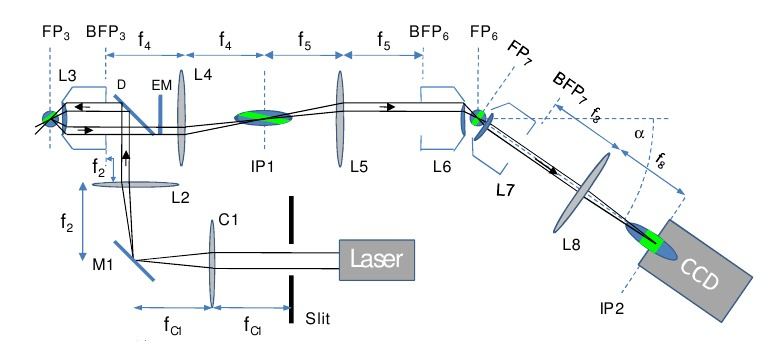
\includegraphics[width=12cm]{dunsby}
  \svginput{1}{dunsby-redraw}
  \caption{Schematic of oblique plane microscopy (OPM). An index
    matched sample is excited using an oblique plane of light. The
    illuminated plane is tilted relative to the focal plane
    FP1. Therefore, out-of-focus fluorophores on the periphery of the
    field of view are excited as well. Two additional objectives in
    the detection path are used to reconstruct an aberration free
    image of all the excited fluorophores (drawing inspired by
    \cite{Dunsby2008}).}
  \label{fig:dunsby}
\end{figure}
Modern high numerical aperture objectives allow to illuminate an
\emph{index matched} sample with a half angle of up to
$70^\circ$. This enables illumination of an oblique and thin sheet of
light in the specimen just as in selective plane illumination
microscopy. However this technique (oblique plane microscopy, OPM) has
the advantage, that only one objective is used and therefore it will
work with conventional microscope slides. However, one difficulty is
that some of the excited fluorophores are severely defocused in the
intermediate image plane (plane IP1 in \figref{fig:dunsby}). Dunsby
describes how to rotate the observational plane optically in order to
recover an aplanatic image from the oblique illumination plane
\citep{Dunsby2008}. For this, they re-image the sample through two
additional objectives.

\nomenclature{OPM}{Oblique plane microscopy.}

\begin{figure}[!hbt]
  \centering
  \svginput{1}{hilo-sketch}
  \caption{Schematic of rays in HILO (highly inclined and laminated
    optical sheet) technique. The specimen is embedded in a medium of
    lower optical density than the immersion medium. For a very high
    illumination angle --- corresponding to a point on the periphery
    of the back focal plane --- the light would be reflected at the
    ``cover slip-medium'' interface due to the total internal reflection
    (TIR). For HILO, a point on the back focal plane slightly closer
    to the optic axis is illuminated. The light enters the embedding
    medium at a highly inclined angle and only a thin sheet in the
    focal plane is illuminated \citep[inspired by][]{Tokunaga2008}.}
  \label{fig:hilo}
  % FIXME the construction of the rays is not correct, they should go
  % to the principal plane and then should be just axially shifted
  % into the aplanatic sphere.
\end{figure}


\nomenclature{TIR}{Total internatl reflection.}

Biological specimen are often not index matched and have a lower index
$n_e\approx 1.33\ldots1.45$ than the immersion oil $n=1.52$. As
indicated in \figref{fig:hilo}, the refraction at the interface
between cover slip glass and embedding medium can be exploited to
illuminate the specimen with a light sheet that is nearly parallel to
the focal plane.  This technique is called highly inclined and
laminated optical sheet microscopy (HILO) \citep{Tokunaga2008,
  Konopka2008}.

\nomenclature{HILO}{Technique for microscopy illumination: highly
  inclined and laminated optical sheet}

Note that the index mismatch between embedding and immersion medium
will introduce aberrations (mostly spherical) in the detection which
will limit the useful imaging depth to a few microns for high aperture
lenses.
\section{Scanning techniques with improved light utilization}
\begin{summary}
  A confocal microscope exposes out-of-focus fluorophores with
  approximately the same dose as the in-focus fluorophores when
  producing and image of a focal slice. During acquisition of z-stacks
  this results in bleaching and successive slice contain less and less
  signal. In particular living organisms may be harmed due to
  phototoxicity during the observation.

  Here I present two methods that can mitigate this effect. The first
  method is two-photon microscopy, in which the excitation is limited
  to the focal plane.

  Furthermore, there is controlled light exposure microscopy that
  selectively illuminates the sample depending on its structure. It
  delivers images with the overall quality as a conventional confocal
  while decreasing phototoxicity and bleaching considerably.

  This method is based on a feedback that controls excitation dose
  depending on the local fluorophore concentration and therefore
  benefits from any latency improvements. In this context I discuss
  two approaches that can increase the scanning speed considerably.
\end{summary}
\subsection{Two-photon laser scanning fluorescence microscopy}
\label{sec:2-photon}
If the laser intensity in the focal spot of a confocal microscope is
sufficiently high, then two infrared photons can be absorbed within
\unit[$\sim 5$]{fs} and excite the same electronic state.

In this regime, the fluorescence emission increases quadratically with
laser intensity \citep{goppert1931elementarakte}. This non-linearity
confines the excitation volume to the vincinity of the focal plane
\citep{Denk1990}. Fluorophores outside of this region are not
excited. Therefore this method produces sectioned images by default
and there is no need for a detection pinhole.

As an additional benefit infrared light is scattered less than visible
light of half the wavelength. This increases penetration depth and
image quality. Photodamage outside of the focal volume is unlikely and
phototoxicity is much lower, compared to the single-photon confocal
microscope, when $z-$stacks are acquired.

However, the phototoxicity within the focal volume is higher and
techniques like ultramicroscopy (section
\ref{sec:light-sheet-microscopy}) with single-photon excitation are
preferable, when low overall phototoxicity is a requirement.
\subsection{Controlled light exposure microscopy (CLEM)}
\label{sec:CLEM}
In the confocal microscope the excitation beam is scanned in a
rectangular grid over the focal plane. Normally this is done using two
galvanometer mirrors, one of which addresses pixel columns and the
other (much slower) addresses the rows. The excitation laser is
continuously active during a scan over one line. So ultimately, the
integration time at the detector defines horizontal sampling.
\begin{figure}[hbtp]
  \centering
  \svginput{1}{clem-sketch}
  \caption{Illustration of a typical fluorescence image
    of a neuronal cell and histograms for three different regions. In
    the conventional confocal microscope areas without fluorophores
    (A) and the areas with many fluorophores (C) are subjected to an
    unnecessarily high light dose. Controlled light exposure
    microscopy (CLEM) adapts the illumination to the sample in order
    to reduce phototoxicity and bleaching.}
  \label{fig:clem}
\end{figure}

The measured signal in each pixel is proportional to the collected
photons and therefore subject to Poisson distributed quantum shot
noise (see section \ref{sec:photon-noise}). Thus, the signal-to-noise
radio fluctuates over the image. The image is particularly noisy in
areas with low fluorophore concentration. For the human observer and
many computer algorithms the noise in these particularly noisy areas
defines the image quality. The fact that areas with more signal have
considerably less noise does not increase the perceived image quality,
neither does it improve the results of an edge detector for the dim
areas. Considering the detrimental effects of the excitation light it
would be advantageous to acquire fluorescence images with constant
signal-to-noise ratio in each pixel.



This approach is pursued in the controlled light exposure microscope
(CLEM). It utilizes a confocal microscope, adapted for fast switching
of the excitation light. Depending on whether the photons collected
during a short preparation time, each pixel is classified into one of
three classes. The darkest pixels (class A in \figref{fig:clem}) are
assumed to not contain any information and the laser is switched off
for the remainder of the dwell-time. Pixels with moderately many
photons (class B) are illuminated for the entire dwell-time. For
pixels with a high fluorophore concentration (class A) the excitation
laser is turned off, once a certain number of photons have been
detected. In this case the signal is not the number of photons but the
illumination duration.

In this way, one obtains a picture in which bright regions have a
constant signal-to-noise ratio and regions without fluorophores are
illuminated with only a small dose. Especially when capturing z-stacks
this procedure significantly reduces phototoxicity and photobleaching
--- with an insignificant decline in image quality.

%  Unfortunately, due to the photon nature of
% light, sometimes a region of type (B) is incorrectly classified as (A)
% which introduces dark pixel artifacts in the image \citep{Hoebe2010}.

The CLEM approach was first presented by Hoebe et al.\ in 2007,
followed by an independent similar version with adaptive control of
the laser power for 2-photon microscopy by Chu et al.\
\citep{Hoebe2007,Chu2007}.

% FIXME i'm not sure if 2007 was first publication
\subsection{Fast beam steering}
In a conventional confocal microscope, the beam is steered by two
galvanometer mirrors. While this technique offers very good light
throughput the inertia of the mirrors limit the access rate of spots
in the focal plane. The CLEM technique could be simplified and
improved by an inertia-free solution to steer the excitation beam from
pixel to pixel. The laser intensity would no longer have to be
modulated and when enough photons were collected in a pixel, the next
one could be addressed.

The z-focus is often controlled by piezomechanical elements that
either move the sample or the objective, i.e.\ objects of relatively
large mass. Therefore, the settling time for focus movements has a
correspondingly large latency and focusing is often much slower than
lateral pixel access.

\subsubsection{Acousto-optic deflectors for fast beam steering}
An interesting alternative to galvanometric mirrors are acousto
optical deflectors (AODs). They consist of a transparent optical
element into which an acoustic wave is coupled by means of an
ultrasound transducer.  An acoustic wave is a longitudinal variation
of the interatomic distance and thereby affects the local electron
density and thus the refractive index of the medium. An acoustic wave
in an AOD allows diffracting a beam of light with moderate efficiency
(70\%). By changing the acoustic frequency the angle of diffraction
can be controlled. Due to its strong chromatic aberration and low
efficiency, an AOD should not be used to descan the beam of a normal
confocal microscope. However, this device is well suited for a
two-photon microscope, where descanning is not strictly necessary.  In
\cite{Otsu2008} the authors achieved a switching time of $\unit[4]{\mu
  s}$ using an acoustic wave in tellurium dioxide (TeO$_2$).

\begin{figure}[htbp]
  \centering
  \svginput{1}{reddy-redraw}
  \caption{Schematic of an acousto-optic deflector (AOD) illumination
    system with $z-$focusing. Drawing inspired by \citet{Reddy2008}}
% in focusing single s highly preferred http://www.future-perfect.co.uk/grammartips/grammar-tip-focussed-focused.asp
  \label{fig:aod}
\end{figure}

\nomenclature{AOD}{Acousto-optic deflector}
\nomenclature{AOM}{Acousto-optic modulator}

The system in \cite{Reddy2008} even uses an acousto optic technique to
focus the excitation beam of a two-photon microscope (see
\figref{fig:aod}). A pair of two ultrasound transducers (e.g. X1 and
XZ in the figure) produce two counter-propagating waves with
continuously changing frequency. The resulting diffraction pattern
resembles an one-dimensional Fresnel zone --- oscillations of high
frequency on the outside and low frequencies towards the center. A
combination of two such elements but rotated by 90 degrees allows
focusing the beam, similar to how two cylindrical lenses would (see
\figref{fig:aod}).

\subsubsection{Aberration-free optical refocusing}
Achieving the resolution limit of modern microscope objectives using
acousto-optic Fresnel zones seems impossible or at least very
difficult. An alternative approach that can significantly speed up
conventional focusing techniques is based on a similar technique as
the oblique plane microscope (see section \ref{sec:hilo}). In
\cite{Botcherby2007} and \cite{botcherby2012aberration} an additional
objective produces an unmagnified three-dimensional image of the
sample which allows rapid refocusing with a lightweight mirror. This
approach is achromatic and can focus many tens of microns deep into
the sample while maintaining diffraction limited resolution. Unlike
the acousto-optic device this method is not limited to a single
collimated beam and can be applied in widefield microscopes.

\section{Non-scanning techniques}
\subsection{Intensity modulation}
\subsubsection{Programmable array microscopy}
\label{sec:pam}
The main element of the programmable array microscope is a digital
micro mirror (DMD). It is placed into the intermediate image and acts
simultaneously in the excitation as well as the detection beam
path. The mirrors can be programmed to have one of two
deflections. Either they send light into the sample or they send it
into a beam dump. This allows structured illumination with a
computationally defined pattern. In the simplest case, when only a
single pixel is turned on, the operation of the PAM resembles that of
a confocal microscope. Fluorescence light of in-focus fluorophores
returns to the micro mirror that was responsible for the excitation and
is directed towards the camera~1. Out-of-focus fluorescence will be
reflected by any of the other DMD mirrors and ends up on camera 2.

\begin{figure}[htbp]
  \centering
  \svginput{1}{pam-sketch}
  \caption{Schematic of a programmable array microscope (PAM)
    \citep[inspired by][]{Verveer1998}. A digital micro mirror
    device (DMD) containing an array of tiltable mirrors is imaged
    into the focal plane of the objective. Returning fluorescent light
    from out-of-focus fluorophores is distributed onto both
    cameras. In-focus fluorescence is only imaged onto the camera 1.}
  \label{fig:pam-sketch}
\end{figure}


At the time when \cite{Heintzmann2001a} was written, EM-CCDs were not
widely available. In order to reduce the effects of readout noise,
cameras~1 and 2 integrate for a long time while the DMD displays many
patterns. The pattern sequence could for example be a single pixel
which scans the entire field. This would be very slow, so instead,
patterns of a pseudorandom sequence are presented which significantly
accelerates data acquisition, because each individual pattern excites
more in-focus information. However, at the same time crosstalk is
increased, i.e.\ additional light from out-of-focus fluorophores is
collected in camera 1.  The images from both cameras for z-stack
acquisitions are reconstructed using a maximum likelihood
deconvolution.

A technique similar to controlled light exposure microscopy (CLEM,
section \ref{sec:CLEM}) has been implemented in a programmable array
microscope (PAM) \citep{Caarls2011}. 


There are a few drawbacks with the programmable array microscope.
First, diffraction losses at the DMD reduce detection
efficiency. Second, if excitation light causes fluorescence or Raman
scattering at the DMD surface, it is impossible to distinguish this
disturbance from the fluorescence signal of the sample. Third, it is
difficult to align the optics such that DMD pixels are imaged exactly
and without distortion on camera pixels.

Distorted imaging could be retrospectively corrected by
interpolation. However, this process would destroy the known noise
characteristics of the sample values. The values in an interpolated
image are no longer Poisson distributed and application of the maximum
likelihood estimation is problematic.

With the availability of cameras with sub-electron readout noise
(EM-CCD or sCMOS) one would no longer place the DMD in the detection
path. Instead, one could acquire an image of each individual pattern
and do the descanning computationally.


\nomenclature{PAM}{Programmable array microscopy}%
\nomenclature{DMD}{Digital micro mirror device}%
\nomenclature{MLE-PAM}{Minimized light exposure programmable array microscope}%
\subsection{Direct illumination}
An obvious method for doing spatial control is to image a
two-dimensional array of high-power micro-LEDs into the specimen.
\begin{figure}[hbtp]
  \centering
 % 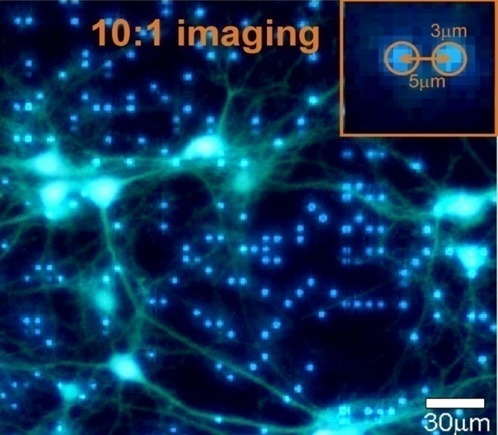
\includegraphics[width=7cm]{led-array} 
  \svginput{1}{cell-drawing}
  \caption{Schematic of a micro-LED illumination array and the outline
    of a neuronal cell, inspired by \citet{grossman2010}.}
  \label{fig:led-array}
\end{figure}
However, the problem is to achieve sufficient \emph{irradiance} and
\emph{fill factor}. The angular emission profile of LEDs is often
Lambertian, i.e.\ the back focal plane of the objective would be
over-illuminated and a lot of light would be lost. The fill factor is
limited because it is difficult to put a lot of LEDs close to each
other.  The technique has been demonstrated using a $64\times64$ array
of $\unit[20]{\mu m}$ micro-emitters with $\unit[50]{\mu m}$ pitch
\citep{grossman2010} (see \figref{fig:led-array}).  The LEDs can be switched at millisecond speed
and emit at a wavelength of $\unit[(470\pm22)]{nm}$.

\nomenclature{GFP}{Green fluorescent protein}
\nomenclature{EGFP}{Enhanced green fluorescent protein}
\nomenclature{YFP}{Yellow fluorescent protein}
\nomenclature{VCSEL}{Vertical-cavity surface-emitting laser}
\nomenclature{LED}{Light emitting diode} % Fixme
\nomenclature{MMA}{Micro mirror array}
\nomenclature{LCoS}{Liquid crystal on silicon (display)}
\nomenclature{DPSS}{Diode-pumped solid-state (laser)}

Currently it is not clear whether direct illumination will ever
replace the more flexible spatial light modulators. Manufacturers of
direct illumination devices will optimize their technology for
consumer applications such as mobile phone displays, where neither fill
factor nor extreme radiant intensity (\unit[]{W/sr}) are very
important.  Arrays of Vertical-cavity surface-emitting lasers (VCSEL)
may become interesting alternatives to LED-arrays because they can
provide high radiant intensity, but currently they are not readily
available in the interesting wavelength ranges.


\subsubsection{Light field microscopy}
\label{sec:light-field-microscopy}
Interesting work on light fields originally started in the macroscopic
domain of cameras \citep{Lippmann1908} %,Sokolov1911 
and was eventually
applied as a technique for microscopy
\citep{Levoy2006,Levoy2009,Zhang2009}. This approach is built on
imaging through an array of microlenses.
\begin{figure}[!hbt]
  \centering
  \svginput{1}{microlens-levoy-sketch}
  \caption{Schematic of microlenses in the intermediate image plane
    \citep[inspired by][]{Levoy2006}. A spatial intensity modulator
    is illuminated from the right with an extended light
    source. Groups of neighboring pixels downstream of individual
    microlenses are imaged into the pupil. Therefore these pixels
    allow to control the irradiance in the sample at the area that is
    conjugated to the microlens. }
  \label{fig:microlens-levoy-sketch}
\end{figure}


Downstream of the microlenses a spatial light modulator (SLM) is
placed, so that a rectangular group, of say $10\times 10$ pixels is
imaged into the pupil. Each microlens illuminates the pupil from
another angle. In \cite{Levoy2009} they use an intensity SLM and each
of its pixels controls the radiant intensity (\unit[]{W/sr}) in the
area of the sample that is covered by the conjugated image of the
corresponding microlens. A trade-off has to be made between the
resolution that can be obtained in the pupil and the resolution in the
focal plane in the sample. The latter is limited by the size of the
microlenses.

The paper uses microlenses in the detection path as well. The camera
captures a lot of images of the pupil. This allows retrospective
refocusing or rotation of the image using the ray-based plenoptic
theory. However, splitting the images with microlenses has severe
drawbacks and should not be used with fluorescence microscopy. When
recording camera images, important phase information is lost and the
sub-images can not be recombined to obtain the full resolution of the
microscope objective.

In the case of illumination the loss in resolution is not as important
and perhaps the full resolution could even be maintained when a phase
SLM is used. % FIXME rainer fragen
\nomenclature{TL}{tube lens}
\subsection{Temporal focusing}
\begin{figure}[!hbt]
  \centering
  \svginput{1}{temporal-focus-sketch}
  \caption{Schematic of temporal focusing \citep[inspired
    by][]{Oron2005}. A grating in the intermediate image plane
    separates the pulse into its spectral components. The out-of-focus
    areas of the specimen are illuminated with a longer pulse. Only in
    the focal plane, all spectral components interfere coherently and
    form a short intensive pulse.}
  \label{fig:oron}
\end{figure}
The axial extent of ultra-short laser pulses can be as thin as a few
microns. A collimated beam can be split into different spectral
components by a grating in the intermediate image plane
\citep{Oron2005}. The tube lens focuses the diffraction pattern into a
line in the back focal plane of the objective.

The objective, which has to be corrected for chromatic aberration and
dispersion, then focuses all the beams onto the focal plane. Different
spectral components arrive in the focal plane at the same time. The
out-of-focus points see an extended illumination. For a high NA
objective, a pulse duration of $\tau=\unit[20]{fs}$ results in slice
of $z\approx\tau c/2\approx\unit[3]{\mu m}$ thickness around the
focus, where the beam has significant intensity.

Using this technique it is possible to build a widefield 2-photon
microscope that only excites fluorophores within the focal plane. The
technique can be further improved by spatially modulating the beam in
the intermediate image plane for CLEM like performance. This technique
has been implemented in the TF-GPC approach and will be discussed in
the next section.

\subsection{Phase modulation}
\subsubsection{Digital holography}
Certain types of liquid crystal spatial light modulators can be used
to modify the phase of light. When such a device is placed into the
back focal plane of a lens, it is possible to control the light
distribution in its front focal plane. An iterative algorithm
(iterative Fourier transform algorithm, IFTA) can be used to establish
a phase image on the liquid crystal display that will result in an
intensity distribution in front of the lens.

\begin{figure}[htbp]
  \centering
  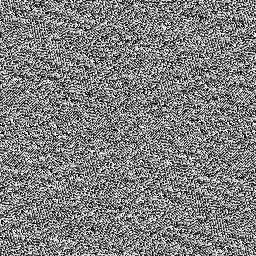
\includegraphics{myholo}\quad
  \svginput{1}{phase-holo_my} 
  \caption{Schematic of spatial illumination by phase holography. A
    phase-only SLM displays a hologram in the plane $P'$ which is
    conjugated to the back focal plane $P$ of the objective
    \citetext{inspired by slide from V. Emiliani}.}
  \label{fig:phase-holo}
\end{figure}


\nomenclature{IFTA}{Iterative Fourier transform algorithm}

This approach has been used to excite a two-dimensional pattern in the
specimen \citep{Lutz2008,Zahid2010} and is advantageous especially for
cases where only small parts of the specimen ought to be
illuminated. As opposed to conventional intensity spatial light
modulators, the light can be redirected from dark areas into the
bright areas.

% single photon 405nm uncaging, ifta,
% spherical wave approximation
There is also a limited possibility to create three-dimensional
patterns, e.g.\ several points below, in and above the focal plane by
displaying Fresnel zone planes.  For illumination, usually a laser
with non-zero interference length is employed. However, this
illumination contains an unwanted ``speckle'' pattern in the form of
noisy non-uniformities. To a certain extent, the contrast of the
speckle pattern can be reduced by controlling spatial and temporal
coherence of the illumination (sweeping the frequency of the laser or
changing illumination direction while the detector is integrating).

Holographic control can be used with 2-photon excitation as well
\citep{Nikolenko2008}, % two photon
but this exacerbates the effect of speckles.
\subsubsection{Generalized phase contrast (GPC)}
\begin{figure}[htbp]
  \centering
%  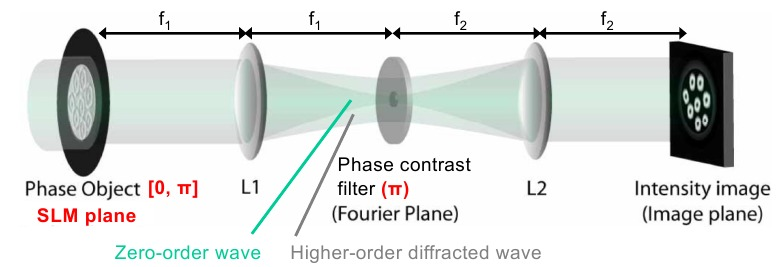
\includegraphics[width=12cm]{phase} % FIXME redraw
  \svginput{1}{rodrigo}
  \caption{Schematic of generalized phase contrast
    \citep[from][]{Rodrigo2008}.}
  \label{fig:phase}
\end{figure}
A phase contrast microscope objective \todo{modified ?} can be used to
convert a phase image from the intermediate image plane into an
intensity image in the specimen \citep{Rodrigo2008}\todo{read more of
  this}. Compared to digital holography, hardly any computation is
necessary. Yet, the phase spatial light modulator can concentrate a
lot of light on a small region of the specimen as opposed to other
techniques, which involve intensity modulation and lose all the light
of dark areas by sending it into a beam block or something similar.

The generalized phase contrast method is suitable even with spatially
incoherent illumination\todo{slightly ?}. However, when the
fill-factor -- the size of the bright area in the image -- changes,
the phase contrast filter must be changed.
\subsubsection{Generalized phase contrast and temporal focusing (TF-GPC)}
The combination of generalized phase contrast and temporal focusing
allows spatially controlled illumination of in-focus areas
\citep{Papagiakoumou2010}. Usage of a phase spatial light modulator
results in high light efficiency compared to intensity modulation.
Splitting and recombination of the spectral components of the pulse
reduce speckle noise considerably.
\begin{figure}[htbp]
  \centering
%  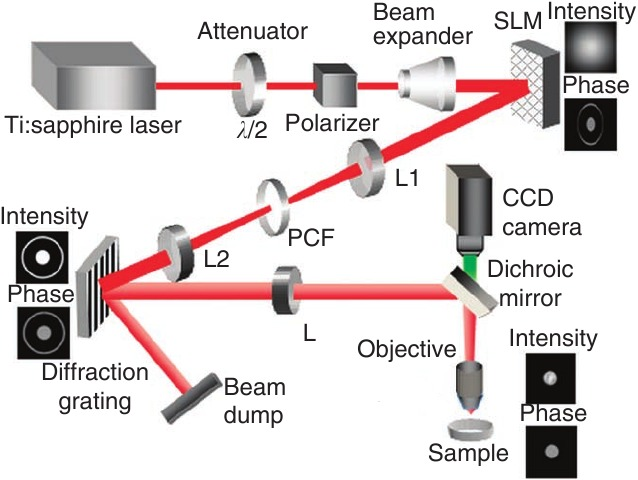
\includegraphics[width=10cm]{tf-gpc} 
  \svginput{1}{papa}
  \caption{Schematic of phase contrast with temporal focusing (TF-GPC)
    \citep[inspired by][]{Papagiakoumou2010}, PCF is a phase contrast filter.}
  \label{fig:tf-gpc}
\end{figure}
\nomenclature{PCF}{Phase contrast filter}


%%% Local Variables: 
%%% mode: latex
%%% TeX-master: "kielhorn_memi"
%%% eval: (reftex-mode)
%%% eval: (flyspell-mode)
%%% End: 

\chapter{The concept of spatio-angular microscopy}
\label{sec:concept}
\begin{summary}
  Here I introduce the spatio-angular microscope. First I explain the
  concept of its illumination system using exemplary fluorophore
  distributions, that occur in typical specimen.

  Then I describe some decisions we faced during the initial design
  phase concerning the arrangement of optical components. Furthermore,
  I position our method among known approaches of light control for
  microscopy. Of all published techniques for excitation illumination
  control, the light field microscope \citep{Levoy2006} comes closest
  to our approach.  I explain differences between both techniques and
  discuss their respective pros and cons.  I address the peculiarities
  and limitations of the hardware components in chapters
  \ref{sec:dev1} (optics) and \ref{sec:mma} (micromirror based pupil
  plane SLM).  Initially, the details would be detrimental to clarity.

  The effective use of the spatio-angular microscope, requires more
  knowledge about the specimen than a conventional or a SPIM
  microscope \citep{Huisken2004}. Ideally, the distribution of
  refractive index and fluorophores in the specimen should be
  known. If these parameters were precisely known, there would be no
  need for an image in the first place. However, while imaging a known
  specimen, sufficiently good predictions of these parameters can
  often be made. The higher the accuracy of these prognoses, the
  greater the reduction in phototoxicity will be.

  The computer-based selection of appropriate illumination masks
  requires the prediction, or at least an approximate estimation, of
  the three-dimensional distribution of light in the specimen.

  In the last part of this chapter, I describe the computational
  control loop in our spatio-angular
  microscope and touch topics of image processing.
\end{summary}
\section{Motivation}
In order to introduce the basic idea underlying the spatio-angular
microscope, I consider the distribution of excitation light in the
object of a conventional fluorescence microscope:
\figref{fig:hourglass-all}~a) schematically illustrates the side view
of the excitation beam path through objective lens and object in a
confocal microscope. A parallel beam with a circular cross-section
(this cross-section is not shown in the illustration) passes through
the lens. The lens focuses the light in its focal plane.

Between lens and focal plane the light rays form a convergent circular
cone. If refractive index variations in the object are negligible, the
light distribution below the plane of focus forms a cone as well, due
to symmetry.  Assuming a non- or weakly absorbing specimen, the energy
of the light in the circular cross-sections of the cone remains
constant\footnote{The ray-model is valid in large parts of
\figref{fig:hourglass-all}~a), but not everywhere. The Law of
Malus--Lupin states that rays and wavefronts are equivalent as long as
rays do not intersect (caustic), or (FIXME formulas?) a strong
intensity gradient occurs. Thus the ray-model is valid almost
everywhere in the cone, except for a region with a distance of a few
wavelengths to the edge, and the focus itself. While the wave-optical
treatment of these areas is possible, it is computationally much more
expensive than ray tracing. Wave-optical effects either lead to
blurring in a length scale of a few wavelengths or intensity
fluctuations due to interference. If necessary, we can use heuristics
to find an upper bound for the local intensity from ray tracing
results. For this reason we exclusively employ the ray-model in this
work.}\label{sec:ray-valid}.


The fluorescent bead (1), in the focus, would therefore be excited
significantly more than the bead (2) outside the focal plane. Also
shown is the light distribution in the intermediate image plane.

The image of the in-focus bead (1) is sharp, i.e.\ its emanating  % FIXME i need confocal here
fluorescence light is concentrated on an area as small as possible and
positioned exactly on the detection pinhole. Conversely, the image of
the out-of-focus bead (2) is blurred and its fluorescence light is
distributed over a large area.

While only a tiny proportion of the light emitted by the out-of-focus
bead contributes to the detection signal of the confocal
microscope---and therefore hardly affects the image quality, with
respect to overall phototoxicity of the full confocal system---it
would be better to prevent the excitation of the out-of-focus bead in
the first place.

\begin{figure}[!hbt] \centering \svginput{.43}{hourglass-all}
  \caption{{\bf (a)} Two fluorescent beads are illuminated by all
angles that the objective can 
deliver. The sharp image of the in-focus bead is deteriorated by
blurry fluorescence of the out-of-focus bead (2). {\bf (b)} Angular
control allows selective illumination of the in-focus bead (3), and
results in a better image on the camera. {\bf (c)} Angular control,
however, is insufficient, when an extended in-focus area is
illuminated. {\bf (d)} Then, simultaneous spatial and angular control
allows sequential excitation of the in-focus beads, while excluding
the out-of-focus bead (10).}
  \label{fig:hourglass-all}
\end{figure}

The scheme in \figref{fig:hourglass-all}~b) demonstrates how the light
cone would have to be manipulated in order to exclude the out-of-focus
bead (4). The expected fluorescence image in the intermediate image
plane then contains only information from the in-focus bead (3).

Viewed from the in-focus bead (3) the change in illumination
corresponds to a restriction of the light angles. Such control can be
exerted well through a mask in the other focal plane of the objective
lens (also denoted back focal plane or pupil plane).

Thus it is useful and possible to equip a confocal microscope with
angular control. However, in our project we set out to to build a wide
field microscope in order to benefit from the speed and quantum
efficiency of modern cameras.

I now turn to the task of bringing angular control to the wide field
microscope. \figref{fig:hourglass-all}~c) shows a configuration of the
specimen with two in-focus beads (5) and (6), and one out-of-focus
bead (7).  The angular illumination control is ineffective for this
arrangement of beads.  If both in-focus beads, (5) and (6), are
exposed simultaneously, i.e.\ an extended light source illuminates the
entire field, then the out-of-focus bead (7) is always excited.

Only by separate illumination of the in-focus beads (8) and (9), as
shown in \figref{fig:hourglass-all}~d), angular control regains its
function. For this reason a wide field system with angular control,
using a mask in the pupil, requires an additional mask conjugate to
the field.  Therefore, we call our method spatio-angular
microscopy. ``Spatial'' refers to the illumination control in the
field and ``angular'' refers to the control in the pupil plane.

% FIXME 2012 khodjakov schilling

\begin{figure}[!hbt] \centering \svginput{1.5}{memi-simple}
  \caption{Simplified schematic of the illumination system in our
spatio-angular microscope. A homogeneous extended light source
delivers light from the left. It is imaged by lenses $L_1$ and $L_2$
into the intermediate image $F'$. Then the tubelens $L_3$ and the
objective $L_4$ form an image of $F'$ in the sample plane $F$. We use
two spatial light modulators (SLM) to control the spatial and angular
light distribution in the specimen---the focal plane SLM in F', and
the pupil plane SLM in P'.}
  \label{fig:memi-simple}
\end{figure}

\figref{fig:memi-simple} shows the optical path through our prototype
in a simplified form.  From the left side, an extended light source
illuminates the system. A sequence of telecentric lenses $L_1$, $L_2$,
$L_3$ and the objective lens $L_4$ image the light source from F''
into the front focal plane (indicated by F, for field). The etendue
(see page \pageref{sec:etendue} for its definition) of the light
source must be large enough to simultaneously fill both, the pupil P
as well as the field F.

In each of the two planes P' and F' we place a spatial light modulator
(SLM) that allows to control the intensity of the transmitted light.

Looking at the scheme in \figref{fig:memi-simple}, one might argue
that we could save a lens, if we placed the pupil plane SLM into P
instead of P'. There are three reasons why this is neither possible,
nor beneficial: First, the pupil of modern high-performance objective
lenses is typically not accessible. Second, the detection path for
fluorescent light should contain as few optical components as possible
and we can definitely not afford it to be blocked by a SLM.  Third,
the two masks induce non-linear, and therefore difficult to predict,
filtering of spatial frequencies. An analysis requires consideration
of partial spatial coherence, but it should be clear (FIXME) that only
the downstream\footnote{Downstream regarding the propagation direction
  of the excitation light.} SLM will always deliver a good image,
mostly independent of the state of the SLM upstream.

Considering the fact that the image of the focal plane SLM is most
important to us, we decided to place it downstream of the pupil plane
SLM. The focal plane SLM may disturb the image of the pupil plane SLM
in P, but we can always produce very fine, high-contrast structures in
the sample F.

The abiltity to achieve high resolution in the field is the main
difference between our approach and Levoys light field microscope.  In
the light field microscope, the density of the microlenses noticeably
limits the resolution. As opposed to our system, the light field
microscope allows to control the angle of incidence in all field
positions independently.  But, additionally to the reduced focal plane
resolution, this requires a single high-resolution SLM with a
comparatively low refresh rate. We use two small SLMs, which can each
achieve \unit[1]{kHz} frame rate and enable interesting experiments,
e.g.\ optogenetic control of neuron activities.

Furthermore, structured illumination with high resolution patterns
allows us to circumvent the missing cone problem of the widefield
microscope.  Later I will show that depth discrimination improves with
higher resolution patterns (FIXME ref).
\section{An imaging protocol with spatio-angular illumination control}
\subsection{Description of an exemplary biological specimen} 
I now refer to the \celegans\ test sample for phototoxicity that I
introduced in section \ref{sec:intro-phototoxicity}. So far I did not
reach the point of being able to image the development of a real
embryo. Key problems are the low light throughput of the illumination
system and the length of time necessary to update images on the focal
plane display. Nevertheless, I always kept this example in mind while
I was developing the control software for our microscope.

During the first few hours, the embryo develops confined within the
constant volume of its egg, which has an ellipsoidal shape, extends 40
to 60 microns and can be readily observed using a $63\times$ objective
lens. Cell divisions occur every few minutes.  During development the
nuclei get smaller and more dense. In order to track the fate of all
individual cells it is sufficient, to capture one stack per minute
with 41 layers and a $z-$step of 1~micron.
\subsection{Preparation of living embryo samples} 
For an experiment a hermaphrodite worm is cut and the embryos are
placed on an agarose pad, so that they stay immobile during
imaging. This procedure is explained\footnote{Note that
  \cite{Murray2006} describes an improvement of this protocol that
  prevents squeezing the embryos too much.} in \cite{Hope1999}. Of
these embryos, the experimentor chooses a young specimen, that has not
yet divided. We avoid to use fluorescence excitation for this step.
The undivided embryos can be distinguished using the less phototoxic
differential interference contrast (DIC) imaging mode.

\subsection{Sectioning through structured illumination} 
To get an estimate of the initial distribution of the fluorophores in
the embryo I obtain the very first stack with structured illumination
and no angular control. I use this method to avoid the missing cone
problem of the widefield microscope. Perhaps for our particular task
of finding the position of one nucleus within the egg, widefield
images would be just sufficient.  However, for our spatio-angular
method, knowledge about the fluorophore distribution is very important
and therefore we built our microscope such that we can obtain optical
sections.

We compared conventional structured illumination using max$-$min
(FIXME) reconstruction with laser and LED illumination. Although LED
illumination resulted in excellent optical sections, the
reconstruction of laser illuminated images contained artifacts.

% {\color{red} - (FIXME muss das vielleicht in appendix?) In einem
% ersten Entwicklungsschritt, bevor InVision uns den Prototyp fuer das
% spatio-angulare Mikroskop zur Verfuegung stellte, setzten wir einen
% SLM in die Zwischenbildebene. Auf dem SLM wurden vier Streifenmuster
% angezeigt und Wir verglichen einen 70mW 473nm DPSS laser mit 470nm LED
% Beleuchtung (CoolLED).}

Therefore, we decided to implement HiLo (see Appendix FIXME). With
this algorithm, we obtain artifact-free optical sections, regardless
of the illumination source. As another advantage the HiLo method
increases acquisition speed, because only two raw images per slice are
necessary.


% {\color{red} wir haben artefakte in der max-min rekonstruktion
% beobachtet, wenn wir ein grobes streifenmuster (8 forthdd slm pixel
% periode) mit laser beleuchtet haben

%      - irgendwann hat rainer das erklaert aber ich kann mich nicht
% mehr dran erinnern aber es waere cool, wenn ich die story bringen
% koennte
     
% - grobes gitter heisst im amplitudenbild: einige ordnungen (nicht nur
% 3) gehen durch die bfp

%      - irgendwie kam es dadurch im intensitaetsbild zu einigen hoehere
% ordnungstermen

%      - bei LED (extended source) werden die weggemittelt, bei laser
% nicht

%        - ein bisschen kopfzerbrechen bereitet mir noch der bias

%        - im paper habe ich das nicht verstanden [2011 mertz Optically
% sectioned in vivo imaging with speckle illumination HiLo microscopy]

%        - aber ich habe ihr java imagej plugin decompiliert bekommen
% und koennte versuchen ihre implementierung zu verstehen (andererseits
% ist mir das jetzt ziemlich egal)

%        - unter equation 10: The first two terms are variance
% contributions of shot noise. Filtering has the effect of reducing
% noise variance and is taken into account with the integral term. This
% bias must thus be subtracted from $\sigma^2$ prior to the evaluation
% of C. We have also not considered the effects of pixelation in the CCD
% camera. If the pixel size is non-negligible ..  }

\subsection{Computer model for the integration of a priori knowledge
about the biological events} 
Given an initial measurement of the fluorophore distribution of the
embryo, I employ a computational algorithm to find good illumination
conditions for subsequent stack acquisitions. An important requirement
is that the computer can estimate, which areas of the sample should be
protected from illumination.

For our test system, the \celegans\ embryo, it is a promising approach
to represent its three-dimensional fluorophore distribution by a
simple model: Spheres encompassing the nuclei, indicate regions with
fluorophores. When in focus, the spheres are the source of useful,
informative fluorescence signal, but should be protected against
exposure when out of focus.

As I mentioned earlier, there are also unused histones with
fluorophores outside of the nuclei. The images reveal that they occur
in the cytoplasm at a much lower concentration than in the
nuclei. Fluorophores in the cytoplasm have a smaller phototoxic
effect, because any radicals they produce are much less likely to
reach the DNA and therefore inflict substantially less damage.  In the
following my goal is to protect only out-of-focus nuclei from
exposure. The regions in between are used to bring the light in.


During observation, the nuclei, i.e.\ the centers of the spheres, move
slowly within the embryo. For small periods of time we can describe
this movement using a vector field of growth velocities.

A cell division announces itself by a change of the fluorophore
distribution of the nucleus due to chromatin condensation and spindle
formation. Therefore, whenever the computer detects such changes in
the images, in one of the following time steps an additional sphere
should be introduced to account for the new daughter cell.

So far I have implemented a simple algorithm, to convert a time series
of image volumes from a confocal microscope into a sphere model
\citep{Santella2010}.  One of our project partners (Jean-Yves Tinevez,
http://fiji.sc/wiki/index.php/TrackMate) developed a more
sophisticated plug-in for ImageJ, that provides the lineage tree and
snapshots of the developing cells (see \figref{fig:trackmate}).
\begin{figure}[!hbt] \centering
  \pdfinput{6cm}{TrackMate_Celegans_lineage}
  % trim=left bottom right top
  \qquad
  \includegraphics[trim=25cm 0cm 84cm 87cm, clip, height=5cm]{TrackMate_Celegans_lineage_vector}
  \caption{ A detail of a lineage tree visualized in TrackScheme. An
    image of each nucleus is shown in each time step. Note the
    elongated structure of the nucleus before the cell division
    event.}
  \label{fig:trackmate}
\end{figure} Before our microscope can be used for our biological
problem, the computer model has to be extended so that it reliably
tracks the movement of nuclei.  Overlooking any nucleus would prevent
this nucleus from being imaged in later acquisitions and would be a
setback for the experiment.  Estimating the vector field of growth
velocities helps to track nuclei more robustly and allows to predict
their positions for the next exposure.

Currently we have not implemented programs that would fulfill the
requirements for imaging a developing embryo.  However, in the
following text I assume that the described position predictions were
available and I discuss how I determine masks for the focal plane and
pupil plane SLM.

\cite{Murray2006}

TODO FIXME Bernhard Kauslers work is nice
\verb!http://archiv.ub.uni-heidelberg.de/volltextserver/11820/1/thesis_fkaster.pdf!
Live-cell microscopy image analysis for the study of zebrafish embryogenesis
\verb!http://hci.iwr.uni-heidelberg.de/publications/mip/techrep/kausler_12_discrete.pdf!
A Discrete Chain Graph Model for
  3d+t Cell Tracking with High
    Misdetection Robustness

(FIXME read this)


\subsection{Illumination optimization by means of raytracing} 
I now discuss a method to find both SLM masks for image acquisitions
with minimal phototoxicity. First I define a mask for the focal plane
SLM:

From the predicted arrangement of spheres we select in-focus nuclei by
intersecting the model with a planar surface. I then define focal
plane SLM masks to selectively illuminate each of the in-focus nuclei,
by drawing a bright disk in the appropriate position.

Based on such a mask, we can determine which angles can illuminate the
in-focus target nucleus, without exposing out-of-focus nuclei.

As I already explained at the beginning of this chapter on page
\pageref{sec:ray-valid}, ray-optical theory suffices to describe the
light distribution within the sample.

I connect the periphery of an out-of-focus nucleus with a point inside
the in-focus target. This defines a circular cone of rays, that are
propagated through the objective lens. Their intersection with the
pupil plane results in a figure that still very much resembles a
circle---I found that already seven rays lead to good representation
of its perimeter.  An algorithm computes these figures for every
out-of-focus nucleus and for a few in-focus targets points within the
bright areas of the focal plane pattern. In this manner I construct
the desired mask for the pupil plane SLM.

In order to trace the rays into the pupil, I need the design
parameters of the objective lens (vertex position, curvature and
material for all surfaces). Unfortunately, these rarely are publicly
available for high-performance objective lenses. Nevertheless, in
chapter (FIXME) I use a simpler model of the objective lens, that
requires only three parameters: focal length, refractive index of the
immersion medium and numerical aperture. These are always known.

Additionally, I have adapted the model for non-index-matched embedding
of the specimen. This problem occurs when the embryo is illuminated
with an oil immersion objective, using HILO (FIXME ref). It should be
noted, however, that good image quality of the embryo can only be
achieved with an objective lens that has the same immersion index as
the embryo. Otherwise data from 20 microns within the sample will be
severely deteriorated by spherical aberrations.

\chapter{Device 1: prototype for spatio-angular illumination}


\begin{figure}[!htbp]
  \centering
  \svginput{2}{memi-real}
  \caption{Schematic of the light path through our microscope. Laser
    light enters from the lower left, is scrambled and homogenized to
    illuminate the full MMA and LCoS. $F$ is the field plane in the
    sample and its primed versions are conjugated planes. $P$ is the
    pupil of the objective. $B_0$ and $B_1$ are adjustable circular
    apertures. PBS is a polarizing beam splitter. DBS is a dichromatic
    beam splitter.}
  \label{fig:memi-real}
\end{figure}

\begin{figure}[!htbp]
   \centering
   \svginput{2}{memi-sketch}
   \caption{Schematic of the lenses in the MEMI system and their focal
     lengths. The focal length $f_\textrm{TL}$ of the tube lens can be
     varied. This allows to scale the second intermediate image
     $r''_\textrm{MMA}$ of the micro mirror array to fit the back
     focal plane of different objectives. Dimensions in mm.}
   \label{fig:memi-sketch}
 \end{figure}

\jpginput{14cm}{setup-photo-blueprint}{The wide field epi-fluorescence
  microscope with attached illumination head. The positions of the two
  spatial light modulators (Micro mirror array (MMA) and liquid
  crystal on silicon display (LCoS)) are indicated. Drawing by Josef
  Wenisch (In-Vision, Austria).}

% \imagw{14cm}{mma}{{\bf left:} Scanning electron microscope image of
%   the micro-mirror array (MMA).  The pixel pitch of the device is
%   \unit[0.016]{mm}. The hinges for the tilt movement and the
%   electrodes are clearly visible. {\bf middle:} Optical reflective
%   microscope image of the MMA. {\bf right:} exaggerated rendering of
%   how a 8x8 checker board pattern would be displayed on the
%   device. Electron and optical micrograph by Fraunhofer IPMS Dresden
%   (Germany)}

% \begin{figure}[!hbt]
%   \centering
%   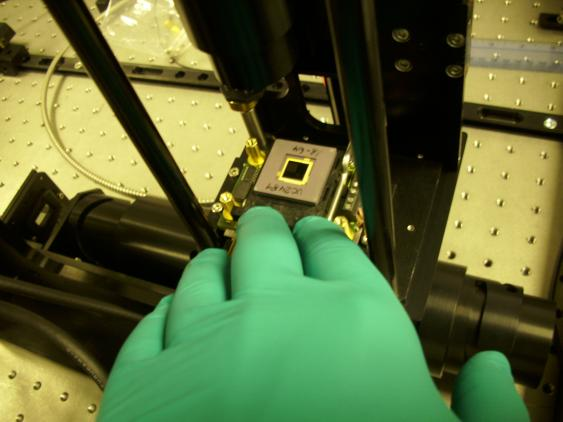
\includegraphics[width=7cm]{mma-plain}
%   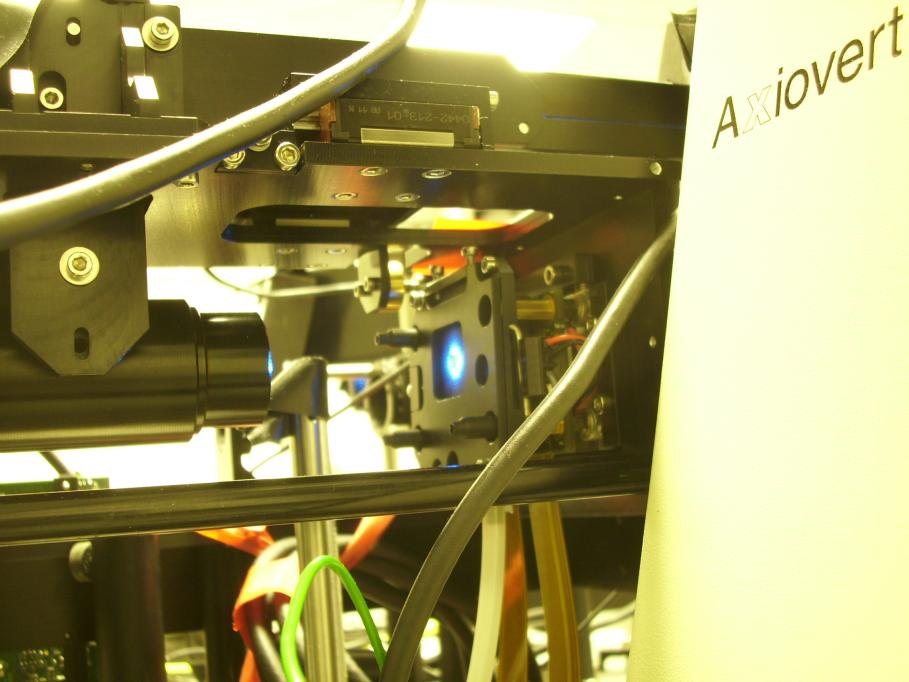
\includegraphics[width=7cm]{mma-ill}
%   \caption{{\bf left:} Micro mirror array chip during installation of
%     the optics. {\bf right:}~Illuminated micro mirror array in the
%     aligned system.}
%   \label{fig:mma-closeup}
% \end{figure}

%\chapter{optimization of the spatio-angular illumination patterns}
%\label{sec:optimization}
%\chapter{mma as an intensity modulator}
%\label{sec:mma}
%\include{mma}
%\include{device2}
% ~/from-hp2-notebook/0331/lens
% there is also code
\chapter{Raytracing for spatio-angular microscopy}
\label{sec:raytrace}
\renewcommand{\i}{\nvect i}
\begin{summary}
  Imaging with the microscope we developed requires a continuous
  update of the patterns for the spatial light modulators during
  operation. It is not easily possible to solve the problem with
  commercial software. Therefore, a simple raytracer is implemented in
  this work.

  This chapter documents the basic concepts. Some approximations,
  which are usually used in optical design (paraxial, only non-skew
  rays) are not applicable here, because rays are to be pursued in all
  possible angles through diverse fluorophore distributions in the
  specimen.

  I begin by introducing simple geometric formulas to determine the
  points of intersection between a ray and a plane or a sphere. I also
  describe how to calculate refraction at a planar surface.

  Then I explain the refraction at a thin, paraxial lens and show a
  modification of the formulas for high aperture lenses. This allows
  to trace rays through a microscope objective in two directions
  (denoted as detection or illumination direction) without knowing the
  exact design parameters and glass types.

  Furthermore, I consider the refraction at the ``cover slip--medium''
  interface for non-index matched media. This enables the calculation
  of illumination patterns for highly inclined and laminated optical
  sheet microscopy, as introduced in section \ref{sec:hilo}.

  I follow up with a rather technical discussion of a geometric
  problem that helps to significantly speed up the raytracing
  calculations for the specific case of a sample that can be
  represented as a three-dimensional distribution of fluorescent
  spheres.

  {\bf Note:} The formulas that are emphasized by surrounding frames
  are implemented in the computer code that is published on
  \url{https://github.com/plops/mma/tree/master/lens}.
\end{summary}
\section{Basic geometric algorithms}
\subsection{Intersection of a ray and a plane}
 \begin{figure}[!hbt]
   \centering
   \svginput{1}{plane-intersection}
   \caption{Schematic of plane-ray intersection.}
\end{figure}
Let a ray start at a point $\s$ with direction $\hd$.  A plane
(defined by a point $\c$ and the unit normal $\n$) intersects this ray if
its normal and the ray's direction are not perpendicular:
$\n\,\hd\not=0$. The distance between the plane and the origin is
$h=\c\,\n$. The equation of the plane is given in Hesse normal form:
\begin{align}
  \r\n=h
\end{align}
I replace the coordinate $\r$ with the ray equation and solve for the
parameter $\tau$.
\begin{align}
  (\s+\tau\,\hd)\,\n&=h\\
  \s\n+\tau\,\hd\,\n&=h\\
  \tau&=\boxed{\frac{h-\s\,\n}{\hd\,\n}}
\end{align}
The point of intersection is located on the ray at $\s+\tau\,\hd$.
\subsection{Intersection of a ray and a sphere}
Let a ray start at a point $\s$ with direction $\hd$.  Let a sphere be
centred in $\c$ with radius $R$. There are two equations
\begin{align}
  (\r-\c)^2&=R^2\\
  \r&=\s+\tau\hd
\end{align}
that define the intersection points. By substituting $\r$ one obtains
a quadratic equation in the distance $\tau$ along the ray:
\begin{align}
  (\s+\tau\hd-\c)^2&=R^2\\
  \l&:=\boxed{\s-\c}\\
  l^2+2\tau\l\hd+\tau^2-R^2&=0\\
  \underbrace{1}_a\tau^2+\underbrace{2\l\hd}_b\tau+\underbrace{l^2-R^2}_c&=0
\end{align}
%\subsubsection{Solving the quadratic equation to obtain the ray--sphere intersection}
In order to prevent numerical errors the following solution should be
used \citep{Press1997}:
\begin{align}
  \Delta&:=\boxed{b^2-4ac}\\
  q&:=\boxed{-\frac{b+\sqrt{\Delta}\sign b}{2}}\\
  \tau&=\boxed{
  \begin{cases}
    q/a &\,\textrm{when}\,\abs{q}\approx 0\\ 
    c/q &\,\textrm{when}\,\abs{a}\approx 0\\
    (q/a, c/q) &\,\textrm{else}
  \end{cases}}
\end{align}
If the discriminant $\Delta$ is negative the ray misses the sphere and
there is no solution. If the discriminant is zero the ray touches the
periphery of the sphere and there is only one solution. A positive discriminant
corresponds to two solutions.
\subsection{Refraction at planar surface}
Now I describe the refraction at a planar surface\footnote{I use the
  same notation as \cite{McClain1993}.}. The wavelength of the light
in vacuum defines the length of the wave vector $\k_0$. The lengths of
the incident and transmitted wave vectors $\k_1$ and $\k_2$ are
obtained by multiplication with the refractive index in their
respective half space:
\begin{align}
  k_0&=2\pi/\lambda\\
  k_1&=n_1 k_0\\
  k_2&=n_2 k_0.
\end{align}
\begin{figure}
  \centering
  \svginput{1}{refraction}
  \caption{Refraction at an interface transforms the incident wave
    vector $\k_1$ into the outgoing wave vector $\k_2$.}
  \label{fig:refraction-plane}
\end{figure}
I choose the normal $\n$ to be directed into the half-space of the
incident wave (see \figref{fig:refraction-plane}) and define the
transversal and normal component of the wave vectors to be:
\begin{align}
  \k_{1n}&=(\k_1\n)\n\\ 
  \k_{1t}&=\k_1 - \k_{1n}.
\end{align}
These two vectors are orthogonal and during refraction the transversal
component of the wave vector is invariant:
\begin{align}
  k_2^2&=k_{2n}^2 + k_{2t}^2\\
  \k_{2t}&=\k_{1t}.
\end{align}
Using the two equations from above, one can calculate the length of
the normal component of the transmitted wave vector $\k_2$:
\begin{align}
  k_2^2&=k_{2n}^2 + (\k_1 - \k_{1n})^2\\
  k_{2n}^2&=k_2^2-(\k_1-(\k_1\,\n)\,\n)^2\\
  &= k_2^2-(k_1^2-2(\k_1\,\n)^2+(\k_1\,\n)^2)\\
  &= k_2^2-k_1^2+(\k_1\,\n)^2.
\end{align}
Finally, one can express the full transmitted wave vector $\k_2$ using
only known quantities:
\begin{align}
  \k_2&=\k_{1t}-\sqrt{k_2^2-k_1^2+(\k_1\,\n)^2}\n\\
  &=\k_1-(\k_1\n)\n-\sqrt{k_2^2-k_1^2+(\k_1\,\n)^2}\n. \label{eq:k2}
\end{align}
I divide by $k_2$ with $\k_2/k_2=\t$ and $\k_1/k_2=\eta\,\i$ in order
to introduce unit direction vectors $\i$ and $\t$ for incident and
outgoing light. The relative index change across the interface is
$\eta=n_1/n_2$. With these substitutions equation (\ref{eq:k2}) becomes:
\begin{align}
  \t&=\eta\,\i-\eta\,(\i\,\n)\,\n-\sqrt{1-\eta^2+\eta^2\,(\i\,\n)^2}\,\n\\
  &=\boxed{\eta\,\i-\left(\eta\,\i\,\n+\sqrt{1-\eta^2(1-(\i\,\n)^2)}\right)\n}
\end{align}
When the expression under the square root is negative a reflection
occurs instead  of refraction. Note that in my application total internal
reflection (TIRF) just corresponds to a loss of the beam, because the reflected beam no longer
contributes to sample illumination. The exact direction of this
 beam is not relevant in this case but I give the equation here for
completeness' sake.

In the case of reflection, the tangential component is invariant and
the normal component inverts sign:
 \begin{align}
   \k_2&=\k_{1t}-\k_{1n}\\
   &=\k_1 - 2\k_{1n}\\
   &=\k_1-2(\k_1\,\n)\,\n\\
   \t_\textrm{TIR}&=\boxed{\i-2(\i\,\n)\n}
 \end{align}
\section{Refraction through lenses}
An \cma{validity of thin lens model} ideal lens is infinitesimally
thin and is completely defined by its focal length. For an ideal lens the focal
length is independent of the incidence angle but in practice, the
model of the thin lens is only valid for lenses of long focal length and
for paraxial rays that subtend very small angles from the optical
axis.

For a better approximation of refraction through a \cma{principal planes} thick lens
the two principal planes of
the thick lens are calculated and the ray is shifted between them axially
\citep{Smith2000}. The principal plane of a thick lens is located on
the intersection between an incident beam $\i$, that is parallel to
the optical axis, and the transmitted beam $\r$. Just as the focal
length, the principal planes are a property of lenses that are only
defined in the paraxial limit. There are always two principal planes,
one for each of the two possible illumination directions. The
distances between each principal plane and its corresponding focus
point (the intersection of $\r$ with the optical axis) are identical,
and define the focal length.

As already mentioned in section \ref{aplanatic} on page
\pageref{aplanatic} a microscope objective is a lens which is
corrected to have a constant focal length for rays of widely varying
incidence angle. In this case, the principle surface is no longer a
plane but is deformed into a spherical surface. After introducing the
formulas for the thin lens in the next section, I show in section
\ref{sec:high-aperture-lens} how to carry over those formulas to a
model that describes an aplanatic lens with immersion.

\subsection{Refraction through a paraxial thin lens}
First I describe the refraction by a thin lens: The incident beam with
direction $\i$ hits the lens at the point $\vrho$. A line parallel to
$\i$ through the centre $O$ of the lens defines the point on the focal
plane, which will be intersected by the transmitted ray $\r$ as well.


\begin{figure}[hbtp]
  \centering
  \svginput{1}{lens-fwd}
  \caption{Construction of a ray that is refracted through a thin
    lens. The incident beam with direction $\i$ (from right) hits the
    lens at the point $\vrho$. This diagram is inspired from a figure
    in \cite{Hwang2008}.}
\end{figure}


The red triangle~1 with the points $ABC$ is similar to green
triangle~2 with points $FOA$. All three angles are identical because
each of the lines are parallel: $\overline{CB} \parallel
\overline{OA} \parallel \vrho$, $\overline{FA} \parallel
\overline{CA}$ and $\overline{AB} \parallel \overline{OF} \parallel
\i$. The side $\overline{OF}$ is hypotenuse of the yellow right angled
triangle 3. Its adjacent with respect to the angle $\theta$ has length
$f$. Therefore one can deduce the length
$\abs{\overline{OF}}=f/\cos\theta$.



Between the two similar triangles, the following relation 
can be used to calculate the length $\abs{\overline{BC}}$:
\begin{align}
  \frac{\abs{\overline{BC}}}{\abs{\overline{BA}}}&=
  \frac{\abs{\overline{OA}}}{\abs{\overline{OF}}}\\
  \frac{\abs{\overline{CB}}}{1}&=
  \frac{\rho}{f/\cos(\theta)}.
\end{align}
Given its length, the vector $\vv{CB}$ is now calculated by its length
and the direction $\vrho$. With this vector and $\i$ one can now
obtain the (arbitrarily scaled) transmitted vector $\r'$.  Only the
two framed equations need to be implemented to calculate refraction on
a thin lens with the procedure from above:
\begin{align}
  \vrho&=(x_0,y_0,0)^T=\rho (\cos\phi,\sin\phi,0)^T\\
  \phi&=\arctan(y_0/x_0)\\
  \cos\theta&=\boxed{\i\,\hz}\\
  \r'&=\i- \frac{\cos\theta}{f}\vrho\\
  \r&=\boxed{\frac{f}{\cos\theta} \i -\vrho}
\end{align}
with the axial unit vector $\hz=(0,0,1)^T$.
\subsection{Refraction through high aperture objective (illumination)}
\label{sec:high-aperture-lens}
Now I modify the results of the calculation from the previous section
to treat an aplanatic immersion objective \citep{Hwang2008}.
\begin{figure}[!hbt]
  \centering
  \svginput{1}{obj-fwd}
  \caption{Ray construction for a high numerical aperture objective
    with immersion. As opposed to a thin air lens the objective's
    focal length needs to be corrected by the focus difference vector
    $\a$ to accommodate for the immersion and one must take into
    account spherical principal surface (aplanatic surface).}
\end{figure}
I account for the immersion medium by axially shifting the focal plane
in sample space to $nf$ using the difference vector $\a$, i.e.\ in an
immersion medium with $n=1.52$ the focus moves further away from the
principal plane.
\begin{align}
  \a &= \boxed{f (n-1) \hz} \\
  R &= \boxed{nf}
\end{align}
In order to account for the curvature of the aplanatic surface, the
origin of the transmitted ray is axially shifted by a $\rho-$dependent
sag $\s$ from the principal plane onto the aplanatic surface:
\begin{align}
  \s &= \left(R - \sqrt{R^2-\rho^2}\right) \hz
\end{align}
The final ray exiting the objective has the direction $\r_0$:
\begin{align}
  \r_0 &= \boxed{\r + \a - \s}.
\end{align}

All microscope lenses that come into consideration for use in the
system that we built are designed as an aplanatic lens. The model described by above
formulas is therefore very well suited to represent the objectives
when we run our illumination optimization algorithm to find
illumination patterns for the two SLM in our spatio-angular
microscope.

In the paper \citet{Hwang2008} the authors demonstrate the viability
of this model by comparing its results with a full raytrace through a
$100\times$ objective with $NA=1.4$. There, focus displacement errors
are less than \unit[130]{nm} for a field of $\unit[86.4]{\mu m}$
radius. This is perfectly adequate for our application.

One might think it would be better to know the exact objective
parameters, i.e.\ glasses, curvatures and vertex positions of lens
surfaces. These details are, however, to my knowledge not published by
any manufacturer. In addition alignment of the components plays a
prominent role in building high performance objectives. Therefore just
the design parameters alone probably do not provide a better model of
a microscope objective. They would have to be augmented with
performance measurements of the individual objective,
e.g. point-spread functions in different regions of the field.

\subsection{Reverse path through oil objective (detection)}
Now I consider an oil immersion objective in the detection direction,
tracing rays from the sample into the pupil.

For that I present two approaches. The first and simpler one utilizes
the fact that a perfect microscope lens converts ray angle in the
sample in a linear manner into positions on the pupil. This approach
is sufficient when calculating pupil plane SLM patterns for samples in
an index matched embedding medium.

In the second approach I additionally calculate the angle in which
rays emerge from the pupil. For a perfectly aplanatic lens this would
hardly be an advantage but the formulas will be modified to take into
account aberrations.
\subsubsection{Easy case: back focal plane positions only}
If the points of ray intersection of the back focal plane are
sufficient, a full raytrace is not necessary. This is the case with
aberration-free imaging, i.e.\ when the sample is embedded in an index
matched medium and we want to calculate a pattern for the pupil plane
SLM. Then it is possible to ignore the starting points of rays in the
specimen and just work with their directions.

A unit ray direction $\i=(x,y,z)^T$ in sample space is transformed
into a position $\r_b=(x',y')^T$ in the back focal plane of the
objective. The azimuthal angle $\phi$ isn't changed when going through
the objective. The polar angle $\theta$ defines how far off axis the
back focal plane is hit.
\begin{align}
  \phi'&=\phi=\arctan(y/x)\\
  \theta&=\arcsin(\sqrt{x'^2+y'^2})\\
  \r_b&=r_b\,(\cos\phi',\sin\phi')^T,\quad\textrm{with}\   r_b=nf\sin\theta
\end{align}
 \begin{figure}[!hbt]
   \centering
   \svginput{1}{obj-rev}
   \caption{Schematic for tracing a ray direction $\i$ from sample
     space into the back focal plane. The bigger the angle between
     $\i$ and the optical axis, the further outside the ray will pass
     through the back focal plane.}
 \end{figure}
 \subsubsection{Full raytrace through oil objective in detection
   direction}
\label{sec:objective-raytrace-detection}
Now I discuss the general case and calculate both the origin and the
direction of a ray emerging from the back focal plane. This is
necessary in order to trace light bundles from the specimen into the
plane of the camera (or focal plane SLM). In the next section I will
further modify these formulas to incorporate aberrations due to
non-index matched embedding medium.

The position of the objective is defined by its principal point $\c$
and the normal $\n$ (directed along optical axis towards sample
space). The incident ray is defined by its starting point $\p$ and the
direction $\i$. First I calculate the centre of the aplanatic sphere
$\vect g$ (see \figref{fig:obj-rev-full}).
\begin{align}
  \vect g &= \c + nf\, \n.
\end{align}
\begin{figure}[!htbp]
  \centering
  \svginput{1}{obj-rev-full}
  \caption{Construction to find the transmitted ray through an oil
    immersion objective from a point within the sample.}
  \label{fig:obj-rev-full}
\end{figure}
Then I obtain the position $\p'$ by intersecting the incident ray and
the plane perpendicular to the optical axis through the centre
$\vect{g}$ of the aplanatic sphere.  The focus difference vector $\a$ is
defined by its length and the optical axis. It can be used to
calculate an intermediate point $\p''$.
\begin{align}
  \a &= -f\, (n-1)\,\n \\
  \p'' &= \p' + a.
\end{align}
The point $\p''$ has been shifted, so that an aplanatic air lens would
image it exactly as the oil objective would image $\p'$. One can use
$\p''$ to find the direction $\t$ of the transmitted ray. It is just
the normalized difference vector $\vect m$ to the principal point $\c$.
\begin{align}
  \vect m &= \c - \p'' \\
  \t &= \vect m / \abs{\vect m}.
\end{align}
As a last step I calculate the starting point $\e'$ of the transmitted
ray by intersecting the incident ray with the aplanatic sphere (in
point $\e$) and axially shifting this point onto the principal plane.

Note: In order to verify the correctness of these formulas or their
implementation it is possible to compare the algorithms of this
section (for tracing in detection direction) and section
\ref{sec:high-aperture-lens} (for illumination direction).
\subsection{Treatment of aberration (detection)}
\label{sec:ray-aberration}
Now I will extend the formulas of the previous section to include
aberrations due to a non-matched embedding medium $n_e\not=n$.

I consider a ray originating in point $\p$ with direction $\i$ within
an embedding medium of index $n_e$. I determine the intersection $\f$
of the ray with the ``cover slip--embedding'' interface and refract to
obtain $\i'$. Then I calculate the time $t$ a photon takes, to travel
from $\p$ to the interface $\f$:
\begin{align}
  t = \abs{\f - \p} \frac{n_e}{c}
\end{align}
and extend the path of the photon backward along the direction $\i'$
(corrected for the refraction at the ``cover slip--embedding'' surface) by
the distance $tc/n$. This results in the corrected position $\p'$ that
indicates where the photon would have originated if the embedding
medium were index matched.  Now I can apply the equations from the
previous section on the ray defined by $\p'$ and $\i'$ to obtain the
transmitted ray in the pupil.

 \begin{figure}[!hbt]
   \centering
   \svginput{1}{obj-rev-full-emb}
   \caption{Construction of an oil immersion objective with a
     non-index matched embedding medium.}
 \end{figure}
\section{Sphere projection}
\label{sec:sphere-projection}
While the previous sections have described a fairly general raytracer,
this section is very technical and relates to the specific problem to
represent a fluorophore distribution as a model of spheres and
simulate it with as few rays as possible.

\figref{fig:touch-cone}~D) shows a representations of the length of
the section between out-of-focus nuclei and rays starting from all
points in the pupil and going through the target point $\c$. Creating
such an image in the illumination direction requires to trace a lot of
rays (at least $50\times 50$). In order to reduce the computational
effort, I reverse the calculation direction and trace rays starting
from the periphery of out-of-focus nuclei through the target point
$\c$ in order to determine appropriate ``shadow masks'' in the pupil
plane (as depicted in \figref{fig:touch-cone}~E)). Already with six
rays per nucleus, this approach can determine very  good masks.

Now I explain how to select good points on the periphery of
out-of-focus nuclei in order to allow this calculation. I utilize the
geometry in \figref{fig:touch-cone}~A).

The tangents of an out-of-focus sphere
{\color[rgb]{0.06666667,0.50196078,0}$S^\s_r$} centred at $\s$ with
radius $r$ that pass through the target $\c$ form a double cone
(assuming $\c$ is outside of $S^\s_r$). The tangents touch the surface
of the sphere $S^\s_r$ in the circle
{\color[rgb]{0.66666667,0,0}{$C$}}. We will find a parametric
expression for the points on the circle $C$ by intersecting the sphere
$S^\s_r$ and the sphere {\color[rgb]{0.28235294,0.24313725,0.21568627}$S^\c_R$}
centred at $\c$ with radius $R=\abs{\c-\s}$ which is the distance from
the target to the centre of the out-of-focus sphere.
\begin{figure}[!htbp]
  \centering
  \svginput{1}{touch-cone}
  \caption{{\bf (A)} Schematic of how an out-of-focus nucleus and a
    target point $c$ (not necessarily in the centre of a target
    nucleus) define a cone of tangential rays. {\bf (B)} Illustration
    including the objective.  {\bf (C)} Sample distribution with six
    fluorescent spheres as used for D and E.  {\bf (D)} Diagram of the
    pupil with precisely calculated intersection length with
    out-of-focus nuclei of each ray starting in the pupil and passing
    through the target point $\c$. {\bf (E)} Same diagram as D but
    using the performance improvement as described in this section.}
  \label{fig:touch-cone}
\end{figure}

In order to find a point $\e$ where a tangent touches the out-of-focus
sphere, it is sufficient to solve the following equation in a
two-dimensional coordinate system with the origin in the centre $\s$
of the out-of-focus sphere:
\begin{align}
  (x-R)^2+y^2&=R^2\\
  x^2+y^2=r^2
\end{align}
There are two solutions:
\begin{align}
  x_1&=\frac{r^2}{2R}\label{eqn:x1}\\ 
  y_{1/2}&=\pm\frac{r}{2R}\sqrt{4R^2-r^2} \label{eqn:y1}
\end{align}
In the case $R\le r$ the out-of-focus nucleus is very close to the
target, obviating the reason to do the projection in the first
place. In the more useful case of $R>r$ there are two solutions but
either one of them is sufficient to define the circle $C$.

I construct two vectors $\hx$ and $\hy$ that span the coordinate
system, in order to transform the solution from 2D into 3D. The
direction of $\hx$ is given by the difference vector between target
$\c$ and nucleus centre $\s$. The direction $\hy$ must be
perpendicular to $\x$ and is obtained by calculating the cross product
with another vector $\q$.  I ensure that $\q$ and $\x$ are not
colinear. The vectors $\q$ and $\x$ are colinear, when the absolute
value of their scalar product equals the square of the length
$\abs{\q\x}=\x^2$.
\begin{align}
  \x&=\c-\s\\
  \q&=\begin{cases}
    (0,0,1)^T & \textrm{when}\ \abs{x_z}<\frac{2}{3}\abs{\x}\\
    (0,1,0)^T & \textrm{else}
  \end{cases}\\
  \y&=\x\times\q \\
  \hx&=\x/\abs{\x}\\
  \hy&=\y/\abs{\y}
\end{align}
Now I can sample the intersection circle $C$ in order to create
viable starting points $\e$ for tangential rays.  Let $M_\phi^\hc$ be
a rotation matrix that rotates a vector by angle $\phi$ around an axis
$\hc$. A point $\e$ on the circle is then defined using one solution
from equations \ref{eqn:x1} and \ref{eqn:y1}. The ray direction $\f$
is then easily obtained:
\begin{align}
  \e(\phi)&=\s+x_1\hx+y_1M_\phi^\hx\,\hy\\
  \f(\phi)&=\c-\e.
\end{align}
Tracing a sufficient number of rays (e.g.\ 7) with direction $\f$ for
different angles $\phi$ to the back focal plane gives the projection
of the intersection circle $C$. Note that this projection in general
is not a circle anymore.

For practical reasons I project the vector $\hx$ as well. I use it as
a centre to rasterize the shape in the pupil plane as a fan of
triangles.

\section{Conclusion}
In this chapter I have given an overview on the raytracer that I use
as a component in the illumination optimization algorithm for the
spatio-angular microscope. This software is tailored to the problem of
imaging with an aplanatic lens. I optimized the calculations so that
illumination patterns can be determined in real time, while the device
operates.

I described an algorithm that can account for aberration that occurs
when a sample is not embedded in index matched medium. On the one hand
this has a negative impact on the resolution of the detected images
already for small penetration depths ($\sim\unit[10]{\mu}$) but it
enables the interesting approach of highly inclined and laminated
optical sheet microscopy (see section \ref{sec:hilo}). In this case, a
window on the edge of the pupil is illuminated so that rays approach
the ``cover slip--medium'' surface close to the critical angle of total
reflection --- and after refraction they will traverse the medium in a
very steep angle. To illuminate the proper position in the field, the
window that is displayed on the focal plane SLM must be moved in order
to compensate for any, but mainly spherical, aberrations.

Note that ray optics are not a sufficient approximation, when
intensity features in the scale of the wavelength are to be
investigated. Small features would mean that only a few pixels of the
focal plane SLM would be enabled. This would mean that information of
the pupil plane SLM pattern is heavily filtered and no simultaneous
tight angular control would be possible. Therefore, algorithms that
are based on code in this chapter must generate patterns with big
feature sizes. Features on the pupil plane SLM should be larger than
several percent of the pupil diameter.

%FIXME maybe compare to ./cyberpower-store/0314/zeiss-patents/20080106795-correction-ring.pdf 
%or US7268953-63x.pdf

%%% Local Variables: 
%%% mode: latex
%%% TeX-master: "kielhorn_memi"
%%% End: 



\chapter{Experimental results with spatio-angular microscope}
\label{sec:results}
\begin{summary}
  Here I describe some of our experiments that demonstrate the
  functioning of our spatio-angular microscope prototype.

  In the first experiment, I use total internal reflection which
  prevents high angles from reaching the sample when the refractive
  index of the embedding medium is lower than that of the
  immersion medium. This allows to show in a simple way that the angular
  illumination control works.

  In the second experiment, we measure the three-dimensional light
  distribution in the sample by bleaching a fluorescent gel layer.

  Then I describe another experiment, that replicates the problem of
  imaging live specimens. The task is to localize three-dimensionally
  distributed beads and then image them individually using an
  optimized excitation light distribution.
\end{summary}

\section{Measuring acceptance angle for three different embedding
  media}
As one of the first attempts to use the spatio-angular illumination
system, I devised an experiment to determine the acceptance angle of a
microscope objective as a function of the embedding medium.

\begin{figure}[htbp]
  \centering
  \svginput{1}{tirf-exp}
  \caption{A fluorescent plane on a slide is embedded in oil, water or
    air. The thickness of the embedding medium is approximately
    $\unit[5]{\mu m}$. The focal plane SLM illuminates a disk with
    $\unit[30]{\mu m}$ diameter while a window of $15\times 15$ pixels
    is scanned over the MMA. The window corresponds to a square with
    $\unit[0.45]{mm}$ on the side as opposed to \unit[7.2]{mm} pupil
    diameter.  The red numbers indicate the diameter of the bright
    circle in pixels of the pupil plane SLM.
% 200 px diameter on LCoS
% 15x15 px full diameter is D=2*(R=f*NA) f=164.5/63=2.61  NA=1.38
% D=3.6mm -> D/256*15 = 210 um
% measuring fwhm in cross section:
% 241 or 244 px in oil
% 217 or 228 px in water
% 155 or 166 px air 
% measuring visible edge by drawing a circle in Fiji
% 270 in oil
% 237 in water
% 173 in air
% (%i2) 1.33/1.52;
% (%o2)                                0.875
% (%i3) 1/1.52;
% (%o3)                          .6578947368421053
% (%i8) 237/270,numer;
% (%o8)                          .8777777777777778
% (%i9) 173/270,numer;
% (%o9)                          .6407407407407407
% (%i11) ((7/270)+(7/237))*.8777777;
% (%o11)                        .04868312325832162
% (%i12) ((7/270)+(7/173))*.640740740740;
% (%o12)                        .04253772290804411
% (%i13) 
  }
  \label{fig:tirf-exp}
\end{figure}

For the measurement, a thin layer of fluorophores was applied with a
marker pen (Stanger, yellow-green) on three microscope slides. 
After drying, a drop of a liquid
embedding medium was added to two of the samples (immersion oil
($n=1.52$) and water ($n=1.33$)). Then cover slips were added to all
three samples and sealed with nail polish.

During \cma{scan pupil plane SLM} the measurement, the focal plane SLM
projected a disk with $\unit[30]{\mu m}$ diameter on the fluorescent
plane. The illumination angle was varied by stepping a window of
$15\times 15$ pixels (equivalent to 1/17th of the pupil diameter) over
the pupil plane SLM.

For each angle, the sum of all fluorescence light reaching the camera
is recorded. The fluorescence intensity for each window position on
the pupil plane SLM are depicted in the three images in
\figref{fig:tirf-exp}.  These images contain a bright disk whose
diameter $d_\textrm{crit}$ is growing with the index of the embedding
medium. The center of the disk corresponds to the optical axis of the
objective.  Points in the interior of the circle have an almost
constant intensity (residual fluctuations can be attributed to
non-uniformity of the illumination of the pupil plane SLM). For oil
immersion, the measured diameter of the disk corresponds to the
diameter of the pupil which is:
\begin{align}
  d^\textrm{(theory)}_\textrm{pupil} &=
  2\textrm{NA}\cdot f_\textrm{obj} =\unit[7.2]{mm},\ \textrm{with}\ f_\textrm{obj} = f_\textrm{TL}/M = \unit[164.5]{mm}/63 = \unit[2.61]{mm}
\end{align}
I used an objective with $M=63\times$ magnification and a numerical
aperture of $\textrm{NA}=1.38$ for the experiment.  Therefore, the size of an MMA
pixel in the pupil plane is $\Lambda'= \unit[7.2]{mm}/(242\pm7)=
\unit[30]{\mu m}\pm\unit[1]{\mu m}$.


% (%i4) 164.5/63*1.47;
% (%o4)                          3.838333333333333
% (%i6) 242*.016;
% (%o6)                                3.872

If the index of the embedding medium is less than the index of the
immersion medium, then total internal reflection occurs on the
interface between cover slip and embedding medium for high incidence
angles. The excitation light can then no longer reach the
sample. Therefore, the disks in the brightness maps for water and air are
smaller.

The relationship between the diameter $d_\textrm{crit}$ of the bright
circle and the critical angle of total reflection at the interface
between cover slip ($n_\textrm{cs}=n_\textrm{oil}=1.52$) and embedding
medium ($n_\textrm{emb}$) is as follows:
\begin{align}
  d_\textrm{crit} &= 2 n_\textrm{oil} f_\textrm{obj}
  \sin\theta_\textrm{crit}= 2 n_\textrm{oil} f_\textrm{obj}
  \frac{n_\textrm{emb}}{n_{oil}},\quad \textrm{with}\ 
  \theta_\textrm{crit}=\arcsin\left(\frac{n_\textrm{emb}}{n_{oil}}\right)
\end{align}
A comparison between the ratios of the measured diameters and the
ratios of the refractive indices in Table \ref{tab:acceptance} shows
that the measurement is in good agreement with the theory.
\begin{table}[!hbt]
  \centering
  \begin{tabular}{ l r r }
\toprule
    & $n_\textrm{emb}/n_\textrm{oil}$ & $d^\textrm{emb}_\textrm{crit}/ d^\textrm{oil}_\textrm{crit}$ \\  \midrule
    water & 0.875 & $0.88\pm0.05$ \\
    air & 0.658 & $0.64\pm0.04$ \\
\bottomrule
  \end{tabular}
  \caption{Comparison showing that the measurement of the angle of acceptance for two different embedding media corresponds to the theory.}
  \label{tab:acceptance}
\end{table}


\section{Measuring the light distribution by bleaching a fluorescent gel}
The above-described experiment allows only an indirect measurement of the
effects of angular control in our microscope. Now I describe an
experiment where fluorophores in a slab of several microns thickness
are bleached. This allows a more direct measurement of the light
distribution in the sample by imaging the bleached region with a
confocal microscope.

As a sample we use a 4\% agarose gel containing fluorescently labeled
DNA plasmids. The exact sequence of the plasmids is irrelevant. They
only serve as carriers for the fluorophore (SYBR Save DNA gel stain,
Invitrogen). Exposed samples are stable for several weeks and no
unbleached fluorophores diffuse to bleached regions. The gel was
chosen and prepared by Florian R\"uckerl with whom I conducted this
experiment. This has been reported in \cite{Ruckerl}.

During the experiment, the focal plane SLM displays three different
patterns (all dark, all bright, bright vertical bar) and the pupil
plane SLM displays eight different patterns (all dark, all bright, and
6 circular windows). The focal plane SLM was projected as far into the
gel layer as the working distance of the objective would allow and combinations
of the pupil plane SLM and focal plane SLM patterns were bleached into the sample
with various exposure times overnight. Utilizing a XY-stage, the
sample was moved by \unit[0.4]{mm} between exposures.

% https://github.com/plops/cl-web-ui/commit/79ad04c61116b34aaf5f2422a3122a1d75ece890

The \cma{overall light efficiency of our illumination system} \label{sec:light-efficiency} laser delivers a continuous beam of
\unit[473]{nm} wavelength with \unit[400]{mW} power. It is modulated
using an acousto-optic modulator (AOM) so that only during the camera
integration time (\unit[20]{ms}), and when the two SLM are in a
defined state, light can excite the sample. The modulated beam (duty
cycle $<50\%$) has an average power of \unit[15]{mW}. For this
experiment, I illuminate the rotating micro-lens array and integrator
rod directly (without fibre bundle). Behind the integrator tunnel,
there were still \unit[7]{mW} average power and in front of the
dichromatic mirror of the microscope, a mere $\unit[17]{\mu W}$ (with both
SLM showing a white pattern, giving an illuminated field diameter of
$\unit[40]{\mu m}$ in the sample).

Given the low transmission I decided to leave out the fibre bundle as
this would reduce the overall efficiency by an additional factor of
two. This led, however, to inhomogeneous illumination of the pupil so
that in hindsight it would have been better to use the fibre bundle.

\begin{figure}[htbp]
  \centering
  \svginput{1}{overview-bleach}
  \caption{Confocal images of a fluorescent gel that has been bleached
    with spatio-angular illumination. {\bf (a)} Overview image of the
    exposure series. Eleven focal plane patterns were bleached for
    $5$, $30$, $50$ or $100$ seconds. Exposure for \unit[30]{s}
    corresponds to a light dose of $\unit[40]{J/cm^2}$. {\bf (b,c,d)}
    Rendering of confocal stack of regions that were bleached from
    different angles.  {\bf (e)} Geometry of the window on the
    pupil plane SLM.  The confocal measurements and images were kindly
    provided by Florian R\"uckerl (Institut Pasteur).}
  \label{fig:overview-bleach}
\end{figure}

\figref{fig:overview-bleach}~a) is a mosaic of confocal images (LSM700, Zeiss) in the
vicinity of the plane in the bleached gel where the focal plane SLM
was focused. The bleached areas form a pattern of $11\times 6$
exposures. The bleaching dose varies with the vertical direction as
indicated by the accumulated exposure times (consisting of numerous
individual \unit[20]{ms} camera integrations).  Strong in-focus bleaching
becomes evident for bleach durations of \unit[30]{s} and higher,
corresponding to a light dose above $\unit[40]{J/cm^2}$ in the focal
plane.
%17e-6 W * 30s /	(pi (20e-6 m)^2)

Along the horizontal mosaic direction, different SLM patterns were
displayed. The two areas at both outer borders (column 0 and 10) were
bleached with full angular and spatial exposure. The next columns 1
and 9 give an indication of how well both the SLMs can produce black as no
bleaching pattern is evident in these places.

The \cma{observed bleaching patterns} central areas (columns 2-9,
indicated with green circles) were all displaying a vertical bar on
the focal plane SLM, while the pupil plane SLM displayed a circular
window, varying the incidence angle. The first bar from the left
(column 2) was illuminated with all
angles. \figref{fig:overview-bleach}~b) shows a three-dimensional
representation of a confocal recording of the bleached
area. Unfortunately, three separate bundles are visible, indicating
insufficient uniformity of the illumination.  As the non-uniformities
are not rotationally symmetric with respect to the optical axis, the
bundles propagate at slightly different angles.

The images in \figref{fig:overview-bleach}~c) and d) show confocal
measurements of the area bleached under restricted angles (columns 3 and
6). For this, a circular window with radius $r=0.3$ was displayed on
the pupil plane SLM, where the coordinates $\rho$ and $r$ are given
relative to the pupil radius. For $\rho=1$ the window would be
centered on the periphery of the pupil, as indicated in the drawing
of \figref{fig:overview-bleach}~e).

Dark digits in the mosaic (framed by red circles) are landmarks that were
retrospectively bleached into the specimen for orientation during 
acquisition with the confocal microscope.


\comment{
\jpginput{}{m_wf}{}
}

\section{Spatio-angular illumination of three-dimensionally distributed beads}
\label{sec:beads_under}
The next experiment models the imaging conditions of a biological
sample. For this, beads of three microns diameter were distributed in
agarose gel. The goal is to first localize the beads and subsequently
utilize the knowledge of their three-dimensional distribution to find
patterns for the pupil plane SLM to excite and image the beads
inidividually while avoiding exposure of out-of-focus beads.

First of all, \cma{wide field baseline} I show a focal series of wide
field images with $z-$steps of one micron and illumination of the full
field using all angles in the left mosaic of \figref{fig:m_wf}. These
recordings show how several beads sequentially come into focus. In
order to facilitate the discussion, the beads have been labeled with
a number. Unfortunately, the gel contributes a relatively high
background fluorescence from which the blurred images of beads are no
longer distinguishable after only three microns of defocus. For this
sample of sparse beads, their three-dimensional distribution could
easily be determined from these wide field images. In a more dense
sample, e.g. a higher bead concentration or nuclei in an embryo, this
is no longer possible.


\begin{figure}[hbtp]
  \centering
%  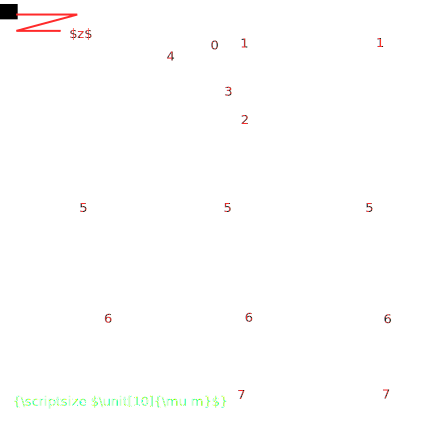
\includegraphics[width=8cm]{m_wf}
    \svginput{.6}{m_wf}
    \svginput{.6}{m_sec}
    \caption{{\bf left:} Wide field focus series of a
      three-dimensional distribution of yellow-green beads in agarose
      gel. Sampling in $z$ is $\unit[1]{\mu m}$. {\bf left:}
      Computationally sectioned images of the same sample. The
      corresponding raw images are shown in \figref{fig:m_phase}.}
  \label{fig:m_wf}
\end{figure}

\begin{figure}[htbp]
  \centering
  %
\includegraphics[height=.6\textheight]{m_phase}
  \svginput{1}{m_phase}
  \caption{Focal stack with structured illumination of the same sample
    as \figref{fig:m_wf}. For each $z-$slice (rows) four exposures with
    different grating phase (columns) were acquired.}
  \label{fig:m_phase}
\end{figure}


In those cases \cma{optical sectioning} it is useful to utilize
structured illumination to separate out-of-focus and in-focus
fluorescence. The mosaic on the right of \figref{fig:m_wf} shows the
computed optical sections from four raw images per slice. The raw
images are displayed in \figref{fig:m_phase}.  The optical sections
contain relatively distinct vertical reconstruction artifacts. These
can be avoided by using the HiLo reconstruction method which has the
additional advantage of only needing two raw images per slice.

However, \cma{bead localization} the HiLo method needs considerably
more programming. Also, the artifacts have no effect on the localization
precision of the algorithm. For localization, I determine the center of
each bead by finding local maxima after applying a three-dimensional
difference of Gaussian filter (matched to the bead diameter). The
resulting coordinates are depicted in the inlay in \figref{fig:m_ang}.

% \begin{figure}[hbtp]
%   \centering
%   \svginput{.7}{m_sec}
%   \caption{}
%   \label{fig:m_sec}
% \end{figure}

In the next step, each bead is illuminated individually by displaying
a bright disk at the corresponding position on the focal plane SLM,
while the pupil plane SLM displays a mask which prevents
exposure of out-of-focus beads. This mask is calculated automatically
with a raytracer and utilizes the three-dimensional model of the bead
distribution.


\begin{figure}[hbtp]
  \centering
  \svginput{1}{angular-beads}
  \caption{{\bf left inlay:} Coordinates of the beads from
    \figref{fig:m_wf}. {\bf top mosaic:} Camera images with
    spatio-angular illumination of the beads. This is not a focus
    series but an image of each individual bead. {\bf bottom mosaic:}
    Corresponding patterns of the pupil plane SLM.}
  \label{fig:m_ang}
\end{figure}

The eight camera images of the individual beads are shown in the two
top rows in \figref{fig:m_ang}. Unlike \figref{fig:m_wf}, no focal
series is shown. Each image is focused on a single bead. The
corresponding pupil plane SLM masks are shown in the two rows below. I
will briefly describe \cma{description of pupil plane masks} the
construction of the masks using bead 4 as an example. According to the
three-dimensional diagram in the inlay in \figref{fig:m_ang}, bead 4 is
on the edge of the bead distribution. The smallest angle relative to
the optical axis is between the connecting line of bead 4 and
7. Therefore, the single ``shadow'' (indicated with an arrow) in the
pupil plane mask corresponds to bead 7. All other beads would only be
illuminated by light that strikes bead 4 under a larger angle. Bead 6
and maybe bead 5 combine to the second shadow on the periphery of the
pupil.

The \cma{stability} camera images of bead 2 and 7 in
\figref{fig:m_ang} stand out because they are completely dark. The
reason is that the registration between the focal plane SLM and camera
has shifted by a few microns between localizing the beads and their
spatio-angular exposure. This type of error was corrected by removing
rubber feet from the microscope and screwing it directly to the metal
table.

 

A \cma{artifacts} more interesting effect is visible in the camera
image of bead 5. Only the bottom half of the bead is illuminated but
due to fluorescence in the agarose gel, the circular area that is
illuminated by the focal plane SLM is still visible. This effect would
predominantly occur in samples where fluorescent areas are not sharply
defined. As exposures with light from different angles will contain
different contributions of background fluorescence, it is not clear
whether individual sub-images of the spatio-angular microscope can be
joined into a seamless image. The image quality of confocal
microscopes hardly seems achievable by our system. Cells in an embryo can probably
be counted and tracked, but a quantitative measurement of the
fluorescence seems difficult.

I \cma{comparison spatial control and only angular control} imaged the
beads in \figref{fig:m_ang} with both full angles and optimized
angles. The selective illumination of individual beads using
only the focal plane SLM and full angles already reduced the background
fluorescence from other beads and the gel
significantly. Unfortunately, it is not possible to discern any
further improvement with additional angular control.  I think the
fluorescence from out-of-focus beads can not be detected in the presence of photon
shot noise of the fluorescence from the gel. Angular control will
still have a positive effect because out-of-focus beads are not
uselessly exposed --- it is just not possible to measure this in this
particular sample.

\section{Angular illumination and a higher concentration of beads}
In order to measure the influence of angular illumination control
directly, I made another sample with higher concentration of beads in
an agarose gel with significantly less fluorescence.


\begin{figure}[!hbt]
  \centering
  \svginput{.9}{montage-ang}
  \caption{Dense beads in agarose gel {\bf top left:} Wide field image
    of the beads. The target bead is highlighted with a white circle.
    {\bf bottom left:} Target bead is selectively illuminated by the
    focal plane SLM (using all angles).  {\bf right mosaic:} Variation
    of illumination angle. The contrast of out-of-focus beads is
    increased by scaling the values with a factor of 100 compared to
    the two images on the left.}
  \label{fig:montage-ang}
\end{figure}

The images are shown in \figref{fig:montage-ang}. In the wide field
image, I indicate one bead with a white circle. In the other images,
this bead is selectively illuminated using the focal plane SLM white
circle with dashed outline.

For simplicity, I have omitted the raytrace illumination optimization
and just vary a circular window on the pupil plane SLM ($\rho=0.7,
r=0.3$, with the same geometry as in \figref{fig:overview-bleach}~(e)).


In the mosaic on the right side of \figref{fig:montage-ang}, the
intensity is displayed with a factor of $100\times$ compared to the
previous two images. The same scaling is applied to the images of the
mosaic. The intensity of the central bead is clipped. The illumination
cone that moves with the window manifests itself as a change in the
relative intensities of the out-of-focus beads. A difference can be
seen, for example, in the point marked by an arrow in the pictures for
$\theta=30^\circ$ and $\theta=330^\circ$.

\section{Conclusion}
The described experiments demonstrate that the hardware of the
microscope is functioning as intended, although the performance is
impaired by low transmission and long pattern loading times.

Especially for the experiment in section \ref{sec:beads_under}, a lot
of software had to work in conjunction. The mapping between focal
plane SLM and camera has to be established, the beads must be located
and optimal illumination patterns must be found. These algorithms
should work in close combination with the hardware control, so that
the entire experiment can run with as little user interaction as
possible and finish within reasonable time.

% Das Hauptproblem und der groesste Zeitaufwand lag hier vor allem an
% nicht ausreichenden Informationen ueber einige der nicht ersetzbaren,
% alternativlosen Hardwarekomponenten.

%%% Local Variables: 
%%% mode: latex
%%% TeX-master: "kielhorn_memi"
%%% eval: (reftex-mode)
%%% eval: (flyspell-mode)
%%% End: 

\chapter{Discussion}
\label{sec:discussion}
This thesis deals with the practical development of a wide-field
fluorescence microscope system that can control the irradiance in the
specimen as well as the illumination angles with the aim of decreasing
phototoxicity.

The original \cma{origin of the idea} idea was to combine a
programmable array microscope with a control of the illumination
directions. Initially this seems to be an elegant approach: The
programmable array microscope produces two images on a camera, one of
which contains only out-of-focus light. By variation of the
illumination angle of the excitation light, it should be possible to
find the direction with minimal out-of-focus contributions.
 
Fairly quickly it became clear that this approach, if at all, would
work only inefficiently. After all, for the programmable array
microscope to work, fine structures must be imaged into the
specimen. This, however, has the consequence that several diffraction
orders instead of one bundle of rays with similar directions must
traverse the sample. For most specimens this will bring no advantage
compared to a wide-field microscope.

We opted instead for a modification of the excitation path in a
wide-field microscope. My assumption was that given an estimate of the
'to-be-imaged' three-dimensional fluorophore distribution, and perhaps
additional information on the expected movement of cells, pathogens or
organs; a sufficiently accurate prediction of the expected
out-of-focus light can be made.

Using \cma{description of the hardware} two spatial light modulators
(SLM), we can project appropriate distributions of excitation light
into the sample. One SLM controls the angle and the other the in-focus
pattern of light. Our goal for the instrument was that it can capture
one stack per minute, consisting of twenty slices. For this, partial
recordings of slices should be acquired in sequence and later composed
into one image. Therefore We selected the SLM devices with an emphasis
on high speed.

The fastest commercially available SLM are ferroelectric liquid
crystal on silicon devices (fLCoS) and digital micro-mirror devices
(DMD), which both can only do binary modulation. However, in our case
binary intensity modulation is disadvantageous. Sharp edges lead to
high diffraction losses and strong oscillations of the field in the
Fraunhofer diffraction pattern.

The pupil \cma{Why Fraunhofer micro-mirror array?} plane SLM, that
controls the illumination angles does not necessarily need a high
resolution but a binary SLM device should be avoided here because
otherwise oscillations of excitation intensity would occur in the
specimen and appear on the camera image. For this reason, we use a
specifically developed SLM, which resembles a DMD in terms of mode of
operation and speed but can display gray scale values.

The focal plane SLM, on the other hand, should have a high resolution
\cma{choice for focal plane SLM} and it should be possible to update
its patterns very fast, depending on recent camera
acquisitions. Initially I opted for a SLM that is connected to the
graphics card of a computer. We chose a fLCoS SLM because its pixel
borders are less sharp than the DMD and we expected a better
efficiency for our application. Unfortunately there were difficulties
with the synchronization of the graphics card and the other
devices. Therefore, relatively late into the project I had to replace
the SLM controller with another one that contains internal memory and
is linked to a computer via USB.  \nomenclature{USB}{Universal Serial
  Bus.} Unfortunately, the USB connection is very slow and fast update
of image patterns is no longer possible. In retrospect, it would have
been easier to use two identical gray value SLM from Fraunhofer. Note
that Institut Pasteur and Fraunhofer IPMS continue this work and do
just that under the Joint-Programme Inter Carnot Fraunhofer PICF 2011,
``Micromirror Enhanced Microscopic Imaging for high-speed angular and
spatial light control in spectral Optogenetics and Photomanipulation
applications in biological applications'' (MEMI-OP).

A \cma{remedy against low acceptance angle} serious disadvantage of
the Fraunhofer SLM in combination with the Fourier optical filter
approach employed in our prototype is the small acceptance angle. This
limits the exposed field to $\unit[80]{\mu m}$ diameter for a
wavelength of \unit[473]{nm} using a $63\times$ objective with a
numerical aperture of $1.4$, while the objective does support
$\unit[400]{\mu m}$ field diameter. One solution could be contrast
generation in a common path interferometer as described in the patent
application \citep{Heintzmann2010a}. The approach is derived from
reflective Nomarski differential interference contrast microscopy. A
birefringent prism separates the illumination bundle into bundles that
have a small offset (shear).  If the shear distance corresponds to the
pixel pitch $\Lambda=\unit[16]{\mu m}$ of the micro-mirrors then this
device converts height differences between adjacent mirrors into
intensity contrast. My experiments with a set of Nomarski prisms that
were available in our lab gave an indication, that this method can
work. However the prisms had too small a shear angle and returning
diffraction orders were cut off. At this point in time, the planning
for the original prototype was already so far advanced that a change
was not possible. However, this is still a very promising method and
will probably produce good results when prisms with larger shear
angles are used. Additionally it should be noted that this method will
work better for piston-type micro-mirrors than for torsion
micro-mirrors.

Given \cma{priority of the control algorithm} the \emph{low
  transmission} of our prototype, which could be just barely enough to
investigate the biological test system of \celegans\ embryos, the
disproportionally high effort that went into synchronizing the two
fast SLM which can only run at a \emph{reduced duty cycle}, and the
\emph{limited etendue} which excludes some interesting experiments, it
would have been better in hindsight, to build a demonstrator with two
slow, conventional, gray-value SLM and to spend more effort on the
development of the illumination control algorithm.

In \cma{holographic system} this context, with the aim of simplifying
the hardware, I built a holographic illumination system consisting of
a single phase-only SLM in the intermediate image plane. This enables
simultaneous control of both, the in-focus light distribution as well
as the illumination angles in the specimen. The SLM displays
diffraction gratings and its arrangement is such, that the first
diffraction order illuminates the pupil. The illumination angle in the
specimen can be adjusted by the grating period and direction while the
local irradiance is controlled with the grating contrast.


  % - holographie loest jedoch nicht das problem geringer ettendue (die moegliche
  %   ettendue muss ich mir genauer ueberlegen, sie haengt mit der
  %   anzahl der pixel des displays und den grating konstanten zusammen,
  %   die dargestellt werden koennen, da das system off-axis betrieben
  %   werden muss, wird die ettendue geviertelt)

Unfortunately the phase-only SLM that I used for the experiments
suffers from cross-talk between pixels, a non-linear transfer function
and temporal fluctuations of the displayed phase pattern. It was
uncertain whether these problems could be circumvented. Especially
higher orders which are generated by the device's non-linearity and
that can reach the sample are a problem, and it seems particularly
difficult to project a finely structured grid into the sample.
Projecting such patterns is necessary, because for my illumination
algorithm I need a reasonably good measurement of the
three-dimensional fluorophore distribution. For many specimen
structured illumination is necessary to remove out-of-focus light from
the raw images and obtain optical sections.  Phase SLM which became
available more recently have a much better performance and could
probably be used to construct a holographic spatio-angular
illumination device.

Our \cma{sectioning by structured illumination} prototype with two SLM
is more suitable for structured illumination. The period on the focal
plane SLM and the illumination aperture defined by the pupil plane SLM
can be selected for best possible contrast of the in-focus light
pattern. Optically sectioned images can the be calculated with the
usual methods. The HiLo method proposed by Jerome Mertz and best
documented in \cite{Mertz2010} is preferable to others as only two
exposures per slice are necessary. Since images in our system are
taken in rapid succession and movement artifacts are unlikely, we
developed a variant of the HiLo method and in contrast to the
original, which uses one uniformly illuminated image and one with
structured illumination, we use two structured illumination images
which gives better signal-to-noise.

During my work on the project \cma{sCMOS --- new camera technology} a
much improved camera technology came to market. No such camera was
used for measurements in this work, however, such a camera could be
added to our system without substantial changes. 

This change is made \cma{Arduino for control electronics} possible
mostly due to the flexibility that the Arduino gives. This cheap and
easy to use electronics platform has been used for several years in
our lab and is particularly useful for synchronization of multiple
devices. The source code for the Arduino microcontroller is often
short and relatively easy to read. This controller is thus well suited
to document the logic in our synchronization circuits and can be
easily understood and extended by new members of our group.

During this work, I used many different electronic devices (SLM:
Hamamatsu, Holoeye, ForthDD, Texas Instruments, Fraunhofer, cameras:
Andor (Clara, IXon2, IXon3, IXon Ultra, Neo sCMOS), Photometrics
Cascade II, Hamamatsu (Orca Flash 2.8 and 4.0), Logitech Pro 9000, and
more). I noticed that construction and debugging effort depend very
much on the quality of the documentation. If documentation is
insufficient, which unfortunately is often the case, then it helps if
communication is done with open standards (USB video device class,
Ethernet).

Particularly positive I was surprised by the Texas Instruments
DMD. The SLM development kit is very mature \citep{Guide2012},
contains open source software and high quality documentation
explaining even the control registers of individual chips. While
working with the kit I was able to implement features within three
days, for which I spent several months of reverse engineering and
trial and error on devices of other manufacturers --- most notably,
the fastest possible image update with 1440 frames per second via
HDMI. If I had known that before, I would have designed the prototype
differently and I would have accepted some drawback regarding optical
performance.

I \cma{Open hardware is a good thing} am particular unhappy with the
state of scientific cameras as all of them gave me problems with
incompatible or unstable drivers. Therefore, I hope that there will be
more projects that open their resources to the public, such as Marc
Levoy's Franken Camera \citep{Adams2010}; or that the manufacturers of
the ever-improving consumer cameras document and disclose the
protocols for disabling automatic image processing and accessing raw
sensor data for their devices (as with the Logitech Pro 9000).


%Fu2011

Our \cma{results of existing control software} prototype and the
software for illumination optimization has been designed for the
observation of cells in a developing \celegans\ embryo. So far I was
able to demonstrate spatio-angular illumination on static, non-living
samples. So far I have not applied the method for living
organisms. Here, the main problem is that image upload, especially to
the focal plane SLM takes disproportionally long.

\section{Outlook}

If \cma{proposal of an optogenetics experiment} the sample does not
change very fast, and plenty of time is available to upload images
into the SLM controllers, then the current prototype allows
experiments with rapidly changing illumination patterns (about 1000
fps should be possible). One interesting biological experiment would
be similar to \cite{Branco2010}. There, synapses were excited by
moving a focal spot along one linear dendrite and its response was
recorded as a function of the speed of the focal spot. With our
system, two branches of a dendrite could be stimulated simultaneously
and the response of the junction could be investigated.

The \cma{next steps for control software} algorithm for the
optimization of the illumination patterns can still be improved. So
far, I assume that the sample can be represented well by spheres. The
nuclei in each slice are illuminated individually and the algorithm
finds illumination angles so that exposure of out-of-focus nuclei is
avoided. An obvious improvement would be to find nuclei that can be
illuminated with similar angles and group them for simultaneous
exposure. Even better would be an algorithm that does not need to
represent the specimen as solid bodies but works directly on stacks of
optical sections. In a first simple experiment, using the graphics
processing unit, I could show that the extensive calculations can be
carried out in reasonable time frames.


Our work \cma{partial coherent simulation} also leaves an unanswered
question regarding the optics. It would be interesting to simulate the
wave-optical image formation of the prototype with partial
coherence. This would answer the question how important the gray
levels of the micro-mirror array in the pupil-plane really are, and
whether or not we can replace it with a binary DMD.

A similar simulation should be used to investigate the influence of
field mask B0 and Fourier stop B1 on the contrast and the transfer
function of the schlierenoptics system.




% - eine genaue analyse einiger probleme mit wellenoptischer partiell
%   kohaerenter theorie steht noch aus und waere interessant (nach
%   wichtigkeit)

%   - partiell kohaerente simulation des mma im schlierenoptischen system

%     - sind graulevel vorteilhaft?

%     - wuerde ein mma, bei dem alle spiegel in dieselbe richtung kippen
%       die ettendue verdoppeln?

%   - partiell kohaerente simulation des mma im shearing
%     interferometrischen system

%     - was ist die maximale ettendue eines wollaston prismas?

%   - holographie methode mit extended source

  % - Denkbar waere auch ein scannendes konfokales Mikroskop, dass an
  %   die Beleuchtungswinkel an jedem Punkt kontrolliert (siehe
  %   fig:hourglass-all-b).  Bisher wurden in der Literatur nur Systeme
  %   beschrieben, die die Phase des Beleuchtungslicht in der Pupille
  %   aendern (FIXME ref). Eine Adaption dieser Systeme zu einem
  %   spatio-angularen ist naheliegend und ich schlage vor, derartige
  %   Systeme auch untersucht werden sollten. Die Kombination von CLEM,
  %   einem Ringdetektor (vielleicht mit UZI) koennte die Bildgebung im
  %   Inneren lebender Organe (z.B. Gehirn) verbessern.

\appendix
\chapter{EM-CCD camera calibration}
\section{Andor Basic code listing for automatic image acquisition}
\label{sec:basic-acquisition}
\definecolor{light-gray}{gray}{0.95}

\lstdefinestyle{myframe}{
  basicstyle=\LSTfont,
  % basicstyle=\footnotesize\ttfamily,
  rulesepcolor=\color{gray} ,
  rulecolor = \color{black},
  frame = single,
  % framerule = 0pt,
 % backgroundcolor =\color{light-gray}, 
  fontadjust=true,
  breaklines = true,
  showstringspaces=false,
  commentstyle=\itshape,
}
\lstdefinestyle{mymaxima}{
  language=C,
  title={Maxima},
  style=myframe
}
\lstdefinestyle{myclang}{
  language=C,
  title={C language},
  style=myframe
}
\lstdefinestyle{myfortran}{
  language=Fortran,
  style=myframe
}
\lstdefinestyle{mymatlab}{
  language=Matlab,
  title={Matlab},
  style=myframe
}
\lstdefinestyle{mylisp}{
  language=Lisp,
  title={Common Lisp},
  style=myframe
}
\lstdefinestyle{mybasic}{
  title={Andor Basic},
  language=[Visual]Basic,
  style=myframe
}
\lstdefinestyle{mypython}{
  language=Python,
  title={Python},
  showstringspaces=false,
  tabsize=4,
  basicstyle=\ttfamily,
  morekeywords={models, lambda, forms},
  frame = single,
  breaklines = true,
  style=myframe
}

The following code allows to record data for calibration of a Andor
EM-CCD with as little user interaction as possible. More detail is
given in the main text in section \ref{sec:ccd-intro} on page
\pageref{sec:ccd-intro}.

The program is written in a dialect of Basic and automates the Andor Solis software.
Before use, a picture resembling
\figref{fig:shot-noise} on page \pageref{fig:shot-noise} should be
imaged onto the sensor, e.g.\ a defocused fluorescent sample. The
acquired data can later be processed using either the Matlab/DIPimage
function \verb!cal_readnoise! or, equivalently, by using the Python
script from the next section.

A camera calibration allows to convert image data into the device
independent unit of effective photoelectrons but this only works as
long as data acquisition occurs at the same camera settings (pre-amp
gain, EM-gain, sensor temperature, vertical shift speed, readout rate,
...) as those that were used for the calibration. This Basic program
measures data for a wide range of EM-CCD amplification settings, but
it could easily be adopted to analyze other parameters as well.

The camera that I have used in the development of this program
comprises an internal mechanical shutter. This is useful because it is
important that for each parameter setting at least one dark image is
acquired (but it is better to acquire two dark images and use the
second). Ultimately, dark images are necessary to quantify the readout
noise.

The code listings in this section are supposed to be in this sequence
in a single source file.

For this program I assume that the camera is illuminated with a
continuous flux of photons. The program is designed to acquire images
with a wide range of EM gains. Since the photon flux remains constant
but amplification varies greatly, I acquire one image with a short
$\unit[10]{\mu s}$ exposure prior to each measurement. The following
function searches for the maximum value in this image and calculates
an appropriate exposure time so that a maximum of \unit[10000]{ADU}
will be obtained in the preceeding acquisitions.
\begin{lstlisting}[style=mybasic]
function ~GetSaturatingExposure()
        SetKineticNumber(1)
        exp=.01
        SetExposureTime(exp)
        run()
        m=maximum(#0,1,512)
        GetSaturatingExposure=exp*10000/(m-100) % 100 is the background in ADU
        CloseWindow(#0)
return
\end{lstlisting}
The following code listing selects the conventional readout register
of the sensor (a register without EM multiplication), acquires 20
images without and then with light by calling the function
\verb!run()! and stores the data in a TIF image file.
\begin{lstlisting}[style=mybasic]
name$ = "C:\Users\work\Desktop\martin\20111111\scan-em3\ixon_"
print("start")

SetOutputAmp(1)
print("conv_start")
exp= ~GetSaturatingExposure()
print(exp)
SetExposureTime(exp)
SetKineticNumber(20)
SetShutter(0,1)
run()
save(#0,name$ + "conv1_dark.sif")
ExportTiff(#0, name$ + "conv1_dark.tif", 1, 1, 0, 0)
CloseWindow(#0)
CloseWindow(#1)

SetShutter(1,1)
run()
save(#0,name$ + "conv1_bright.sif")
ExportTiff(#0, name$ + "conv1_bright.tif", 1, 1, 0, 0)
CloseWindow(#0)
CloseWindow(#1)
\end{lstlisting}
\comment{ $ } The loop in the next listing makes similar acquisitions
for a range of EM gains.  Evaluating the data revealed that a settling
time of a few seconds should be allowed for after calling
\verb!SetGain!. After all, there are relatively high voltages. I
inserted a comment in the corresponding line.
\begin{lstlisting}[style=mybasic]
SetOutputAmp(0)
SetShutter(1,1)
for i = 40 to 300 step 10
        SetGain(i)
        % here should be a 3s wait
        exp=~GetSaturatingExposure()
        print(exp)
        SetExposureTime(exp)
        SetKineticNumber(20)
        SetShutter(0,1)
        run()
        save(#0,name$ + str$(i) + "_dark.sif")
        ExportTiff(#0, name$ + str$(i) + "_dark.tif", 1, 1, 0, 0)
        CloseWindow(#0)
        CloseWindow(#1)
        SetShutter(1,1)
        run()
        save(#0,name$ + str$(i) + "_bright.sif")
        ExportTiff(#0, name$ + str$(i) + "_bright.tif", 1, 1, 0, 0)
        CloseWindow(#0)
        CloseWindow(#1)
next
\end{lstlisting}
Finally I acquire a last measurement with the conventional readout
register: \begin{lstlisting}[style=mybasic]
SetOutputAmp(1)
print("conv_end")
exp= ~GetSaturatingExposure()
print(exp)
SetExposureTime(exp)
SetKineticNumber(20)
SetShutter(0,1)
run()
save(#0,name$ + "conv2_dark.sif")
ExportTiff(#0, name$ + "conv2_dark.tif", 1, 1, 0, 0)
CloseWindow(#0)
CloseWindow(#1)
        
SetShutter(1,1)
run()
save(#0,name$ + "conv2_bright.sif")
ExportTiff(#0, name$ + "conv2 _bright.tif", 1, 1, 0, 0)
CloseWindow(#0)
CloseWindow(#1)
\end{lstlisting}
Table \ref{tab:ixon-table} summarizes results of calibration
measurements that were acquired using this software and evaluated
using the Python code from the next section.

Unfortunately, the data in the first and last line (conv1 and conv2
with $M=1$) show a disparity in the pre-amplifier gain
$M_\textrm{pre}$. An improvement would be to use an LED light source
(which doesn't bleach) or intersperse conventional readouts between
measurements with EM gain in order to compensate for variations due to
bleaching.

% 1.3165/1.593*15496 = 12806 < 14923

\begin{table}[!htbp]
  \centering
%  \begin{tabular}{|l|l|l|l|l|l|l|l|}
  \begin{tabular}{r l l r  l r l}
\toprule
$\textsf{gain}_\textrm{software}$ & $1/(M\cdot M_\textrm{pre})$ & $N_r$ & $N_{(M)}/(W\times H)$ &  \textsf{exposure} & $N_{(M)}'/(W\times H)$ & $1/F_n$ \\
 & [$e^-/$ADU] & [$e^-/$px] & [$e^-/$px] & [ADU] & [s] & [$e^-/$(px s)]  \\
\midrule
conv1 & 1.3165 & 7.189 & 3008.66      & 0.2016 & 14923 & 0.981 \\
50 & 0.1160 & 0.486 & 260.05 & 0.0289 & 8995 & 0.591 \\
60 & 0.0984 & 0.406 & 225.46 & 0.0249 & 9054 & 0.595 \\
70 & 0.0841 & 0.349 & 190.52 & 0.0212 & 8983 & 0.591 \\
80 & 0.0729 & 0.305 & 165.24 & 0.0186 & 8907 & 0.586 \\
90 & 0.0680 & 0.288 & 150.54 & 0.0161 & 9368 & 0.616 \\
100 & 0.0611 & 0.262 & 128.47 & 0.0136 & 9427 & 0.620 \\
110 & 0.0550 & 0.241 & 121.11 & 0.0129 & 9409 & 0.619 \\
120 & 0.0510 & 0.228 & 113.71 & 0.0120 & 9498 & 0.624 \\
130 & 0.0465 & 0.211 & 106.66 & 0.0112 & 9541 & 0.627 \\
140 & 0.0433 & 0.201 & 96.95 & 0.0101 & 9564 & 0.629 \\
150 & 0.0405 & 0.192 & 89.68 & 0.0093 & 9671 & 0.636 \\
160 & 0.0380 & 0.183 & 87.24 & 0.0090 & 9656 & 0.635 \\
170 & 0.0359 & 0.175 & 81.56 & 0.0084 & 9739 & 0.640 \\
180 & 0.0339 & 0.169 & 79.80 & 0.0081 & 9863 & 0.648 \\
190 & 0.0321 & 0.163 & 74.00 & 0.0075 & 9806 & 0.645 \\
200 & 0.0305 & 0.158 & 72.57 & 0.0073 & 9878 & 0.649 \\
210 & 0.0292 & 0.155 & 69.44 & 0.0070 & 9944 & 0.654 \\
220 & 0.0280 & 0.150 & 67.69 & 0.0068 & 9971 & 0.656 \\
230 & 0.0268 & 0.147 & 65.63 & 0.0065 & 10057 & 0.661 \\
240 & 0.0257 & 0.188 & 63.90 & 0.0063 & 10131 & 0.666 \\
250 & 0.0244 & 0.140 & 62.52 & 0.0062 & 10026 & 0.659 \\
260 & 0.0237 & 0.137 & 62.86 & 0.0062 & 10078 & 0.663 \\
270 & 0.0229 & 0.135 & 63.17 & 0.0062 & 10130 & 0.666 \\
280 & 0.0221 & 0.133 & 63.64 & 0.0062 & 10204 & 0.671 \\
290 & 0.0214 & 0.130 & 63.38 & 0.0062 & 10162 & 0.668 \\
300 & 0.0205 & 0.128 & 63.20 & 0.0062 & 10133 & 0.666 \\
conv2 & 1.5953 & 8.768 & 8198.86 & 0.5291 & 15496 & 1.019 \\
\bottomrule
\end{tabular}
%  \includegraphics[width=12cm]{../app_cam/ixon3}
\caption{Comparison of read noise for different EM-gain settings
  (first column) of the Andor IXon3. $W$ and $H$ are the size of the sensor (in pixels). The value $N_{(M)}'$
  estimates the number of photoelectrons the detector would have
  seen with \unit[1]{s} integration time and is used to calculate
  the excess noise factor in the last column. In EM-mode the fastest
  readout speed was used (\unit[10]{MHz}) with the default vertical shift speed of
  \unit[1.7]{$\mu$s}.}
  \label{tab:ixon-table}
\end{table}

\newpage

\section{Python code listing for the read noise evaluation}
\label{sec:python-readnoise-eval}
Here I present a Python implementation for evaluating data that has
been recorded using the program from the previous
section. \figref{fig:ixon} shows two evaluations for data with and
without EM-gain using an Andor IXon3 EM-CCD camera.

\begin{figure}[htbp]
  \centering
  \pdfinput{17cm}{ixon_conv1}
  \pdfinput{17cm}{ixon_300}
  \caption{Readout noise evaluation using the Python code {\bf top:}
    Conventional readout of an Andor iXon3 camera. {\bf bottom:}
    readout with an EM-gain setting of 300 on the same camera with
    identical sample. {\bf left:} 2D histogram of per pixel variances
    against binned intensities. red data points: measuremnts, blue
    line: linear fit {\bf middle:} variance of 20 dark images. {\bf
      right:} mean of 20 dark images.}
  \label{fig:ixon}
\end{figure}
The following code loads several Python packages. Essentially, I use
\verb!numpy! by loading \verb!pylab! \citep{Jones} for the data
analysis tasks and the package \verb!matplotlib! \citep{Hunter:2007}
for visualizing the results.
\begin{lstlisting}[style=mypython]
#!/usr/bin/env python
# usage:   ti.py DIRECTORY CAMERA_NAME EM_GAIN
# example: ti.py /media/backup/andor-ultra-ixon/martin/20111111/scan-em3/ ultra 2700
import sys
import os
import matplotlib
matplotlib.use('Agg')
from pylab import *
from libtiff import TIFFfile, TIFFimage
from scipy import stats
seterr(divide='ignore')
\end{lstlisting}
When starting the program I specify which data should be loaded using
command line parameters. The following code will read in the measured
image data with and without illumination.
\begin{lstlisting}[style=mypython]
folder = sys.argv[1]
cam = sys.argv[2]
gain = sys.argv[3]

def readpics(gain,cam='ixon_',isdark=False):
    print 'loading ', os.path.join(folder,cam) + '_' + gain + '_bright.tif'
    fg=TIFFfile(os.path.join(folder,cam) + '_' + gain + '_bright.tif')
    bright,bright_names=fg.get_samples()
    bg=TIFFfile(os.path.join(folder,cam) + '_' + gain + '_dark.tif')    
    dark,dark_names=bg.get_samples()
    return (bright[0],dark[0])

(f,b) = readpics(gain=gain,cam=cam)
\end{lstlisting}
The next code listing creates a two-dimensional histogram with 64 bins
for variances and 128 bins for intensities.
\begin{lstlisting}[style=mypython]
ny,nx=64,128
H,y,x=histogram2d(v.flatten(),i.flatten(),bins=[ny,nx],
                  range=[[0,v.max()],[0,i.max()]])
extent = [x[0], x[-1], y[0], y[-1]] 

fig=figure(figsize=(24, 8),dpi=300)
hold(False)
title('bal')
subplot(1,3,1)
imshow(log(H), extent=extent,
           aspect='auto', interpolation='none',origin='lower')
hold(True)
\end{lstlisting}
The histogram is not strictly necessary for the analysis but gives an
overview of the measured data at a quick glance, i.e.\ if there were
enough measurements for all intensities and whether the sensor was
over-exposed.

The most important part of the evaluation is performed in the
following code segment. Here I accumulate data in the variables
\verb!acc! and \verb!accn! that is later used to determine the average
values of the variances for all intensities.
\begin{lstlisting}[style=mypython]
acc=zeros(x.shape,dtype=float64)
accn=zeros(x.shape,dtype=int64)
s=nx/i.max()
for ii,vv in nditer([i,v]):
    p=round(ii*s)
    acc[p]+=vv
    accn[p]+=1   
\end{lstlisting}
Subsequently, I determine the parameters for a linear fit of the
variances vs.\ intensities, utilizing only the first 60\% of the
intensities so that any non-linearities that might occur at higher
intensities do not affect the slope.
\begin{lstlisting}[style=mypython]
ax=x[nonzero(accn)]
ay=acc/accn
ay=ay[nonzero(accn)]
l=round(.6*len(ax))
bx=ax[0:l]
by=ay[0:l]
plot(ax,ay,'r+')
slope,intercept,rval,pval,stderr=stats.linregress(bx,by)
\end{lstlisting}
From the slope of the line I determine the conversion factor to change
the ADU units into the device-independent unit of photoelectrons. With
this I convert the variance of the dark images into readout noise in
terms of photoelectrons per pixel.
\begin{lstlisting}[style=mypython]
plot(ax,polyval([slope,intercept],ax))
xlabel('intensity/ADU')
ylabel(r'variance/ADU$^2$')
real_gain=1/slope # unit electrons/ADU
read_noise=sqrt(var(b))*real_gain # electrons RMS per pixel
mean_elecs=(mean(f)-mean(b))*real_gain # photoelectrons electrons per pixel
print gain,cam,real_gain,read_noise,mean_elecs,mean(b),rval,pval,stderr
tit='EM-gain: %s, cam: %s, real gain: %.2f e/ADU\n
read noise: %.2f e RMS/pixel, mean: %.2f e/pixel, offset: %.2f'
% (gain,cam,real_gain,read_noise,mean_elecs,mean(b))
title(tit)
subplot(1,3,2)
imshow(var(b,axis=0))
title('variance of darkimages')
colorbar()
subplot(1,3,3)
imshow(mean(b,axis=0))
title('mean of darkimages')
colorbar()
show()
fig.savefig(cam+'_'+gain+'.png')
\end{lstlisting}


\chapter{Optical sectioning by structured illumination using the HiLo method}
\label{sec:sectioning}
\begin{summary}
  In this chapter I compare three methods to calculate optical
  sections from fluorescence microscope images with structured
  illumination. I employ the wave-optical model of image formation
  (see section \ref{sec:wave-image-formation}) to simulate focal
  stacks with structured illumination of a three-dimensional
  fluorophore distribution. 

  The code in this chapter permits to simulate aberration-free imaging
  and to compare the performance of sectioning algorithms at different
  light levels, i.e.\ in the presence of photon shot noise.
\end{summary}

\comment{
\jpginput{}{m_phase}{}
}

First, I will construct a three-dimensional fluorophore
distribution. Then I will calculate the three-dimensional point spread
function $h(\r)$ of a high-aperture immersion objective with
$\textrm{NA}=1.4$ and $n=1.52$ using equations (\ref{eq:psf}) and
(\ref{eq:asf}) on page \pageref{eq:asf}. Using this three-dimensional
array (denoted by \verb!psf(:,:,:)! in the code), the
three-dimensional light distribution in the sample, as well as images
on the camera can be calculated by a convolution operation.

For the numerical simulation I use the DIPimage Toolbox for Matlab
\citep{dipimage} as it permits to express the required image
processing algorithms with a relatively elegant syntax.

The \cma{syntax of DIPimage} following code listing fills a
three-dimensional array with the geometric primitives line, rectangle
and a sphere shell. The function \verb!newim(GX,GX,GX)! creates a new
DIPimage data object. In general, DIPimage functions can receive their
arguments either explicitly, as in this case, or implicitly by calling
with another DIPimage data object, e.g.\ when calling \verb!rr(g2)!
when constructing the hollow sphere. This function returns an array
where each element contains the distance to the central pixel. The
comparison operation results in a Boolean data type which I implicitly
turn back into a floating point number by adding a zero.

To save computing time when applying the section algorithms, I cut
\verb!S! to the smallest dimensions, so that it still contains the
complete object.  The figure next to the code shows the geometry of
the three-dimensional fluorophore distribution and three small images
on the right are simulated widefield images of the planar objects.

\begin{lstlisting}[style=mymatlab]
global GX; GX = 64; g2 = newim(GX,GX,GX); % make empty 3d image
line_z=floor(size(g2,3)/2)-3;
lineseg = drawline(g2,floor([.3*GX 0 line_z]),floor([.8*GX .9*GX line_z]),1);

rect_x0 = floor(.2*GX); rect_x1 = floor(.9*GX);
rect_y0 = floor(.2*GX); rect_y1 = floor(.5*GX);
rect_z1 = floor(GX/2)+3;
rectangle1 = newim(g2);
rectangle1(rect_x0:rect_x1,rect_y0:rect_y1,rect_z1)=1;

rect_x0 = floor(.6*GX); rect_x1 = floor(.8*GX);
rect_y0 = floor(.0*GX); rect_y1 = floor(.9*GX);
rect_z2 = floor(GX/2)+9;
rectangle2 = newim(g2);
rectangle2(rect_x0:rect_x1,rect_y0:rect_y1,rect_z2)=1;

hollow_sphere = 0.0 + (.3<rr(g2,'freq') & rr(g2,'freq')<.4); 

S = 12 * lineseg + 4 * (rectangle1 +rectangle2) + hollow_sphere;
[unused1,unused2,S] = bbox(S>0,S); clear g2;
\end{lstlisting}  %3.33cm hoch
\vspace{-6.33cm}\hspace{9cm}
\svginput{1}{hilo-sec-S}

\vspace{3cm}

Mit dem folgenden Code berechne ich zunaechst die
generalisiert McCutchen Apertur a fuer ein Objektiv mit gegebener
numerischer Apertur. Dafuer berechne ich eine duenne Kugelschale, die
den Hilfsarray \verb!a(:,:,:)! genau ausfuellt \citep{Vembu1961}.

In \verb!calotte(:,:,:)! befindet sich der durch die Lens aperture
bestimmte Ausschnitt der McCutchen Apertur (die amplitude point spread
function $a(\vnu)$ in section \ref{sec:wave-image-formation}). Um die
Faltung mittels Fouriertransformation ohne aliasing zu ermoeglichen,
erhoehe ich die groesse mindestens auf einen Faktor zwei. Fuer
spaetere Faltungen mit dem Objekt erhoehe ich die Groesse auch
mehr. Dies muss beruecksichtigt werden wenn die Achsendimensionen der
Simulationsergebnisse gefragt sind.  Nach Gleichung
(\ref{eq:resolution}) auf Seite \pageref{eq:resolution} ergibt sich
beispielsweise das z-Sampling:
\begin{align}
  \delta z &= \frac{\lambda_0}{n(1-\cos\alpha)}\kappa
\end{align}
with $\kappa=$ \verb!2*size(calotte,3)/size(psf,3)!. Bild a) an der
Seite zeigt eine xz-cross section durch die point spread function und
Bild b) ist eine cross section durch die three-dimensional optical
transfer function.
\begin{lstlisting}[style=mymatlab]
n = 1.52; % refractive index
NA = 1.4; % numerical aperture of the lens
alpha = asin(NA/n);  % acceptance half-angle of lens
X = 37; g = newim(X,X,X); % X should be odd, so that g has a center pixel
a=ft(sinc(rr(g)*pi)); % draw sphere that fills g exactly
zpos = floor(X/2) + round(.5*X*cos(alpha));
xpos1 = floor(X/2) - round(.5*X*sin(alpha));
xpos2 = floor(X/2) + round(.5*X*sin(alpha))
% cut out part of the sphere depending on lenses aperture:
calotte = a(xpos1:xpos2,xpos1:xpos2,zpos:end); 
clear g a;

center_ref = @(a) a(floor(size(a,1)/2),floor(size(a,2)/2),floor(size(a,3)/2));
otf=extract(calotte,max(size(S),size(calotte)*2));
psf = ift(otf);
psf = psf*conj(psf);
otf = real(ft(psf));
otf = otf / center_ref(otf);
psf = psf / center_ref(otf); 

psf2d = abs(ft(extract(calotte,size(calotte)*2)))^2;
psf2d = psf2d(:,:,floor(size(psf2d,3)/2));
otf2d = real(ft(psf2d));

otf2dcorr = DampEdge(rr(otf2d,'freq')<.49,.03,2,0);
otf2dcorr = otf2dcorr/otf2d;
otf2dcorr = otf2dcorr / center_ref(otf2dcorr);
% ensure the array the same 2d extent as the 3d otf
otf2dcorr = squeeze(extract(otf2dcorr,[size(psf,1) size(psf,2)]));
\end{lstlisting}  %2.43cm hoch
\vspace{-6.43cm}\hspace{12cm}
  \svginput{1}{hilo-sec-psfotf} 

\vspace{3cm}
Das Bild auf der Kamera erhaelt man gemaess Gleichung 1.14 durch
Faltung der 3D PSF h und der Fluorophordistribution S. Dabei
beobachtet die Kamera zwar pro Aufnahme nur einen einzelnen Slice,
wenn man einen Stack erzeugt, indem das Sample axial verfahren wird
bekommt man dann jedoch die z-stack Daten in cam.


\begin{lstlisting}[style=mymatlab]
WF = real(ift(ft(extract(S,size(psf))) * otf));
phases = 4; % must be even, so that pi is sampled for HiLo
struc = newim(size(otf,1),size(otf,2),size(S,3),phases);
for slice = 0:size(S,3)-1
    struc(:,:,slice,:) = create_structured_slice(S,otf,phases,slice);
wend
\end{lstlisting}

for 70x70x51 psf takes 1.4s per slice (on a single Intel i5-2430M core)

\begin{lstlisting}[style=mymatlab]
function Struc = create_structured_slice(S,otf,phases,slice)
  % generate 'phases' different sine gratings 
  % I use DampEdge to ensure a smooth transition to zero at the edges
  G=newim([size(S) phases]); 
  tilt = 2*pi*xx(size(S,1),size(S,2))/64*12;
  G(:,:,slice,:) = DampEdge(.5*(1+sin(repmat(tilt,[1 1 1 phases])+ramp([size(tilt),1,phases],4)*2*pi/phases)),.18,2);
  
  % generate the three-dimensional light distribution in the sample
  WF_z = floor(size(otf,3)/2)-floor(size(S,3)/2)+slice;
  kG = dip_fouriertransform(extract(G,size(otf)),'forward',[1 1 1 0]);
  kG = kG*repmat(otf,[1 1 1 phases]);
  Illum = real(dip_fouriertransform(kG,'inverse',[1 1 1 0]));
  
  % multiply fluorophore distribution S with the light distribution
  kG = Illum *  repmat(extract(S,size(otf)),[1 1 1 phases]);
  kG = dip_fouriertransform(kG,'forward',[1 1 1 0]);
  kG = kG * repmat(otf,[1 1 1 phases]);
  kG = dip_fouriertransform(kG,'inverse',[1 1 1 0]);
  
  % return a 2D slice for each grating phase
  Struc = real(kG(:,:,WF_z,:));
\end{lstlisting}

\vspace{-7cm}\hspace{12cm}
  \svginput{1}{hilo-sec-Illum} 
\vspace{1cm}

Fuege Photonenrauschen zu den Bilddaten und rekonstruiere mit drei verschiedenen algorithmen

\begin{lstlisting}[style=mymatlab]
section_max_min = @(a) squeeze(max(a,[],4)-min(a,[],4))
section_homodyne = @(a) squeeze(abs(a(:,:,:,0)+a(:,:,:,1)*exp(i*2*pi*1/4)+a(:,:,:,2)*exp(i*2*pi*2/4)+a(:,:,:,3)*exp(i*2*pi*3/4)))

% compare reconstructions of noisy images
noise_struc=noise(struc/max(struc)*60000,'poisson');
maxmin=section_max_min(noise_struc);
homody=section_homodyne(noise_struc);
hilo=section_hilo(noise_struc,.13,otf2d,otf2dcorr);
\end{lstlisting}

ich nutze hier \verb!dip_fouriertransform! um die schichten einzeln
fourierzutransformieren. ausserdem fuehre ich hilfvariablen mit einer
drei am ende ein die blos kopien entlang z enthalten
\begin{lstlisting}[style=mymatlab]
function [sec uni nonuni] = section_hilo(struc,filter_fwhm,otf2d,otf2dcorr)
  otf2dcorr3 = repmat(otf2dcorr,[1 1 size(struc,3)]);
  uni = otf2dcorr3*squeeze(dip_fouriertransform(struc(:,:,:,0)+struc(:,:,:,2),'forward',[1 1 0 0]));
  nonuni_unshifted = otf2dcorr3*squeeze(dip_fouriertransform(struc(:,:,:,0)-struc(:,:,:,2),'forward',[1 1 0 0]));
  tiltbig = 2*pi*xx(size(uni,1),size(uni,2))/GX*12;
  tilt3=repmat(exp(-i*tiltbig),[1 1 size(struc,3)])
  nonuni = dip_fouriertransform(tilt3*dip_fouriertransform(nonuni_unshifted,'inverse',[1 1 0]),'forward',[1 1 0]);

  filter_sigma= filter_fwhm/sqrt(log(2));
  lowpass = extract(DampEdge(exp(-rr(otf2d)^2/(filter_sigma*size(otf2d,1))^2),.2,2,0),[size(uni,1) size(uni,2)]);
  hipass = 1-lowpass;

  ring = rr(otf2d) < filter_fwhm*size(otf2d,1);
  ring = extract(bdilation(ring)-ring,[size(uni,1) size(uni,2)]);

  ring3= repmat(ring,[1 1 size(uni,3)]);
  lowpass3 = repmat(lowpass,[1 1 size(uni,3)]);
  hipass3 = repmat(hipass,[1 1 size(uni,3)]);

  ringhi = mean(ring3*abs(hipass3*uni)^2,[],[1 2]);
  ringlo = mean(ring3*abs(lowpass3*nonuni)^2,[],[1 2]);
  eta = ringhi/ringlo; % one value per slice
  eta_median=median(eta);
      
  image_lo = imag(dip_fouriertransform(lowpass3 * nonuni,'inverse',[1 1 0]));
  image_hi = real(dip_fouriertransform(hipass3 * uni,'inverse',[1 1 0]));
  sec = image_lo+image_hi/eta_median;
\end{lstlisting}



eigentlich muesste man die periode exakt messen (entweder
fluorescent plane sample oder korrelationsmethode aus kai's paper?)
aber fuer diese simulation ist beleuchtungsperiode P bekannt. wir
verschieben die erste ordnung in die mitte und benutzen einen
tiefpass filter um die anderen ordnungen zu unterdruecken

bemerkung: ueberlapp fuehrt zu artefakten, high res sim, wiener
filter 


\begin{figure}[htbp]
  \centering
  \includegraphics{cross-section-z_vector}
  \caption{ldaksf}
  \label{fig:cross-section-z}
\end{figure}

\chapter{Mapping between focal plane SLM and camera}
\label{sec:app_map}
\section{Rigid coordinate transformation}
\label{sec:map_maxima}
The equation for the least squares problem in equation
\ref{eq:rigid-sum} on \pageref{eq:rigid-sum} can be expressed
componentwise:
\begin{align}
  \mathcal{Q}=\sum_i^n&
  \abs{s(\cos\phi r^c_{ix}+q\sin\phi r^c_{iy})+t_x-r^d_{ix}}^2
  +
  \abs{s(-\sin\phi r^c_{ix}+q\cos\phi r^c_{iy})+t_y-r^d_{iy}}^2
\end{align}
The following Maxima code will find the solution to the least squares
problem:
\cma{Maxima}
\begin{lstlisting}[style=mymaxima]
load(minpack)$
q:-1;
g(s,p,tx,ty):=[s*( cos(p)*<cx>+q*sin(p)*<cy>)+tx-<dx>,
               s*(-sin(p)*<cx>+q*cos(p)*<cy>)+ty-<dy>, ... ]$
minpack_lsquares(g(s,p,tx,ty), [s,p,tx,ty], [0.88,-3.1,1200,-20]);
\end{lstlisting}
Where \verb!g! is a vector function, which contains two entries for
each pair of points of the focal plane SLM and camera coordinates.  I
computationally construct the lines according to the given pattern,
replacing \verb!<cx>!, \verb!<cy>!  with measured camera coordinates
and \verb!<dx>!, \verb!<dy>! with display coordinates (see the Matlab
code in the next section).

The function \verb!minpack_lsquares! calls the subroutine \verb!lmder!
which was originally developed for the Fortran package \verb!minpack!.
\cma{Fortran}
\begin{lstlisting}[style=myfortran]
c     subroutine lmder (http://www.netlib.org/minpack/lmder.f)
c     the purpose of lmder is to minimize the sum of the squares of
c     m nonlinear functions in n variables by a modification of
c     the levenberg-marquardt algorithm. the user must provide a
c     subroutine which calculates the functions and the jacobian.
c     the subroutine statement is
c       subroutine lmder(fcn,m,n,x,fvec,fjac,ldfjac,ftol,xtol,gtol,
c                        maxfev,diag,mode,factor,nprint,info,nfev,
c                        njev,ipvt,qtf,wa1,wa2,wa3,wa4)
\end{lstlisting}
Maxima automatically calculates the symbolic Jacobian and thereby
removes an error-prone part of the programmer's work for such
optimization problems. This code could easily be modified for more
complicated transformations, e.g.\ including distortion. Because of
this flexibility, I decided to use Maxima.


\subsection{Application of the rigid transform in OpenGL}
\label{sec:map_opengl}
The results of the parameter optimization can then be used to adjust
the displayed SLM patterns to object positions on earlier camera
images. In particular, it is straight forward, to implement the rigid
transform using OpenGL's transform primitives (OpenGL is the graphics
library, that I usually use).

There are two possibilities of applying the transform: On the one
hand, geometrical primitives might be displayed on the focal plane
SLM, so that particular areas on the camera are illuminated.  On the
other hand, a camera image which was acquired earlier can be displayed
as texture on the focal plane SLM.

Uploading camera images to the focal plane SLM is too slow in our
final system to use the latter method\footnote{However, I obtained
  interesting results with \unit[30]{Hz} frame rate of the camera and
  fast feedback to an LCoS controller that was directly connected to a
  graphics card.}

For this reason, I have mainly used the first method and transform the
geometric primitives before I display them on the focal plane SLM.

Here is the corresponding Common Lisp code to initialize the OpenGL
modelview matrix with the rigid transform, so that drawn objects will
appear at the given positions on the camera.
\cma{Common Lisp}
\begin{lstlisting}[style=mylisp]
(defun load-cam-to-lcos-matrix (&optional (x 0s0) (y 0s0))
  (let* ((s 0.828333873909549) (sx  s)        (sy  (- s))
         (phi -3.102)          (sp (sin phi)) (cp (cos phi))
         (tx 608.433)          (ty 168.918)
         (a (make-array (list 4 4) :element-type 'single-float
             :initial-contents
             (list (list (* sx cp)    (* sy sp)  .0   (+ x tx))
                   (list (* -1 sx sp) (* sy cp)  .0   (+ y ty))
                   (list .0           .0        1.0   .0)
                   (list .0           .0         .0  1.0)))))
    (gl:load-transpose-matrix (sb-ext:array-storage-vector a))))    
\end{lstlisting}  
Alternatively, here is the equivalent code in C (with different
parameters):
\cma{C language}
\begin{lstlisting}[style=myclang]
float m[4*4]; // OpenGL Modelview Matrix
float s=-.8749328910202312,
      sx=s,sy=-s,phi=-.8052030670943575,
      cp=cos(phi),sp=sin(phi),
      tx=1456.71806436377,
      ty=910.4787738693659;
  m[0]=   sx*cp;   m[4]=sy*sp;   m[8] =0;    m[12]=tx; 
  m[1]=-1*sx*sp;   m[5]=sy*cp;   m[9] =0;    m[13]=ty; 
  m[2]=0;          m[6]=0.;      m[10]=1;    m[14]=0;  
  m[3]=0;          m[7]=0.;      m[11]=0;    m[15]=1;  
glMatrixMode(GL_MODELVIEW);
glLoadMatrixf(m);
\end{lstlisting}


\section{Image processing: Localizing bright spots on the camera}
\label{sec:matlab-spots}
Here I show Matlab/DIPimage code \citep{dipimage} to localize
individual spots on the camera images, prepare the input for Maxima,
read back the fitted parameter values and superimpose the transformed
coordinate system of the camera pixels on the the grid of the focal
plane SLM in order to estimate the quality of the fit.

The software development kit of the Andor cameras provides functions
to store image data along with acquisition parameters in the FITS file
format. This can be loaded into Matlab using the function
\verb!readim! from the DIPimage toolbox.

% cd /mnt/scan 

\begin{lstlisting}[style=mymatlab]
%% load the files
% 0 .. 99 spot images
% only 10..99 usable because the first are on border and not illuminated
a = newim(1392,1040,103);
for i=0:102
% Andor's FITS format isn't read correctly correct this by adding 2^15
  a(:,:,i) = 2^15 + readim(sprintf('o%03d.fits',i));
end
\end{lstlisting}
Unfortunately, DIPimage's \verb!readim! function seems to have a bug
and loads the data as negative values. I manually correct this.

In this particular experiment, the first ten spots on the focal plane
were not illuminated. Therefore, these images are excluded from the
following processing. Notable is image 102 because it contains an
image with uniform illumination. From its histogram I estimated a
threshold value of \unit[800]{ADU} to find a mask that corresponds to
the illuminated region.

The uniformly illuminated image is displayed in
\figref{fig:rigid-pics}~left on page \pageref{fig:rigid-pics}. I
utilize this image for normalization, so that spots in each image have
the same values in each image \verb!corr! regardless of the number of
layers of beads in the spots position. I also subtract a background
value of \unit[510]{ADU}, which I have derived from non-illuminated
pixels of the images.
\begin{lstlisting}[style=mymatlab]
bg = 510; 
bright = squeeze(a(:,:,102)); 
mask = gaussf(bright,8) > 800; % create mask with illuminated area

posmax = newim(100,2);
for i = 10:99
  corr = (squeeze(a(:,:,i)) - bg) / bright * mask; % correct for sample non-uniformity
  [coords,vals] = findmaxima(gaussf(corr,32));     % find coordinates of maximum
  [valss,valsind] = sort(vals);    % sort coordinates by intensity
  tmp = coords(valsind,:);         % collect the maximum with highest
  posmax(i,:) = tmp(end,:);        % intensity into result
end
\end{lstlisting}
The DIPimage toolbox provides the function \verb!findmaxima!, that
locates all local maxima in an image with subpixel accuracy. I sort
the result by grey value and only use the largest.  The measured 90
coordinates in \verb!posmax! correspond to $\r^c_i$ in equation
\ref{eq:rigid-sum}.
 

The following Matlab code generates and executes code in Maxima to
determine the parameters of the transformation, as I explained in the
previous section.

The programmatically generated Maxima batch program is stored in the
file \verb!fit.max!. After a successful run Maxima returns the
transform parameters in the file \verb!max.out!.
\begin{lstlisting}[style=mymatlab]
c = double(posmax)';
cmd = ''; % collect equations in maxima format
for i=10:99 
  dx = num2str(400+50*mod(i,10));
  dy = num2str(500+50*floor(i./10));
  cx = num2str(c(i+1,1));
  cy = num2str(c(i+1,2));
  cmd=[cmd ' s*( cos(p)*' cx '+q*sin(p)*' cy')+tx-' dx ', ...
             s*(-sin(p)*'cx '+q*cos(p)*' cy ')+ty-' dy ','];
end
cmd(:,end) = []; % delete last comma

% load the fitting package and start defining the merit function g
pre = 'load(minpack)$ q:-1; g(s,p,tx,ty):=[';
% now put cmd between
% call the fitting function and store the parameters into max.out
cod = [']$ fit:minpack_lsquares(g(s,p,x,y),[s,p,x,y],[.88,-1.3,1200,-20]);'...
       'write_data(fit[1],"max.out");']
fid = fopen('fit.max','w'); % write maxima commands into file
fwrite(fid,[pre cmd cod]);
fclose(fid);
[max_status,max_result]=system('maxima -b fit.max'); % execute maxima
\end{lstlisting}
I load the transformation parameters back into Matlab and create the a
diagram (shown in \figref{fig:rigid-compare} in the main text on page
\pageref{fig:rigid-compare}) to visualize, how well the transform
matches camera and display coordinates.
\begin{lstlisting} [style=mymatlab]
% load rigid transformation parameters from the file into matlab
params = load('max.out')';
scale  = params(1);
phi    = params(2);
tx     = params(3);
ty     = params(4);
mirr   = -1;
R      = [ cos(phi), mirr*sin(phi); ...
          -sin(phi), mirr*cos(phi)];
T      = [tx ty]';

%% plot the two grids on top of each other
mapped = zeros(100,2);
for i=11:100 % camera coordinates into display coordinates
  mapped(i,:) = (scale*R*q(i,:)'+T)';
end

dpos = zeros(100,2);
for i=0:99 % calculate display points
  dpos(i+1,1) = 400+50*mod(i,10);
  dpos(i+1,2) = 500+50*floor(i./10);
end

hold off; plot(dpos(:,1),dpos(:,2),'.'); hold on;
plot(mapped(11:end,1),mapped(11:end,2),'r+');
\end{lstlisting}

% print -depsc2 /home/martin/thesis/kielhorn/rigid/rigid-compare

%%% Local Variables: 
%%% mode: latex
%%% TeX-master: "kielhorn_memi"
%%% eval: (reftex-mode)
%%% eval: (flyspell-mode)
%%% End: 

\bibliographystyle{abbrvnat}
\bibliography{literature}
%\bibliography{../All}
\end{document}


%%% Local Variables: 
%%% mode: latex
%%% TeX-master: t
%%% End: 
